% Options for packages loaded elsewhere
\PassOptionsToPackage{unicode}{hyperref}
\PassOptionsToPackage{hyphens}{url}
%
\documentclass[
]{article}
\usepackage{amsmath,amssymb}
\usepackage{iftex}
\ifPDFTeX
  \usepackage[T1]{fontenc}
  \usepackage[utf8]{inputenc}
  \usepackage{textcomp} % provide euro and other symbols
\else % if luatex or xetex
  \usepackage{unicode-math} % this also loads fontspec
  \defaultfontfeatures{Scale=MatchLowercase}
  \defaultfontfeatures[\rmfamily]{Ligatures=TeX,Scale=1}
\fi
\usepackage{lmodern}
\ifPDFTeX\else
  % xetex/luatex font selection
\fi
% Use upquote if available, for straight quotes in verbatim environments
\IfFileExists{upquote.sty}{\usepackage{upquote}}{}
\IfFileExists{microtype.sty}{% use microtype if available
  \usepackage[]{microtype}
  \UseMicrotypeSet[protrusion]{basicmath} % disable protrusion for tt fonts
}{}
\makeatletter
\@ifundefined{KOMAClassName}{% if non-KOMA class
  \IfFileExists{parskip.sty}{%
    \usepackage{parskip}
  }{% else
    \setlength{\parindent}{0pt}
    \setlength{\parskip}{6pt plus 2pt minus 1pt}}
}{% if KOMA class
  \KOMAoptions{parskip=half}}
\makeatother
\usepackage{xcolor}
\usepackage[margin=1in]{geometry}
\usepackage{color}
\usepackage{fancyvrb}
\newcommand{\VerbBar}{|}
\newcommand{\VERB}{\Verb[commandchars=\\\{\}]}
\DefineVerbatimEnvironment{Highlighting}{Verbatim}{commandchars=\\\{\}}
% Add ',fontsize=\small' for more characters per line
\usepackage{framed}
\definecolor{shadecolor}{RGB}{248,248,248}
\newenvironment{Shaded}{\begin{snugshade}}{\end{snugshade}}
\newcommand{\AlertTok}[1]{\textcolor[rgb]{0.94,0.16,0.16}{#1}}
\newcommand{\AnnotationTok}[1]{\textcolor[rgb]{0.56,0.35,0.01}{\textbf{\textit{#1}}}}
\newcommand{\AttributeTok}[1]{\textcolor[rgb]{0.13,0.29,0.53}{#1}}
\newcommand{\BaseNTok}[1]{\textcolor[rgb]{0.00,0.00,0.81}{#1}}
\newcommand{\BuiltInTok}[1]{#1}
\newcommand{\CharTok}[1]{\textcolor[rgb]{0.31,0.60,0.02}{#1}}
\newcommand{\CommentTok}[1]{\textcolor[rgb]{0.56,0.35,0.01}{\textit{#1}}}
\newcommand{\CommentVarTok}[1]{\textcolor[rgb]{0.56,0.35,0.01}{\textbf{\textit{#1}}}}
\newcommand{\ConstantTok}[1]{\textcolor[rgb]{0.56,0.35,0.01}{#1}}
\newcommand{\ControlFlowTok}[1]{\textcolor[rgb]{0.13,0.29,0.53}{\textbf{#1}}}
\newcommand{\DataTypeTok}[1]{\textcolor[rgb]{0.13,0.29,0.53}{#1}}
\newcommand{\DecValTok}[1]{\textcolor[rgb]{0.00,0.00,0.81}{#1}}
\newcommand{\DocumentationTok}[1]{\textcolor[rgb]{0.56,0.35,0.01}{\textbf{\textit{#1}}}}
\newcommand{\ErrorTok}[1]{\textcolor[rgb]{0.64,0.00,0.00}{\textbf{#1}}}
\newcommand{\ExtensionTok}[1]{#1}
\newcommand{\FloatTok}[1]{\textcolor[rgb]{0.00,0.00,0.81}{#1}}
\newcommand{\FunctionTok}[1]{\textcolor[rgb]{0.13,0.29,0.53}{\textbf{#1}}}
\newcommand{\ImportTok}[1]{#1}
\newcommand{\InformationTok}[1]{\textcolor[rgb]{0.56,0.35,0.01}{\textbf{\textit{#1}}}}
\newcommand{\KeywordTok}[1]{\textcolor[rgb]{0.13,0.29,0.53}{\textbf{#1}}}
\newcommand{\NormalTok}[1]{#1}
\newcommand{\OperatorTok}[1]{\textcolor[rgb]{0.81,0.36,0.00}{\textbf{#1}}}
\newcommand{\OtherTok}[1]{\textcolor[rgb]{0.56,0.35,0.01}{#1}}
\newcommand{\PreprocessorTok}[1]{\textcolor[rgb]{0.56,0.35,0.01}{\textit{#1}}}
\newcommand{\RegionMarkerTok}[1]{#1}
\newcommand{\SpecialCharTok}[1]{\textcolor[rgb]{0.81,0.36,0.00}{\textbf{#1}}}
\newcommand{\SpecialStringTok}[1]{\textcolor[rgb]{0.31,0.60,0.02}{#1}}
\newcommand{\StringTok}[1]{\textcolor[rgb]{0.31,0.60,0.02}{#1}}
\newcommand{\VariableTok}[1]{\textcolor[rgb]{0.00,0.00,0.00}{#1}}
\newcommand{\VerbatimStringTok}[1]{\textcolor[rgb]{0.31,0.60,0.02}{#1}}
\newcommand{\WarningTok}[1]{\textcolor[rgb]{0.56,0.35,0.01}{\textbf{\textit{#1}}}}
\usepackage{longtable,booktabs,array}
\usepackage{calc} % for calculating minipage widths
% Correct order of tables after \paragraph or \subparagraph
\usepackage{etoolbox}
\makeatletter
\patchcmd\longtable{\par}{\if@noskipsec\mbox{}\fi\par}{}{}
\makeatother
% Allow footnotes in longtable head/foot
\IfFileExists{footnotehyper.sty}{\usepackage{footnotehyper}}{\usepackage{footnote}}
\makesavenoteenv{longtable}
\usepackage{graphicx}
\makeatletter
\def\maxwidth{\ifdim\Gin@nat@width>\linewidth\linewidth\else\Gin@nat@width\fi}
\def\maxheight{\ifdim\Gin@nat@height>\textheight\textheight\else\Gin@nat@height\fi}
\makeatother
% Scale images if necessary, so that they will not overflow the page
% margins by default, and it is still possible to overwrite the defaults
% using explicit options in \includegraphics[width, height, ...]{}
\setkeys{Gin}{width=\maxwidth,height=\maxheight,keepaspectratio}
% Set default figure placement to htbp
\makeatletter
\def\fps@figure{htbp}
\makeatother
\setlength{\emergencystretch}{3em} % prevent overfull lines
\providecommand{\tightlist}{%
  \setlength{\itemsep}{0pt}\setlength{\parskip}{0pt}}
\setcounter{secnumdepth}{-\maxdimen} % remove section numbering
\ifLuaTeX
  \usepackage{selnolig}  % disable illegal ligatures
\fi
\usepackage{bookmark}
\IfFileExists{xurl.sty}{\usepackage{xurl}}{} % add URL line breaks if available
\urlstyle{same}
\hypersetup{
  pdftitle={Case Solution Group 5},
  pdfauthor={Balint Keller, Ling-Fei Chen , Elisabeth Bonte, Lieke Vanhaverbeke, Stef Desender, Seppe Van Campe},
  hidelinks,
  pdfcreator={LaTeX via pandoc}}

\title{Case Solution Group 5}
\author{Balint Keller, Ling-Fei Chen , Elisabeth Bonte, Lieke
Vanhaverbeke, Stef Desender, Seppe Van Campe}
\date{2025-05-02}

\begin{document}
\maketitle

\section{\texorpdfstring{\textbf{1. Empirical Specification and
Hypotheses}}{1. Empirical Specification and Hypotheses}}\label{empirical-specification-and-hypotheses}

Baseline model:

\[WAGE_i = \beta_1 + \beta_2 \, EDUCi + \alpha \, X_i + \mu_i\]

Where Xi includes AGE, RACE, MARRIED, SMSA, and REGION.

\subsection{\texorpdfstring{\textbf{Hypothesis
Tests:}}{Hypothesis Tests:}}\label{hypothesis-tests}

\subparagraph{\texorpdfstring{\textbf{EDUC:
Education}}{EDUC: Education}}\label{educ-education}

H0: B2 \(\leq\) 0 → Education has no or a negative effect on wages.

H1: B2 \(>\) 0 → Education has a positive effect on wages.

One-sided test: Economic theory predicts that more education increases
wages, so a negative effect would be counterintuitive.

\subparagraph{\texorpdfstring{\textbf{AGE:
Age}}{AGE: Age}}\label{age-age}

H0: A(AGE) \(\leq\) 0 → Age has no or a negative effect on wages.

H1: A(AGE) \(>\) 0 → Age has a positive effect on wages.

One-sided test: Age is often associated with experience, which is
expected to increase wages.

\#\#\#\#\# \textbf{MARRIED: Marital Status}

H0: A(MARRIED) \(\leq\) 0 → Being married has no or a negative effect on
wages.

H1: A(MARRIED) \(>\) 0 → Being married has a positive effect on wages.

One-sided test: Being married may indicate stability and a positive
impact on productivity, leading to higher wages.

\#\#\#\#\# \textbf{SMSA: Metropolitan Area}

H0: A(SMSA) \(\leq\) 0 → Living in a metropolitan area has no or a
negative effect on wages.

H1: A(SMSA) \(>\) 0 → Living in a metropolitan area has a positive
effect on wages.

One-sided test: Urban areas typically have more job opportunities and
higher wages, driving this expectation.

\#\#\#\#\# \textbf{RACE: Race (1 = Black, 0 = White)}

H0: A(RACE) \(\geq\) 0 → Race has no or a positive effect on wages.

H1: A(RACE) \(<\) 0 → Race has a negative effect on wages.

One-sided test: Structural inequalities often result in lower wages for
minority groups.

\subparagraph{\texorpdfstring{\textbf{REGION: Geographic
Region}}{REGION: Geographic Region}}\label{region-geographic-region}

H0: A(REGION) \(\neq\) 0 → (There are no positive wage differences
across regions.)

H1: A(REGION) \(=\) 0 → (At least one region has a positive effect on
wages.)

Two-sided test: Region could impact wages in either direction

\section{\texorpdfstring{\textbf{2. Explore the
Data}}{2. Explore the Data}}\label{explore-the-data}

\begin{Shaded}
\begin{Highlighting}[]
\FunctionTok{head}\NormalTok{(df)}
\end{Highlighting}
\end{Shaded}

\begin{verbatim}
##       WAGE EDUC AGE RACE SMSA MARRIED REGION QOB REGION1 REGION2 REGION3
## 1 580.1000    9  45    0    0       1      9   3       0       0       0
## 2 642.2115   17  47    0    0       1      3   4       0       0       1
## 3 577.0192   12  42    0    0       1      7   2       0       0       0
## 4 999.1346   10  43    0    0       1      3   2       0       0       1
## 5 307.7885   12  41    0    0       1      6   3       0       0       0
## 6 280.1000   12  40    1    0       1      5   2       0       0       0
##   REGION4 REGION5 REGION6 REGION7 REGION8 REGION9 QOB1 QOB2 QOB3 QOB4
## 1       0       0       0       0       0       1    0    0    1    0
## 2       0       0       0       0       0       0    0    0    0    1
## 3       0       0       0       1       0       0    0    1    0    0
## 4       0       0       0       0       0       0    0    1    0    0
## 5       0       0       1       0       0       0    0    0    1    0
## 6       0       1       0       0       0       0    0    1    0    0
\end{verbatim}

\begin{Shaded}
\begin{Highlighting}[]
\FunctionTok{summary}\NormalTok{(df)}
\end{Highlighting}
\end{Shaded}

\begin{verbatim}
##       WAGE                EDUC            AGE             RACE       
##  Min.   :    0.096   Min.   : 0.00   Min.   :40.00   Min.   :0.0000  
##  1st Qu.:  278.558   1st Qu.:12.00   1st Qu.:42.00   1st Qu.:0.0000  
##  Median :  384.712   Median :12.00   Median :45.00   Median :0.0000  
##  Mean   :  436.524   Mean   :12.71   Mean   :44.68   Mean   :0.0832  
##  3rd Qu.:  520.100   3rd Qu.:15.00   3rd Qu.:47.00   3rd Qu.:0.0000  
##  Max.   :10167.500   Max.   :20.00   Max.   :50.00   Max.   :1.0000  
##       SMSA           MARRIED           REGION           QOB       
##  Min.   :0.0000   Min.   :0.0000   Min.   :1.000   Min.   :1.000  
##  1st Qu.:0.0000   1st Qu.:1.0000   1st Qu.:3.000   1st Qu.:1.000  
##  Median :0.0000   Median :1.0000   Median :5.000   Median :3.000  
##  Mean   :0.1813   Mean   :0.8609   Mean   :4.767   Mean   :2.502  
##  3rd Qu.:0.0000   3rd Qu.:1.0000   3rd Qu.:7.000   3rd Qu.:3.000  
##  Max.   :1.0000   Max.   :1.0000   Max.   :9.000   Max.   :4.000  
##     REGION1          REGION2          REGION3          REGION4      
##  Min.   :0.0000   Min.   :0.0000   Min.   :0.0000   Min.   :0.0000  
##  1st Qu.:0.0000   1st Qu.:0.0000   1st Qu.:0.0000   1st Qu.:0.0000  
##  Median :0.0000   Median :0.0000   Median :0.0000   Median :0.0000  
##  Mean   :0.0549   Mean   :0.1584   Mean   :0.1949   Mean   :0.0732  
##  3rd Qu.:0.0000   3rd Qu.:0.0000   3rd Qu.:0.0000   3rd Qu.:0.0000  
##  Max.   :1.0000   Max.   :1.0000   Max.   :1.0000   Max.   :1.0000  
##     REGION5          REGION6         REGION7          REGION8      
##  Min.   :0.0000   Min.   :0.000   Min.   :0.0000   Min.   :0.0000  
##  1st Qu.:0.0000   1st Qu.:0.000   1st Qu.:0.0000   1st Qu.:0.0000  
##  Median :0.0000   Median :0.000   Median :0.0000   Median :0.0000  
##  Mean   :0.1773   Mean   :0.064   Mean   :0.0995   Mean   :0.0494  
##  3rd Qu.:0.0000   3rd Qu.:0.000   3rd Qu.:0.0000   3rd Qu.:0.0000  
##  Max.   :1.0000   Max.   :1.000   Max.   :1.0000   Max.   :1.0000  
##     REGION9            QOB1             QOB2             QOB3       
##  Min.   :0.0000   Min.   :0.0000   Min.   :0.0000   Min.   :0.0000  
##  1st Qu.:0.0000   1st Qu.:0.0000   1st Qu.:0.0000   1st Qu.:0.0000  
##  Median :0.0000   Median :0.0000   Median :0.0000   Median :0.0000  
##  Mean   :0.1284   Mean   :0.2533   Mean   :0.2354   Mean   :0.2674  
##  3rd Qu.:0.0000   3rd Qu.:1.0000   3rd Qu.:0.0000   3rd Qu.:1.0000  
##  Max.   :1.0000   Max.   :1.0000   Max.   :1.0000   Max.   :1.0000  
##       QOB4       
##  Min.   :0.0000  
##  1st Qu.:0.0000  
##  Median :0.0000  
##  Mean   :0.2439  
##  3rd Qu.:0.0000  
##  Max.   :1.0000
\end{verbatim}

\begin{Shaded}
\begin{Highlighting}[]
\FunctionTok{describe}\NormalTok{(df)}
\end{Highlighting}
\end{Shaded}

\begin{verbatim}
##         vars     n   mean     sd median trimmed    mad  min     max   range
## WAGE       1 10000 436.52 295.37 384.71  401.88 173.27  0.1 10167.5 10167.4
## EDUC       2 10000  12.71   3.28  12.00   12.72   2.97  0.0    20.0    20.0
## AGE        3 10000  44.68   2.93  45.00   44.67   4.45 40.0    50.0    10.0
## RACE       4 10000   0.08   0.28   0.00    0.00   0.00  0.0     1.0     1.0
## SMSA       5 10000   0.18   0.39   0.00    0.10   0.00  0.0     1.0     1.0
## MARRIED    6 10000   0.86   0.35   1.00    0.95   0.00  0.0     1.0     1.0
## REGION     7 10000   4.77   2.46   5.00    4.65   2.97  1.0     9.0     8.0
## QOB        8 10000   2.50   1.12   3.00    2.50   1.48  1.0     4.0     3.0
## REGION1    9 10000   0.05   0.23   0.00    0.00   0.00  0.0     1.0     1.0
## REGION2   10 10000   0.16   0.37   0.00    0.07   0.00  0.0     1.0     1.0
## REGION3   11 10000   0.19   0.40   0.00    0.12   0.00  0.0     1.0     1.0
## REGION4   12 10000   0.07   0.26   0.00    0.00   0.00  0.0     1.0     1.0
## REGION5   13 10000   0.18   0.38   0.00    0.10   0.00  0.0     1.0     1.0
## REGION6   14 10000   0.06   0.24   0.00    0.00   0.00  0.0     1.0     1.0
## REGION7   15 10000   0.10   0.30   0.00    0.00   0.00  0.0     1.0     1.0
## REGION8   16 10000   0.05   0.22   0.00    0.00   0.00  0.0     1.0     1.0
## REGION9   17 10000   0.13   0.33   0.00    0.04   0.00  0.0     1.0     1.0
## QOB1      18 10000   0.25   0.43   0.00    0.19   0.00  0.0     1.0     1.0
## QOB2      19 10000   0.24   0.42   0.00    0.17   0.00  0.0     1.0     1.0
## QOB3      20 10000   0.27   0.44   0.00    0.21   0.00  0.0     1.0     1.0
## QOB4      21 10000   0.24   0.43   0.00    0.18   0.00  0.0     1.0     1.0
##          skew kurtosis   se
## WAGE     7.39   170.46 2.95
## EDUC    -0.07     0.55 0.03
## AGE      0.05    -1.18 0.03
## RACE     3.02     7.11 0.00
## SMSA     1.65     0.74 0.00
## MARRIED -2.09     2.35 0.00
## REGION   0.35    -1.06 0.02
## QOB     -0.03    -1.35 0.01
## REGION1  3.91    13.27 0.00
## REGION2  1.87     1.50 0.00
## REGION3  1.54     0.37 0.00
## REGION4  3.28     8.74 0.00
## REGION5  1.69     0.85 0.00
## REGION6  3.56    10.69 0.00
## REGION7  2.68     5.16 0.00
## REGION8  4.16    15.29 0.00
## REGION9  2.22     2.93 0.00
## QOB1     1.13    -0.71 0.00
## QOB2     1.25    -0.44 0.00
## QOB3     1.05    -0.90 0.00
## QOB4     1.19    -0.58 0.00
\end{verbatim}

\begin{Shaded}
\begin{Highlighting}[]
\FunctionTok{cov}\NormalTok{(df)}
\end{Highlighting}
\end{Shaded}

\begin{verbatim}
##                  WAGE          EDUC          AGE          RACE          SMSA
## WAGE    87241.0836001  3.157684e+02  5.256929832 -1.049000e+01 -1.485766e+01
## EDUC      315.7684062  1.074171e+01 -0.667730053 -1.375518e-01 -1.882395e-01
## AGE         5.2569298 -6.677301e-01  8.591725483 -4.168257e-03 -2.355067e-02
## RACE      -10.4899998 -1.375518e-01 -0.004168257  7.628539e-02 -3.784538e-03
## SMSA      -14.8576552 -1.882395e-01 -0.023550665 -3.784538e-03  1.484452e-01
## MARRIED    10.1783750  2.177522e-02  0.021109281 -1.082796e-02  5.419372e-03
## REGION      8.8550412  2.740826e-01 -0.125475448  1.185719e-03  3.264616e-02
## QOB         2.3974020  1.174544e-01 -0.386878218 -3.758456e-03 -4.794949e-03
## REGION1    -0.8536330  1.648109e-02  0.016140984 -2.867967e-03 -1.753545e-03
## REGION2     3.8199259  4.274331e-02  0.009094829  1.421262e-03 -1.461938e-02
## REGION3     3.3789188 -4.004056e-02  0.006221992 -2.615942e-03 -3.735744e-03
## REGION4    -1.1378266 -4.941294e-04 -0.011381978 -3.590599e-03  1.183002e-02
## REGION5    -6.8153854 -5.376850e-02 -0.013634873  9.649605e-03  2.855796e-03
## REGION6    -3.9603260 -6.772837e-02  0.005963796  2.675468e-03  1.069787e-02
## REGION7    -1.9950947 -3.218602e-02  0.002769627  7.216722e-04 -1.239474e-03
## REGION8    -0.2171291  2.021066e-02 -0.016629443 -2.610341e-03  5.944374e-03
## REGION9     7.7805501  1.147825e-01  0.001455066 -2.783158e-03 -9.979918e-03
## QOB1       -0.8194058 -4.086161e-02  0.193104600 -1.745775e-04  2.876998e-03
## QOB2       -0.4775954  1.293153e-02 -0.063772357  2.514971e-03 -8.781078e-04
## QOB3        1.0160062 -2.073263e-02 -0.064890869 -7.477548e-04 -2.079828e-03
## QOB4        0.2809950  4.866271e-02 -0.064441374 -1.592639e-03  8.093809e-05
##               MARRIED       REGION           QOB       REGION1       REGION2
## WAGE    10.1783750456  8.855041195  2.3974019986 -0.8536330190  3.8199258573
## EDUC     0.0217752175  0.274082608  0.1174543854  0.0164810881  0.0427433143
## AGE      0.0211092809 -0.125475448 -0.3868782178  0.0161409841  0.0090948295
## RACE    -0.0108279628  0.001185719 -0.0037584558 -0.0028679668  0.0014212621
## SMSA     0.0054193719  0.032646165 -0.0047949495 -0.0017535454 -0.0146193819
## MARRIED  0.1197631663 -0.022112511 -0.0027859886 -0.0006634763 -0.0004666067
## REGION  -0.0221125113  6.064117412 -0.0024575458 -0.2068289829 -0.4383366337
## QOB     -0.0027859886 -0.002457546  1.2445208421  0.0009457846  0.0047995200
## REGION1 -0.0006634763 -0.206828983  0.0009457846  0.0518911791 -0.0086970297
## REGION2 -0.0004666067 -0.438336634  0.0047995200 -0.0086970297  0.1333227723
## REGION3  0.0019107811 -0.344422742 -0.0027205821 -0.0107010801 -0.0308752475
## REGION4  0.0018823082 -0.056150015 -0.0064397240 -0.0040190819 -0.0115960396
## REGION5  0.0005624862  0.041315032  0.0024133713 -0.0097347435 -0.0280871287
## REGION6  0.0015025503  0.078919892 -0.0026218622 -0.0035139514 -0.0101386139
## REGION7  0.0007405241  0.222205721  0.0044613961 -0.0054630963 -0.0157623762
## REGION8  0.0015716972  0.159726173 -0.0008939494 -0.0027123312 -0.0078257426
## REGION9 -0.0070402640  0.543571557  0.0000560456 -0.0070498650 -0.0203405941
## QOB1    -0.0005660266  0.004519352 -0.3804693169 -0.0009062606 -0.0028230023
## QOB2     0.0015442944 -0.013753175 -0.1181590759  0.0009766377  0.0022128613
## QOB3     0.0013954795  0.016405841  0.1332052605 -0.0001802780 -0.0007562356
## QOB4    -0.0023737474 -0.007172017  0.3654231323  0.0001099010  0.0013663766
##               REGION3       REGION4       REGION5       REGION6       REGION7
## WAGE     3.3789187829 -1.1378265754 -6.8153853707 -3.9603259637 -1.9950946778
## EDUC    -0.0400405641 -0.0004941294 -0.0537684968 -0.0677283728 -0.0321860186
## AGE      0.0062219922 -0.0113819782 -0.0136348735  0.0059637964  0.0027696270
## RACE    -0.0026159416 -0.0035905991  0.0096496050  0.0026754675  0.0007216722
## SMSA    -0.0037357436  0.0118300230  0.0028557956  0.0106978698 -0.0012394739
## MARRIED  0.0019107811  0.0018823082  0.0005624862  0.0015025503  0.0007405241
## REGION  -0.3444227423 -0.0561500150  0.0413150315  0.0789198920  0.2222057206
## QOB     -0.0027205821 -0.0064397240  0.0024133713 -0.0026218622  0.0044613961
## REGION1 -0.0107010801 -0.0040190819 -0.0097347435 -0.0035139514 -0.0054630963
## REGION2 -0.0308752475 -0.0115960396 -0.0280871287 -0.0101386139 -0.0157623762
## REGION3  0.1569296830 -0.0142681068 -0.0345592259 -0.0124748475 -0.0193944894
## REGION4 -0.0142681068  0.0678485449 -0.0129796580 -0.0046852685 -0.0072841284
## REGION5 -0.0345592259 -0.0129796580  0.1458792979 -0.0113483348 -0.0176431143
## REGION6 -0.0124748475 -0.0046852685 -0.0113483348  0.0599099910 -0.0063686369
## REGION7 -0.0193944894 -0.0072841284 -0.0176431143 -0.0063686369  0.0896087109
## REGION8 -0.0096290229 -0.0036164416 -0.0087594959 -0.0031619162 -0.0049157916
## REGION9 -0.0250276628 -0.0093998200 -0.0227675968 -0.0082184218 -0.0127770777
## QOB1     0.0014319732  0.0015585959  0.0007899890  0.0012889289 -0.0008034303
## QOB2     0.0003205721  0.0007687969 -0.0020366237 -0.0003656366 -0.0030226023
## QOB3    -0.0022164816  0.0002263426 -0.0007100910 -0.0005136514  0.0039940994
## QOB4     0.0004639364 -0.0025537354  0.0019567257 -0.0004096410 -0.0001680668
##               REGION8       REGION9          QOB1          QOB2          QOB3
## WAGE    -2.171291e-01  7.7805501010 -0.8194057861 -4.775954e-01  1.0160061545
## EDUC     2.021066e-02  0.1147825183 -0.0408616062  1.293153e-02 -0.0207326333
## AGE     -1.662944e-02  0.0014550655  0.1931046005 -6.377236e-02 -0.0648908691
## RACE    -2.610341e-03 -0.0027831583 -0.0001745775  2.514971e-03 -0.0007477548
## SMSA     5.944374e-03 -0.0099799180  0.0028769977 -8.781078e-04 -0.0020798280
## MARRIED  1.571697e-03 -0.0070402640 -0.0005660266  1.544294e-03  0.0013954795
## REGION   1.597262e-01  0.5435715572  0.0045193519 -1.375318e-02  0.0164058406
## QOB     -8.939494e-04  0.0000560456 -0.3804693169 -1.181591e-01  0.1332052605
## REGION1 -2.712331e-03 -0.0070498650 -0.0009062606  9.766377e-04 -0.0001802780
## REGION2 -7.825743e-03 -0.0203405941 -0.0028230023  2.212861e-03 -0.0007562356
## REGION3 -9.629023e-03 -0.0250276628  0.0014319732  3.205721e-04 -0.0022164816
## REGION4 -3.616442e-03 -0.0093998200  0.0015585959  7.687969e-04  0.0002263426
## REGION5 -8.759496e-03 -0.0227675968  0.0007899890 -2.036624e-03 -0.0007100910
## REGION6 -3.161916e-03 -0.0082184218  0.0012889289 -3.656366e-04 -0.0005136514
## REGION7 -4.915792e-03 -0.0127770777 -0.0008034303 -3.022602e-03  0.0039940994
## REGION8  4.696434e-02 -0.0063435944  0.0006870487 -2.876288e-05 -0.0011096710
## REGION9 -6.343594e-03  0.1119246325 -0.0012238424  1.174757e-03  0.0012659666
## QOB1     6.870487e-04 -0.0012238424  0.1891580258 -5.963278e-02 -0.0677391939
## QOB2    -2.876288e-05  0.0011747575 -0.0596327833  1.800048e-01 -0.0629522552
## QOB3    -1.109671e-03  0.0012659666 -0.0677391939 -6.295226e-02  0.1959168317
## QOB4     4.513851e-04 -0.0012168817 -0.0617860486 -5.741980e-02 -0.0652253825
##                  QOB4
## WAGE     2.809950e-01
## EDUC     4.866271e-02
## AGE     -6.444137e-02
## RACE    -1.592639e-03
## SMSA     8.093809e-05
## MARRIED -2.373747e-03
## REGION  -7.172017e-03
## QOB      3.654231e-01
## REGION1  1.099010e-04
## REGION2  1.366377e-03
## REGION3  4.639364e-04
## REGION4 -2.553735e-03
## REGION5  1.956726e-03
## REGION6 -4.096410e-04
## REGION7 -1.680668e-04
## REGION8  4.513851e-04
## REGION9 -1.216882e-03
## QOB1    -6.178605e-02
## QOB2    -5.741980e-02
## QOB3    -6.522538e-02
## QOB4     1.844312e-01
\end{verbatim}

\subsubsection{\texorpdfstring{\textbf{2.1 Statistics per
region}}{2.1 Statistics per region}}\label{statistics-per-region}

WAGE: Largest wage disparities in regions 2, 6, and 9; high SD,
skewness, and kurtosis → outliers with very high incomes.

EDUC: Highest in region 9, lowest in region 6; slightly more variation
in regions 5 and 6.

AGE: Almost uniformly \textasciitilde45 years across regions; low
spread, minimal differences.

RACE: Mostly white population (\textgreater90\%); region 5 relatively
more diversity; high kurtosis indicates outliers.

SMSA: Regions 4 \& 6 are more urban, region 2 is the most rural; skewed
→ most live outside urban areas.

MARRIED: High marriage rates across all regions
(\textasciitilde85--89\%); region 9 slightly lower.

\begin{verbatim}
## # A tibble: 9 x 11
##   REGION mean_wage mean_educ mean_age sd_wage sd_educ sd_age var_wage var_educ
##    <int>     <dbl>     <dbl>    <dbl>   <dbl>   <dbl>  <dbl>    <dbl>    <dbl>
## 1      1      421.      13.0     45.0    244.    3.10   2.93   59622.     9.62
## 2      2      461.      13.0     44.7    355.    3.17   2.96  126021.    10.0 
## 3      3      454.      12.5     44.7    264.    3.07   2.89   69754.     9.40
## 4      4      421.      12.7     44.5    263.    3.15   2.94   69295.     9.90
## 5      5      398.      12.4     44.6    261.    3.48   2.99   68143.    12.1 
## 6      6      375.      11.7     44.8    330.    3.74   2.77  108586.    14.0 
## 7      7      416.      12.4     44.7    266.    3.57   2.98   70638.    12.7 
## 8      8      432.      13.1     44.3    236.    2.95   2.95   55764.     8.73
## 9      9      497.      13.6     44.7    346.    2.92   2.89  119854.     8.54
## # i 2 more variables: var_age <dbl>, count <int>
\end{verbatim}

\begin{verbatim}
## 
##  Descriptive statistics by group 
## REGION: 1
##         vars   n   mean     sd median trimmed    mad   min    max   range  skew
## REGION     1 549   1.00   0.00   1.00    1.00   0.00  1.00    1.0    0.00   NaN
## WAGE       2 549 420.98 244.18 384.71  389.65 171.07  3.94 1562.5 1558.56  1.74
## EDUC       3 549  13.01   3.10  12.00   12.91   2.97  5.00   20.0   15.00  0.33
## AGE        4 549  44.97   2.93  45.00   45.02   4.45 40.00   50.0   10.00 -0.05
## RACE       5 549   0.03   0.17   0.00    0.00   0.00  0.00    1.0    1.00  5.40
## SMSA       6 549   0.15   0.36   0.00    0.06   0.00  0.00    1.0    1.00  1.96
## MARRIED    7 549   0.85   0.36   1.00    0.93   0.00  0.00    1.0    1.00 -1.94
##         kurtosis    se
## REGION       NaN  0.00
## WAGE        4.51 10.42
## EDUC       -0.16  0.13
## AGE        -1.22  0.13
## RACE       27.22  0.01
## SMSA        1.85  0.02
## MARRIED     1.78  0.02
## ------------------------------------------------------------ 
## REGION: 2
##         vars    n   mean     sd median trimmed    mad  min     max   range
## REGION     1 1584   2.00   0.00   2.00    2.00   0.00  2.0     2.0     0.0
## WAGE       2 1584 460.64 354.99 403.94  422.27 171.07  2.4 10167.5 10165.1
## EDUC       3 1584  12.98   3.17  12.00   12.90   2.97  0.0    20.0    20.0
## AGE        4 1584  44.74   2.96  45.00   44.73   4.45 40.0    50.0    10.0
## RACE       5 1584   0.09   0.29   0.00    0.00   0.00  0.0     1.0     1.0
## SMSA       6 1584   0.09   0.28   0.00    0.00   0.00  0.0     1.0     1.0
## MARRIED    7 1584   0.86   0.35   1.00    0.95   0.00  0.0     1.0     1.0
##          skew kurtosis   se
## REGION    NaN      NaN 0.00
## WAGE    13.60   352.35 8.92
## EDUC     0.18     0.42 0.08
## AGE      0.04    -1.22 0.07
## RACE     2.82     5.94 0.01
## SMSA     2.88     6.32 0.01
## MARRIED -2.05     2.20 0.01
## ------------------------------------------------------------ 
## REGION: 3
##         vars    n   mean     sd median trimmed    mad   min     max   range
## REGION     1 1949   3.00   0.00    3.0    3.00   0.00  3.00    3.00    0.00
## WAGE       2 1949 453.86 264.11  409.2  425.41 164.62  0.15 4634.17 4634.02
## EDUC       3 1949  12.51   3.07   12.0   12.43   1.48  0.00   20.00   20.00
## AGE        4 1949  44.71   2.89   45.0   44.70   2.97 40.00   50.00   10.00
## RACE       5 1949   0.07   0.25    0.0    0.00   0.00  0.00    1.00    1.00
## SMSA       6 1949   0.16   0.37    0.0    0.08   0.00  0.00    1.00    1.00
## MARRIED    7 1949   0.87   0.34    1.0    0.96   0.00  0.00    1.00    1.00
##          skew kurtosis   se
## REGION    NaN      NaN 0.00
## WAGE     4.11    43.18 5.98
## EDUC     0.22     0.56 0.07
## AGE      0.05    -1.12 0.07
## RACE     3.37     9.39 0.01
## SMSA     1.83     1.36 0.01
## MARRIED -2.21     2.88 0.01
## ------------------------------------------------------------ 
## REGION: 4
##         vars   n   mean     sd median trimmed    mad   min     max range  skew
## REGION     1 732   4.00   0.00   4.00    4.00   0.00  4.00    4.00     0   NaN
## WAGE       2 732 420.98 263.24 384.71  390.86 146.34 10.25 4076.25  4066  4.76
## EDUC       3 732  12.71   3.15  12.00   12.63   1.48  0.00   20.00    20  0.16
## AGE        4 732  44.52   2.94  44.00   44.48   4.45 40.00   50.00    10  0.11
## RACE       5 732   0.03   0.18   0.00    0.00   0.00  0.00    1.00     1  5.12
## SMSA       6 732   0.34   0.48   0.00    0.30   0.00  0.00    1.00     1  0.66
## MARRIED    7 732   0.89   0.32   1.00    0.98   0.00  0.00    1.00     1 -2.43
##         kurtosis   se
## REGION       NaN 0.00
## WAGE       52.28 9.73
## EDUC        0.58 0.12
## AGE        -1.19 0.11
## RACE       24.24 0.01
## SMSA       -1.57 0.02
## MARRIED     3.93 0.01
## ------------------------------------------------------------ 
## REGION: 5
##         vars    n   mean     sd median trimmed    mad  min     max   range
## REGION     1 1773   5.00   0.00   5.00    5.00   0.00  5.0    5.00    0.00
## WAGE       2 1773 398.09 261.04 346.25  362.95 189.49  0.1 2501.25 2501.15
## EDUC       3 1773  12.41   3.48  12.00   12.46   2.97  0.0   20.00   20.00
## AGE        4 1773  44.60   2.99  45.00   44.59   4.45 40.0   50.00   10.00
## RACE       5 1773   0.14   0.34   0.00    0.05   0.00  0.0    1.00    1.00
## SMSA       6 1773   0.20   0.40   0.00    0.12   0.00  0.0    1.00    1.00
## MARRIED    7 1773   0.86   0.34   1.00    0.95   0.00  0.0    1.00    1.00
##          skew kurtosis   se
## REGION    NaN      NaN 0.00
## WAGE     2.23     8.76 6.20
## EDUC    -0.19     0.27 0.08
## AGE      0.06    -1.22 0.07
## RACE     2.10     2.42 0.01
## SMSA     1.52     0.31 0.01
## MARRIED -2.12     2.51 0.01
## ------------------------------------------------------------ 
## REGION: 6
##         vars   n   mean     sd median trimmed    mad   min  max   range  skew
## REGION     1 640   6.00   0.00   6.00    6.00   0.00  6.00    6    0.00   NaN
## WAGE       2 640 374.65 329.52 334.13  335.99 181.61  1.98 6005 6003.02  8.62
## EDUC       3 640  11.66   3.74  12.00   11.65   2.97  0.00   20   20.00 -0.03
## AGE        4 640  44.77   2.77  45.00   44.74   2.97 40.00   50   10.00  0.06
## RACE       5 640   0.12   0.33   0.00    0.03   0.00  0.00    1    1.00  2.26
## SMSA       6 640   0.35   0.48   0.00    0.31   0.00  0.00    1    1.00  0.63
## MARRIED    7 640   0.88   0.32   1.00    0.98   0.00  0.00    1    1.00 -2.40
##         kurtosis    se
## REGION       NaN  0.00
## WAGE      133.54 13.03
## EDUC        0.08  0.15
## AGE        -1.08  0.11
## RACE        3.12  0.01
## SMSA       -1.60  0.02
## MARRIED     3.76  0.01
## ------------------------------------------------------------ 
## REGION: 7
##         vars   n   mean     sd median trimmed    mad   min     max   range
## REGION     1 995   7.00   0.00   7.00    7.00   0.00  7.00    7.00    0.00
## WAGE       2 995 416.47 265.78 373.17  381.59 191.03  4.69 2501.25 2496.56
## EDUC       3 995  12.39   3.57  12.00   12.56   2.97  0.00   20.00   20.00
## AGE        4 995  44.71   2.98  45.00   44.71   4.45 40.00   50.00   10.00
## RACE       5 995   0.09   0.29   0.00    0.00   0.00  0.00    1.00    1.00
## SMSA       6 995   0.17   0.37   0.00    0.09   0.00  0.00    1.00    1.00
## MARRIED    7 995   0.87   0.34   1.00    0.96   0.00  0.00    1.00    1.00
##          skew kurtosis   se
## REGION    NaN      NaN 0.00
## WAGE     2.01     7.02 8.43
## EDUC    -0.47     0.56 0.11
## AGE      0.02    -1.19 0.09
## RACE     2.85     6.14 0.01
## SMSA     1.77     1.12 0.01
## MARRIED -2.18     2.74 0.01
## ------------------------------------------------------------ 
## REGION: 8
##         vars   n   mean     sd median trimmed    mad   min     max   range
## REGION     1 494   8.00   0.00   8.00    8.00   0.00  8.00    8.00    0.00
## WAGE       2 494 432.13 236.14 384.71  401.01 145.41  1.06 1469.49 1468.43
## EDUC       3 494  13.12   2.95  12.00   13.09   2.97  1.00   20.00   19.00
## AGE        4 494  44.34   2.95  44.00   44.27   2.97 40.00   50.00   10.00
## RACE       5 494   0.03   0.17   0.00    0.00   0.00  0.00    1.00    1.00
## SMSA       6 494   0.30   0.46   0.00    0.25   0.00  0.00    1.00    1.00
## MARRIED    7 494   0.89   0.31   1.00    0.99   0.00  0.00    1.00    1.00
##          skew kurtosis    se
## REGION    NaN      NaN  0.00
## WAGE     1.84     4.94 10.62
## EDUC     0.06     0.95  0.13
## AGE      0.17    -1.16  0.13
## RACE     5.46    27.84  0.01
## SMSA     0.86    -1.26  0.02
## MARRIED -2.53     4.41  0.01
## ------------------------------------------------------------ 
## REGION: 9
##         vars    n   mean     sd median trimmed    mad  min  max  range  skew
## REGION     1 1284   9.00   0.00   9.00    9.00   0.00  9.0    9    0.0   NaN
## WAGE       2 1284 497.11 346.20 440.48  454.64 196.73  7.1 7335 7327.9  7.21
## EDUC       3 1284  13.61   2.92  13.00   13.56   1.48  0.0   20   20.0  0.01
## AGE        4 1284  44.69   2.89  45.00   44.68   2.97 40.0   50   10.0  0.03
## RACE       5 1284   0.06   0.24   0.00    0.00   0.00  0.0    1    1.0  3.65
## SMSA       6 1284   0.10   0.30   0.00    0.00   0.00  0.0    1    1.0  2.60
## MARRIED    7 1284   0.81   0.40   1.00    0.88   0.00  0.0    1    1.0 -1.55
##         kurtosis   se
## REGION       NaN 0.00
## WAGE      121.20 9.66
## EDUC        0.85 0.08
## AGE        -1.18 0.08
## RACE       11.30 0.01
## SMSA        4.76 0.01
## MARRIED     0.39 0.01
\end{verbatim}

\subsubsection{\texorpdfstring{\textbf{2.2 Statistics per
age}}{2.2 Statistics per age}}\label{statistics-per-age}

AGE GROUPS:

AGE \textgreater= 40 \& AGE \textless{} 42 \textasciitilde{} `40-41
GROUP 1',

AGE \textgreater= 42 \& AGE \textless{} 44 \textasciitilde{} `42-43
GROUP 2',

AGE \textgreater= 44 \& AGE \textless{} 46 \textasciitilde{} `44-45
GROUP 3',

AGE \textgreater= 46 \& AGE \textless{} 48 \textasciitilde{} `46-47
GROUP 4',

AGE \textgreater= 48 \& AGE \textless= 50 \textasciitilde{} `48-50 GROUP
5'

\begin{verbatim}
## 
##  Descriptive statistics by group 
## AGE_GROUP: 1
##           vars    n   mean     sd median trimmed    mad   min  max   range
## WAGE         1 1835 439.82 340.56 384.71  401.20 171.07  1.06 7335 7333.94
## EDUC         2 1835  12.98   3.11  12.00   12.93   2.97  0.00   20   20.00
## AGE          3 1835  40.56   0.50  41.00   40.58   0.00 40.00   41    1.00
## RACE         4 1835   0.09   0.28   0.00    0.00   0.00  0.00    1    1.00
## SMSA         5 1835   0.18   0.39   0.00    0.10   0.00  0.00    1    1.00
## MARRIED      6 1835   0.85   0.36   1.00    0.94   0.00  0.00    1    1.00
## AGE_GROUP    7 1835   1.00   0.00   1.00    1.00   0.00  1.00    1    0.00
##            skew kurtosis   se
## WAGE       8.61   139.95 7.95
## EDUC       0.07     0.54 0.07
## AGE       -0.25    -1.94 0.01
## RACE       2.95     6.70 0.01
## SMSA       1.65     0.71 0.01
## MARRIED   -1.95     1.82 0.01
## AGE_GROUP   NaN      NaN 0.00
## ------------------------------------------------------------ 
## AGE_GROUP: 2
##           vars    n   mean     sd median trimmed    mad  min     max   range
## WAGE         1 2029 433.85 281.52 384.71  397.82 178.77  2.4 4634.17 4631.76
## EDUC         2 2029  12.90   3.22  12.00   12.90   2.97  0.0   20.00   20.00
## AGE          3 2029  42.50   0.50  43.00   42.50   0.00 42.0   43.00    1.00
## RACE         4 2029   0.08   0.27   0.00    0.00   0.00  0.0    1.00    1.00
## SMSA         5 2029   0.19   0.39   0.00    0.12   0.00  0.0    1.00    1.00
## MARRIED      6 2029   0.86   0.35   1.00    0.94   0.00  0.0    1.00    1.00
## AGE_GROUP    7 2029   2.00   0.00   2.00    2.00   0.00  2.0    2.00    0.00
##            skew kurtosis   se
## WAGE       3.45    30.53 6.25
## EDUC      -0.05     0.55 0.07
## AGE       -0.01    -2.00 0.01
## RACE       3.07     7.45 0.01
## SMSA       1.55     0.41 0.01
## MARRIED   -2.02     2.07 0.01
## AGE_GROUP   NaN      NaN 0.00
## ------------------------------------------------------------ 
## AGE_GROUP: 3
##           vars    n   mean     sd median trimmed    mad   min     max   range
## WAGE         1 2035 426.73 245.77 384.71  398.04 171.07  1.98 2884.62 2882.64
## EDUC         2 2035  12.75   3.26  12.00   12.75   2.97  0.00   20.00   20.00
## AGE          3 2035  44.48   0.50  44.00   44.47   0.00 44.00   45.00    1.00
## RACE         4 2035   0.08   0.28   0.00    0.00   0.00  0.00    1.00    1.00
## SMSA         5 2035   0.19   0.40   0.00    0.12   0.00  0.00    1.00    1.00
## MARRIED      6 2035   0.87   0.34   1.00    0.96   0.00  0.00    1.00    1.00
## AGE_GROUP    7 2035   3.00   0.00   3.00    3.00   0.00  3.00    3.00    0.00
##            skew kurtosis   se
## WAGE       2.12     9.53 5.45
## EDUC      -0.01     0.38 0.07
## AGE        0.09    -1.99 0.01
## RACE       3.03     7.19 0.01
## SMSA       1.55     0.39 0.01
## MARRIED   -2.16     2.66 0.01
## AGE_GROUP   NaN      NaN 0.00
## ------------------------------------------------------------ 
## AGE_GROUP: 4
##           vars    n   mean     sd median trimmed    mad   min     max    range
## WAGE         1 1876 444.74 341.11 391.25  408.69 191.22  0.15 10167.5 10167.35
## EDUC         2 1876  12.62   3.38  12.00   12.61   2.97  0.00    20.0    20.00
## AGE          3 1876  46.51   0.50  47.00   46.52   0.00 46.00    47.0     1.00
## RACE         4 1876   0.09   0.28   0.00    0.00   0.00  0.00     1.0     1.00
## SMSA         5 1876   0.17   0.38   0.00    0.09   0.00  0.00     1.0     1.00
## MARRIED      6 1876   0.86   0.35   1.00    0.95   0.00  0.00     1.0     1.00
## AGE_GROUP    7 1876   4.00   0.00   4.00    4.00   0.00  4.00     4.0     0.00
##            skew kurtosis   se
## WAGE      13.04   351.30 7.88
## EDUC      -0.06     0.47 0.08
## AGE       -0.05    -2.00 0.01
## RACE       2.96     6.74 0.01
## SMSA       1.74     1.03 0.01
## MARRIED   -2.05     2.19 0.01
## AGE_GROUP   NaN      NaN 0.00
## ------------------------------------------------------------ 
## AGE_GROUP: 5
##           vars    n   mean     sd median trimmed    mad  min    max  range
## WAGE         1 2225 438.28 266.11 384.71  404.37 173.64  0.1 2667.5 2667.4
## EDUC         2 2225  12.37   3.37  12.00   12.40   2.97  0.0   20.0   20.0
## AGE          3 2225  48.69   0.67  49.00   48.62   1.48 48.0   50.0    2.0
## RACE         4 2225   0.08   0.27   0.00    0.00   0.00  0.0    1.0    1.0
## SMSA         5 2225   0.17   0.37   0.00    0.08   0.00  0.0    1.0    1.0
## MARRIED      6 2225   0.87   0.33   1.00    0.97   0.00  0.0    1.0    1.0
## AGE_GROUP    7 2225   5.00   0.00   5.00    5.00   0.00  5.0    5.0    0.0
##            skew kurtosis   se
## WAGE       2.05     7.54 5.64
## EDUC      -0.18     0.63 0.07
## AGE        0.45    -0.79 0.01
## RACE       3.06     7.37 0.01
## SMSA       1.79     1.21 0.01
## MARRIED   -2.24     3.00 0.01
## AGE_GROUP   NaN      NaN 0.00
\end{verbatim}

\subsubsection{\texorpdfstring{\textbf{2.3 Covariance matrices per
regio}}{2.3 Covariance matrices per regio}}\label{covariance-matrices-per-regio}

{[}{[}1{]}{]}

\begin{longtable}[]{@{}
  >{\raggedright\arraybackslash}p{(\columnwidth - 22\tabcolsep) * \real{0.0879}}
  >{\raggedleft\arraybackslash}p{(\columnwidth - 22\tabcolsep) * \real{0.1099}}
  >{\raggedleft\arraybackslash}p{(\columnwidth - 22\tabcolsep) * \real{0.0879}}
  >{\raggedleft\arraybackslash}p{(\columnwidth - 22\tabcolsep) * \real{0.0769}}
  >{\raggedleft\arraybackslash}p{(\columnwidth - 22\tabcolsep) * \real{0.0769}}
  >{\raggedleft\arraybackslash}p{(\columnwidth - 22\tabcolsep) * \real{0.0879}}
  >{\raggedleft\arraybackslash}p{(\columnwidth - 22\tabcolsep) * \real{0.0879}}
  >{\raggedleft\arraybackslash}p{(\columnwidth - 22\tabcolsep) * \real{0.0769}}
  >{\raggedleft\arraybackslash}p{(\columnwidth - 22\tabcolsep) * \real{0.0769}}
  >{\raggedleft\arraybackslash}p{(\columnwidth - 22\tabcolsep) * \real{0.0769}}
  >{\raggedleft\arraybackslash}p{(\columnwidth - 22\tabcolsep) * \real{0.0769}}
  >{\raggedleft\arraybackslash}p{(\columnwidth - 22\tabcolsep) * \real{0.0769}}@{}}
\caption{Covariance Matrix for REGION: 1}\tabularnewline
\toprule\noalign{}
\begin{minipage}[b]{\linewidth}\raggedright
\end{minipage} & \begin{minipage}[b]{\linewidth}\raggedleft
WAGE
\end{minipage} & \begin{minipage}[b]{\linewidth}\raggedleft
EDUC
\end{minipage} & \begin{minipage}[b]{\linewidth}\raggedleft
AGE
\end{minipage} & \begin{minipage}[b]{\linewidth}\raggedleft
RACE
\end{minipage} & \begin{minipage}[b]{\linewidth}\raggedleft
SMSA
\end{minipage} & \begin{minipage}[b]{\linewidth}\raggedleft
MARRIED
\end{minipage} & \begin{minipage}[b]{\linewidth}\raggedleft
QOB
\end{minipage} & \begin{minipage}[b]{\linewidth}\raggedleft
QOB1
\end{minipage} & \begin{minipage}[b]{\linewidth}\raggedleft
QOB2
\end{minipage} & \begin{minipage}[b]{\linewidth}\raggedleft
QOB3
\end{minipage} & \begin{minipage}[b]{\linewidth}\raggedleft
QOB4
\end{minipage} \\
\midrule\noalign{}
\endfirsthead
\toprule\noalign{}
\begin{minipage}[b]{\linewidth}\raggedright
\end{minipage} & \begin{minipage}[b]{\linewidth}\raggedleft
WAGE
\end{minipage} & \begin{minipage}[b]{\linewidth}\raggedleft
EDUC
\end{minipage} & \begin{minipage}[b]{\linewidth}\raggedleft
AGE
\end{minipage} & \begin{minipage}[b]{\linewidth}\raggedleft
RACE
\end{minipage} & \begin{minipage}[b]{\linewidth}\raggedleft
SMSA
\end{minipage} & \begin{minipage}[b]{\linewidth}\raggedleft
MARRIED
\end{minipage} & \begin{minipage}[b]{\linewidth}\raggedleft
QOB
\end{minipage} & \begin{minipage}[b]{\linewidth}\raggedleft
QOB1
\end{minipage} & \begin{minipage}[b]{\linewidth}\raggedleft
QOB2
\end{minipage} & \begin{minipage}[b]{\linewidth}\raggedleft
QOB3
\end{minipage} & \begin{minipage}[b]{\linewidth}\raggedleft
QOB4
\end{minipage} \\
\midrule\noalign{}
\endhead
\bottomrule\noalign{}
\endlastfoot
WAGE & 59622.389 & 326.291 & 19.889 & -4.301 & -19.309 & 8.220 & -2.715
& 4.997 & -6.518 & 0.758 & 0.763 \\
EDUC & 326.291 & 9.617 & -0.350 & -0.024 & -0.152 & -0.054 & 0.029 &
0.053 & -0.071 & -0.046 & 0.064 \\
AGE & 19.889 & -0.350 & 8.596 & 0.001 & -0.054 & 0.074 & -0.228 & 0.149
& -0.103 & -0.013 & -0.033 \\
RACE & -4.301 & -0.024 & 0.001 & 0.030 & -0.005 & -0.004 & -0.005 &
0.002 & 0.001 & -0.003 & 0.000 \\
SMSA & -19.309 & -0.152 & -0.054 & -0.005 & 0.127 & -0.005 & -0.010 &
0.001 & 0.006 & -0.005 & -0.002 \\
MARRIED & 8.220 & -0.054 & 0.074 & -0.004 & -0.005 & 0.129 & -0.005 &
0.001 & 0.000 & 0.002 & -0.003 \\
QOB & -2.715 & 0.029 & -0.228 & -0.005 & -0.010 & -0.005 & 1.217 &
-0.360 & -0.132 & 0.127 & 0.365 \\
QOB1 & 4.997 & 0.053 & 0.149 & 0.002 & 0.001 & 0.001 & -0.360 & 0.181 &
-0.060 & -0.063 & -0.058 \\
QOB2 & -6.518 & -0.071 & -0.103 & 0.001 & 0.006 & 0.000 & -0.132 &
-0.060 & 0.189 & -0.067 & -0.062 \\
QOB3 & 0.758 & -0.046 & -0.013 & -0.003 & -0.005 & 0.002 & 0.127 &
-0.063 & -0.067 & 0.195 & -0.065 \\
QOB4 & 0.763 & 0.064 & -0.033 & 0.000 & -0.002 & -0.003 & 0.365 & -0.058
& -0.062 & -0.065 & 0.186 \\
\end{longtable}

{[}{[}2{]}{]}

\begin{longtable}[]{@{}
  >{\raggedright\arraybackslash}p{(\columnwidth - 22\tabcolsep) * \real{0.0870}}
  >{\raggedleft\arraybackslash}p{(\columnwidth - 22\tabcolsep) * \real{0.1196}}
  >{\raggedleft\arraybackslash}p{(\columnwidth - 22\tabcolsep) * \real{0.0870}}
  >{\raggedleft\arraybackslash}p{(\columnwidth - 22\tabcolsep) * \real{0.0761}}
  >{\raggedleft\arraybackslash}p{(\columnwidth - 22\tabcolsep) * \real{0.0870}}
  >{\raggedleft\arraybackslash}p{(\columnwidth - 22\tabcolsep) * \real{0.0761}}
  >{\raggedleft\arraybackslash}p{(\columnwidth - 22\tabcolsep) * \real{0.0870}}
  >{\raggedleft\arraybackslash}p{(\columnwidth - 22\tabcolsep) * \real{0.0761}}
  >{\raggedleft\arraybackslash}p{(\columnwidth - 22\tabcolsep) * \real{0.0761}}
  >{\raggedleft\arraybackslash}p{(\columnwidth - 22\tabcolsep) * \real{0.0761}}
  >{\raggedleft\arraybackslash}p{(\columnwidth - 22\tabcolsep) * \real{0.0761}}
  >{\raggedleft\arraybackslash}p{(\columnwidth - 22\tabcolsep) * \real{0.0761}}@{}}
\caption{Covariance Matrix for REGION: 2}\tabularnewline
\toprule\noalign{}
\begin{minipage}[b]{\linewidth}\raggedright
\end{minipage} & \begin{minipage}[b]{\linewidth}\raggedleft
WAGE
\end{minipage} & \begin{minipage}[b]{\linewidth}\raggedleft
EDUC
\end{minipage} & \begin{minipage}[b]{\linewidth}\raggedleft
AGE
\end{minipage} & \begin{minipage}[b]{\linewidth}\raggedleft
RACE
\end{minipage} & \begin{minipage}[b]{\linewidth}\raggedleft
SMSA
\end{minipage} & \begin{minipage}[b]{\linewidth}\raggedleft
MARRIED
\end{minipage} & \begin{minipage}[b]{\linewidth}\raggedleft
QOB
\end{minipage} & \begin{minipage}[b]{\linewidth}\raggedleft
QOB1
\end{minipage} & \begin{minipage}[b]{\linewidth}\raggedleft
QOB2
\end{minipage} & \begin{minipage}[b]{\linewidth}\raggedleft
QOB3
\end{minipage} & \begin{minipage}[b]{\linewidth}\raggedleft
QOB4
\end{minipage} \\
\midrule\noalign{}
\endfirsthead
\toprule\noalign{}
\begin{minipage}[b]{\linewidth}\raggedright
\end{minipage} & \begin{minipage}[b]{\linewidth}\raggedleft
WAGE
\end{minipage} & \begin{minipage}[b]{\linewidth}\raggedleft
EDUC
\end{minipage} & \begin{minipage}[b]{\linewidth}\raggedleft
AGE
\end{minipage} & \begin{minipage}[b]{\linewidth}\raggedleft
RACE
\end{minipage} & \begin{minipage}[b]{\linewidth}\raggedleft
SMSA
\end{minipage} & \begin{minipage}[b]{\linewidth}\raggedleft
MARRIED
\end{minipage} & \begin{minipage}[b]{\linewidth}\raggedleft
QOB
\end{minipage} & \begin{minipage}[b]{\linewidth}\raggedleft
QOB1
\end{minipage} & \begin{minipage}[b]{\linewidth}\raggedleft
QOB2
\end{minipage} & \begin{minipage}[b]{\linewidth}\raggedleft
QOB3
\end{minipage} & \begin{minipage}[b]{\linewidth}\raggedleft
QOB4
\end{minipage} \\
\midrule\noalign{}
\endhead
\bottomrule\noalign{}
\endlastfoot
WAGE & 126020.884 & 335.536 & 29.869 & -13.086 & -6.225 & 16.273 &
-5.375 & 0.966 & 1.492 & -0.507 & -1.951 \\
EDUC & 335.536 & 10.031 & -0.673 & -0.158 & -0.088 & 0.091 & -0.105 &
0.026 & 0.025 & -0.024 & -0.027 \\
AGE & 29.869 & -0.673 & 8.753 & -0.016 & 0.009 & -0.012 & -0.391 & 0.195
& -0.045 & -0.106 & -0.045 \\
RACE & -13.086 & -0.158 & -0.016 & 0.084 & -0.007 & -0.014 & -0.002 &
-0.003 & 0.007 & -0.001 & -0.002 \\
SMSA & -6.225 & -0.088 & 0.009 & -0.007 & 0.081 & 0.001 & -0.003 & 0.003
& -0.002 & -0.002 & 0.001 \\
MARRIED & 16.273 & 0.091 & -0.012 & -0.014 & 0.001 & 0.122 & 0.014 &
-0.003 & -0.004 & 0.001 & 0.005 \\
QOB & -5.375 & -0.105 & -0.391 & -0.002 & -0.003 & 0.014 & 1.226 &
-0.361 & -0.133 & 0.123 & 0.371 \\
QOB1 & 0.966 & 0.026 & 0.195 & -0.003 & 0.003 & -0.003 & -0.361 & 0.180
& -0.059 & -0.062 & -0.060 \\
QOB2 & 1.492 & 0.025 & -0.045 & 0.007 & -0.002 & -0.004 & -0.133 &
-0.059 & 0.187 & -0.066 & -0.063 \\
QOB3 & -0.507 & -0.024 & -0.106 & -0.001 & -0.002 & 0.001 & 0.123 &
-0.062 & -0.066 & 0.194 & -0.066 \\
QOB4 & -1.951 & -0.027 & -0.045 & -0.002 & 0.001 & 0.005 & 0.371 &
-0.060 & -0.063 & -0.066 & 0.189 \\
\end{longtable}

{[}{[}3{]}{]}

\begin{longtable}[]{@{}
  >{\raggedright\arraybackslash}p{(\columnwidth - 22\tabcolsep) * \real{0.0870}}
  >{\raggedleft\arraybackslash}p{(\columnwidth - 22\tabcolsep) * \real{0.1087}}
  >{\raggedleft\arraybackslash}p{(\columnwidth - 22\tabcolsep) * \real{0.0870}}
  >{\raggedleft\arraybackslash}p{(\columnwidth - 22\tabcolsep) * \real{0.0761}}
  >{\raggedleft\arraybackslash}p{(\columnwidth - 22\tabcolsep) * \real{0.0761}}
  >{\raggedleft\arraybackslash}p{(\columnwidth - 22\tabcolsep) * \real{0.0870}}
  >{\raggedleft\arraybackslash}p{(\columnwidth - 22\tabcolsep) * \real{0.0870}}
  >{\raggedleft\arraybackslash}p{(\columnwidth - 22\tabcolsep) * \real{0.0870}}
  >{\raggedleft\arraybackslash}p{(\columnwidth - 22\tabcolsep) * \real{0.0761}}
  >{\raggedleft\arraybackslash}p{(\columnwidth - 22\tabcolsep) * \real{0.0761}}
  >{\raggedleft\arraybackslash}p{(\columnwidth - 22\tabcolsep) * \real{0.0761}}
  >{\raggedleft\arraybackslash}p{(\columnwidth - 22\tabcolsep) * \real{0.0761}}@{}}
\caption{Covariance Matrix for REGION: 3}\tabularnewline
\toprule\noalign{}
\begin{minipage}[b]{\linewidth}\raggedright
\end{minipage} & \begin{minipage}[b]{\linewidth}\raggedleft
WAGE
\end{minipage} & \begin{minipage}[b]{\linewidth}\raggedleft
EDUC
\end{minipage} & \begin{minipage}[b]{\linewidth}\raggedleft
AGE
\end{minipage} & \begin{minipage}[b]{\linewidth}\raggedleft
RACE
\end{minipage} & \begin{minipage}[b]{\linewidth}\raggedleft
SMSA
\end{minipage} & \begin{minipage}[b]{\linewidth}\raggedleft
MARRIED
\end{minipage} & \begin{minipage}[b]{\linewidth}\raggedleft
QOB
\end{minipage} & \begin{minipage}[b]{\linewidth}\raggedleft
QOB1
\end{minipage} & \begin{minipage}[b]{\linewidth}\raggedleft
QOB2
\end{minipage} & \begin{minipage}[b]{\linewidth}\raggedleft
QOB3
\end{minipage} & \begin{minipage}[b]{\linewidth}\raggedleft
QOB4
\end{minipage} \\
\midrule\noalign{}
\endfirsthead
\toprule\noalign{}
\begin{minipage}[b]{\linewidth}\raggedright
\end{minipage} & \begin{minipage}[b]{\linewidth}\raggedleft
WAGE
\end{minipage} & \begin{minipage}[b]{\linewidth}\raggedleft
EDUC
\end{minipage} & \begin{minipage}[b]{\linewidth}\raggedleft
AGE
\end{minipage} & \begin{minipage}[b]{\linewidth}\raggedleft
RACE
\end{minipage} & \begin{minipage}[b]{\linewidth}\raggedleft
SMSA
\end{minipage} & \begin{minipage}[b]{\linewidth}\raggedleft
MARRIED
\end{minipage} & \begin{minipage}[b]{\linewidth}\raggedleft
QOB
\end{minipage} & \begin{minipage}[b]{\linewidth}\raggedleft
QOB1
\end{minipage} & \begin{minipage}[b]{\linewidth}\raggedleft
QOB2
\end{minipage} & \begin{minipage}[b]{\linewidth}\raggedleft
QOB3
\end{minipage} & \begin{minipage}[b]{\linewidth}\raggedleft
QOB4
\end{minipage} \\
\midrule\noalign{}
\endhead
\bottomrule\noalign{}
\endlastfoot
WAGE & 69754.484 & 247.163 & -9.152 & -6.535 & -13.792 & 10.302 &
-13.651 & 4.382 & 1.401 & -2.296 & -3.487 \\
EDUC & 247.163 & 9.398 & -0.690 & -0.083 & -0.106 & -0.007 & 0.111 &
-0.007 & -0.029 & -0.031 & 0.067 \\
AGE & -9.152 & -0.690 & 8.344 & -0.021 & -0.035 & -0.018 & -0.386 &
0.188 & -0.069 & -0.040 & -0.079 \\
RACE & -6.535 & -0.083 & -0.021 & 0.065 & -0.011 & -0.006 & -0.004 &
0.002 & -0.001 & 0.000 & -0.001 \\
SMSA & -13.792 & -0.106 & -0.035 & -0.011 & 0.136 & 0.006 & -0.002 &
0.001 & -0.001 & 0.000 & 0.000 \\
MARRIED & 10.302 & -0.007 & -0.018 & -0.006 & 0.006 & 0.113 & -0.022 &
0.002 & 0.008 & 0.000 & -0.010 \\
QOB & -13.651 & 0.111 & -0.386 & -0.004 & -0.002 & -0.022 & 1.264 &
-0.388 & -0.116 & 0.131 & 0.373 \\
QOB1 & 4.382 & -0.007 & 0.188 & 0.002 & 0.001 & 0.002 & -0.388 & 0.193 &
-0.062 & -0.067 & -0.064 \\
QOB2 & 1.401 & -0.029 & -0.069 & -0.001 & -0.001 & 0.008 & -0.116 &
-0.062 & 0.181 & -0.061 & -0.058 \\
QOB3 & -2.296 & -0.031 & -0.040 & 0.000 & 0.000 & 0.000 & 0.131 & -0.067
& -0.061 & 0.191 & -0.063 \\
QOB4 & -3.487 & 0.067 & -0.079 & -0.001 & 0.000 & -0.010 & 0.373 &
-0.064 & -0.058 & -0.063 & 0.186 \\
\end{longtable}

{[}{[}4{]}{]}

\begin{longtable}[]{@{}
  >{\raggedright\arraybackslash}p{(\columnwidth - 22\tabcolsep) * \real{0.0870}}
  >{\raggedleft\arraybackslash}p{(\columnwidth - 22\tabcolsep) * \real{0.1087}}
  >{\raggedleft\arraybackslash}p{(\columnwidth - 22\tabcolsep) * \real{0.0870}}
  >{\raggedleft\arraybackslash}p{(\columnwidth - 22\tabcolsep) * \real{0.0870}}
  >{\raggedleft\arraybackslash}p{(\columnwidth - 22\tabcolsep) * \real{0.0761}}
  >{\raggedleft\arraybackslash}p{(\columnwidth - 22\tabcolsep) * \real{0.0870}}
  >{\raggedleft\arraybackslash}p{(\columnwidth - 22\tabcolsep) * \real{0.0870}}
  >{\raggedleft\arraybackslash}p{(\columnwidth - 22\tabcolsep) * \real{0.0761}}
  >{\raggedleft\arraybackslash}p{(\columnwidth - 22\tabcolsep) * \real{0.0761}}
  >{\raggedleft\arraybackslash}p{(\columnwidth - 22\tabcolsep) * \real{0.0761}}
  >{\raggedleft\arraybackslash}p{(\columnwidth - 22\tabcolsep) * \real{0.0761}}
  >{\raggedleft\arraybackslash}p{(\columnwidth - 22\tabcolsep) * \real{0.0761}}@{}}
\caption{Covariance Matrix for REGION: 4}\tabularnewline
\toprule\noalign{}
\begin{minipage}[b]{\linewidth}\raggedright
\end{minipage} & \begin{minipage}[b]{\linewidth}\raggedleft
WAGE
\end{minipage} & \begin{minipage}[b]{\linewidth}\raggedleft
EDUC
\end{minipage} & \begin{minipage}[b]{\linewidth}\raggedleft
AGE
\end{minipage} & \begin{minipage}[b]{\linewidth}\raggedleft
RACE
\end{minipage} & \begin{minipage}[b]{\linewidth}\raggedleft
SMSA
\end{minipage} & \begin{minipage}[b]{\linewidth}\raggedleft
MARRIED
\end{minipage} & \begin{minipage}[b]{\linewidth}\raggedleft
QOB
\end{minipage} & \begin{minipage}[b]{\linewidth}\raggedleft
QOB1
\end{minipage} & \begin{minipage}[b]{\linewidth}\raggedleft
QOB2
\end{minipage} & \begin{minipage}[b]{\linewidth}\raggedleft
QOB3
\end{minipage} & \begin{minipage}[b]{\linewidth}\raggedleft
QOB4
\end{minipage} \\
\midrule\noalign{}
\endfirsthead
\toprule\noalign{}
\begin{minipage}[b]{\linewidth}\raggedright
\end{minipage} & \begin{minipage}[b]{\linewidth}\raggedleft
WAGE
\end{minipage} & \begin{minipage}[b]{\linewidth}\raggedleft
EDUC
\end{minipage} & \begin{minipage}[b]{\linewidth}\raggedleft
AGE
\end{minipage} & \begin{minipage}[b]{\linewidth}\raggedleft
RACE
\end{minipage} & \begin{minipage}[b]{\linewidth}\raggedleft
SMSA
\end{minipage} & \begin{minipage}[b]{\linewidth}\raggedleft
MARRIED
\end{minipage} & \begin{minipage}[b]{\linewidth}\raggedleft
QOB
\end{minipage} & \begin{minipage}[b]{\linewidth}\raggedleft
QOB1
\end{minipage} & \begin{minipage}[b]{\linewidth}\raggedleft
QOB2
\end{minipage} & \begin{minipage}[b]{\linewidth}\raggedleft
QOB3
\end{minipage} & \begin{minipage}[b]{\linewidth}\raggedleft
QOB4
\end{minipage} \\
\midrule\noalign{}
\endhead
\bottomrule\noalign{}
\endlastfoot
WAGE & 69294.730 & 276.252 & -25.048 & -4.650 & -20.462 & 12.774 &
13.151 & -5.239 & -0.306 & 3.178 & 2.367 \\
EDUC & 276.252 & 9.903 & -0.788 & -0.043 & -0.246 & 0.082 & 0.221 &
-0.085 & 0.038 & -0.041 & 0.089 \\
AGE & -25.048 & -0.788 & 8.668 & 0.008 & 0.015 & 0.020 & -0.339 & 0.157
& -0.039 & -0.056 & -0.063 \\
RACE & -4.650 & -0.043 & 0.008 & 0.033 & -0.005 & -0.004 & -0.007 &
0.004 & -0.003 & 0.000 & -0.002 \\
SMSA & -20.462 & -0.246 & 0.015 & -0.005 & 0.226 & 0.005 & -0.005 &
0.003 & 0.004 & -0.012 & 0.005 \\
MARRIED & 12.774 & 0.082 & 0.020 & -0.004 & 0.005 & 0.101 & -0.006 &
-0.002 & 0.003 & 0.005 & -0.006 \\
QOB & 13.151 & 0.221 & -0.339 & -0.007 & -0.005 & -0.006 & 1.211 &
-0.389 & -0.102 & 0.159 & 0.332 \\
QOB1 & -5.239 & -0.085 & 0.157 & 0.004 & 0.003 & -0.002 & -0.389 & 0.199
& -0.068 & -0.074 & -0.057 \\
QOB2 & -0.306 & 0.038 & -0.039 & -0.003 & 0.004 & 0.003 & -0.102 &
-0.068 & 0.186 & -0.067 & -0.051 \\
QOB3 & 3.178 & -0.041 & -0.056 & 0.000 & -0.012 & 0.005 & 0.159 & -0.074
& -0.067 & 0.198 & -0.057 \\
QOB4 & 2.367 & 0.089 & -0.063 & -0.002 & 0.005 & -0.006 & 0.332 & -0.057
& -0.051 & -0.057 & 0.166 \\
\end{longtable}

{[}{[}5{]}{]}

\begin{longtable}[]{@{}
  >{\raggedright\arraybackslash}p{(\columnwidth - 22\tabcolsep) * \real{0.0860}}
  >{\raggedleft\arraybackslash}p{(\columnwidth - 22\tabcolsep) * \real{0.1075}}
  >{\raggedleft\arraybackslash}p{(\columnwidth - 22\tabcolsep) * \real{0.0860}}
  >{\raggedleft\arraybackslash}p{(\columnwidth - 22\tabcolsep) * \real{0.0860}}
  >{\raggedleft\arraybackslash}p{(\columnwidth - 22\tabcolsep) * \real{0.0860}}
  >{\raggedleft\arraybackslash}p{(\columnwidth - 22\tabcolsep) * \real{0.0860}}
  >{\raggedleft\arraybackslash}p{(\columnwidth - 22\tabcolsep) * \real{0.0860}}
  >{\raggedleft\arraybackslash}p{(\columnwidth - 22\tabcolsep) * \real{0.0753}}
  >{\raggedleft\arraybackslash}p{(\columnwidth - 22\tabcolsep) * \real{0.0753}}
  >{\raggedleft\arraybackslash}p{(\columnwidth - 22\tabcolsep) * \real{0.0753}}
  >{\raggedleft\arraybackslash}p{(\columnwidth - 22\tabcolsep) * \real{0.0753}}
  >{\raggedleft\arraybackslash}p{(\columnwidth - 22\tabcolsep) * \real{0.0753}}@{}}
\caption{Covariance Matrix for REGION: 5}\tabularnewline
\toprule\noalign{}
\begin{minipage}[b]{\linewidth}\raggedright
\end{minipage} & \begin{minipage}[b]{\linewidth}\raggedleft
WAGE
\end{minipage} & \begin{minipage}[b]{\linewidth}\raggedleft
EDUC
\end{minipage} & \begin{minipage}[b]{\linewidth}\raggedleft
AGE
\end{minipage} & \begin{minipage}[b]{\linewidth}\raggedleft
RACE
\end{minipage} & \begin{minipage}[b]{\linewidth}\raggedleft
SMSA
\end{minipage} & \begin{minipage}[b]{\linewidth}\raggedleft
MARRIED
\end{minipage} & \begin{minipage}[b]{\linewidth}\raggedleft
QOB
\end{minipage} & \begin{minipage}[b]{\linewidth}\raggedleft
QOB1
\end{minipage} & \begin{minipage}[b]{\linewidth}\raggedleft
QOB2
\end{minipage} & \begin{minipage}[b]{\linewidth}\raggedleft
QOB3
\end{minipage} & \begin{minipage}[b]{\linewidth}\raggedleft
QOB4
\end{minipage} \\
\midrule\noalign{}
\endfirsthead
\toprule\noalign{}
\begin{minipage}[b]{\linewidth}\raggedright
\end{minipage} & \begin{minipage}[b]{\linewidth}\raggedleft
WAGE
\end{minipage} & \begin{minipage}[b]{\linewidth}\raggedleft
EDUC
\end{minipage} & \begin{minipage}[b]{\linewidth}\raggedleft
AGE
\end{minipage} & \begin{minipage}[b]{\linewidth}\raggedleft
RACE
\end{minipage} & \begin{minipage}[b]{\linewidth}\raggedleft
SMSA
\end{minipage} & \begin{minipage}[b]{\linewidth}\raggedleft
MARRIED
\end{minipage} & \begin{minipage}[b]{\linewidth}\raggedleft
QOB
\end{minipage} & \begin{minipage}[b]{\linewidth}\raggedleft
QOB1
\end{minipage} & \begin{minipage}[b]{\linewidth}\raggedleft
QOB2
\end{minipage} & \begin{minipage}[b]{\linewidth}\raggedleft
QOB3
\end{minipage} & \begin{minipage}[b]{\linewidth}\raggedleft
QOB4
\end{minipage} \\
\midrule\noalign{}
\endhead
\bottomrule\noalign{}
\endlastfoot
WAGE & 68142.878 & 359.308 & -13.139 & -15.912 & -13.042 & 10.883 &
10.164 & -3.215 & -0.293 & 0.067 & 3.441 \\
EDUC & 359.308 & 12.144 & -0.823 & -0.232 & -0.257 & 0.040 & 0.124 &
-0.070 & 0.056 & -0.025 & 0.040 \\
AGE & -13.139 & -0.823 & 8.956 & 0.017 & -0.038 & 0.053 & -0.347 & 0.181
& -0.043 & -0.110 & -0.028 \\
RACE & -15.912 & -0.232 & 0.017 & 0.119 & 0.001 & -0.019 & -0.015 &
0.001 & 0.004 & 0.003 & -0.008 \\
SMSA & -13.042 & -0.257 & -0.038 & 0.001 & 0.159 & 0.003 & -0.009 &
0.004 & -0.005 & 0.005 & -0.005 \\
MARRIED & 10.883 & 0.040 & 0.053 & -0.019 & 0.003 & 0.118 & -0.001 &
0.000 & -0.001 & 0.002 & -0.001 \\
QOB & 10.164 & 0.124 & -0.347 & -0.015 & -0.009 & -0.001 & 1.276 &
-0.391 & -0.115 & 0.128 & 0.379 \\
QOB1 & -3.215 & -0.070 & 0.181 & 0.001 & 0.004 & 0.000 & -0.391 & 0.191
& -0.058 & -0.068 & -0.066 \\
QOB2 & -0.293 & 0.056 & -0.043 & 0.004 & -0.005 & -0.001 & -0.115 &
-0.058 & 0.174 & -0.059 & -0.057 \\
QOB3 & 0.067 & -0.025 & -0.110 & 0.003 & 0.005 & 0.002 & 0.128 & -0.068
& -0.059 & 0.194 & -0.067 \\
QOB4 & 3.441 & 0.040 & -0.028 & -0.008 & -0.005 & -0.001 & 0.379 &
-0.066 & -0.057 & -0.067 & 0.190 \\
\end{longtable}

{[}{[}6{]}{]}

\begin{longtable}[]{@{}
  >{\raggedright\arraybackslash}p{(\columnwidth - 22\tabcolsep) * \real{0.0851}}
  >{\raggedleft\arraybackslash}p{(\columnwidth - 22\tabcolsep) * \real{0.1170}}
  >{\raggedleft\arraybackslash}p{(\columnwidth - 22\tabcolsep) * \real{0.0851}}
  >{\raggedleft\arraybackslash}p{(\columnwidth - 22\tabcolsep) * \real{0.0851}}
  >{\raggedleft\arraybackslash}p{(\columnwidth - 22\tabcolsep) * \real{0.0851}}
  >{\raggedleft\arraybackslash}p{(\columnwidth - 22\tabcolsep) * \real{0.0851}}
  >{\raggedleft\arraybackslash}p{(\columnwidth - 22\tabcolsep) * \real{0.0851}}
  >{\raggedleft\arraybackslash}p{(\columnwidth - 22\tabcolsep) * \real{0.0745}}
  >{\raggedleft\arraybackslash}p{(\columnwidth - 22\tabcolsep) * \real{0.0745}}
  >{\raggedleft\arraybackslash}p{(\columnwidth - 22\tabcolsep) * \real{0.0745}}
  >{\raggedleft\arraybackslash}p{(\columnwidth - 22\tabcolsep) * \real{0.0745}}
  >{\raggedleft\arraybackslash}p{(\columnwidth - 22\tabcolsep) * \real{0.0745}}@{}}
\caption{Covariance Matrix for REGION: 6}\tabularnewline
\toprule\noalign{}
\begin{minipage}[b]{\linewidth}\raggedright
\end{minipage} & \begin{minipage}[b]{\linewidth}\raggedleft
WAGE
\end{minipage} & \begin{minipage}[b]{\linewidth}\raggedleft
EDUC
\end{minipage} & \begin{minipage}[b]{\linewidth}\raggedleft
AGE
\end{minipage} & \begin{minipage}[b]{\linewidth}\raggedleft
RACE
\end{minipage} & \begin{minipage}[b]{\linewidth}\raggedleft
SMSA
\end{minipage} & \begin{minipage}[b]{\linewidth}\raggedleft
MARRIED
\end{minipage} & \begin{minipage}[b]{\linewidth}\raggedleft
QOB
\end{minipage} & \begin{minipage}[b]{\linewidth}\raggedleft
QOB1
\end{minipage} & \begin{minipage}[b]{\linewidth}\raggedleft
QOB2
\end{minipage} & \begin{minipage}[b]{\linewidth}\raggedleft
QOB3
\end{minipage} & \begin{minipage}[b]{\linewidth}\raggedleft
QOB4
\end{minipage} \\
\midrule\noalign{}
\endfirsthead
\toprule\noalign{}
\begin{minipage}[b]{\linewidth}\raggedright
\end{minipage} & \begin{minipage}[b]{\linewidth}\raggedleft
WAGE
\end{minipage} & \begin{minipage}[b]{\linewidth}\raggedleft
EDUC
\end{minipage} & \begin{minipage}[b]{\linewidth}\raggedleft
AGE
\end{minipage} & \begin{minipage}[b]{\linewidth}\raggedleft
RACE
\end{minipage} & \begin{minipage}[b]{\linewidth}\raggedleft
SMSA
\end{minipage} & \begin{minipage}[b]{\linewidth}\raggedleft
MARRIED
\end{minipage} & \begin{minipage}[b]{\linewidth}\raggedleft
QOB
\end{minipage} & \begin{minipage}[b]{\linewidth}\raggedleft
QOB1
\end{minipage} & \begin{minipage}[b]{\linewidth}\raggedleft
QOB2
\end{minipage} & \begin{minipage}[b]{\linewidth}\raggedleft
QOB3
\end{minipage} & \begin{minipage}[b]{\linewidth}\raggedleft
QOB4
\end{minipage} \\
\midrule\noalign{}
\endhead
\bottomrule\noalign{}
\endlastfoot
WAGE & 108586.360 & 289.292 & -38.510 & -10.947 & -20.349 & 3.987 &
32.889 & -8.655 & -4.054 & 1.185 & 11.524 \\
EDUC & 289.292 & 14.004 & -1.028 & -0.234 & -0.204 & 0.117 & 0.345 &
-0.130 & -0.013 & 0.071 & 0.072 \\
AGE & -38.510 & -1.028 & 7.682 & 0.018 & 0.036 & -0.011 & -0.341 & 0.185
& -0.085 & -0.042 & -0.057 \\
RACE & -10.947 & -0.234 & 0.018 & 0.110 & 0.006 & -0.022 & 0.010 &
-0.004 & 0.003 & -0.001 & 0.003 \\
SMSA & -20.349 & -0.204 & 0.036 & 0.006 & 0.227 & 0.011 & -0.028 & 0.005
& 0.007 & -0.001 & -0.011 \\
MARRIED & 3.987 & 0.117 & -0.011 & -0.022 & 0.011 & 0.102 & 0.003 &
-0.004 & 0.003 & 0.003 & -0.002 \\
QOB & 32.889 & 0.345 & -0.341 & 0.010 & -0.028 & 0.003 & 1.272 & -0.400
& -0.106 & 0.140 & 0.366 \\
QOB1 & -8.655 & -0.130 & 0.185 & -0.004 & 0.005 & -0.004 & -0.400 &
0.199 & -0.063 & -0.071 & -0.065 \\
QOB2 & -4.054 & -0.013 & -0.085 & 0.003 & 0.007 & 0.003 & -0.106 &
-0.063 & 0.177 & -0.060 & -0.055 \\
QOB3 & 1.185 & 0.071 & -0.042 & -0.001 & -0.001 & 0.003 & 0.140 & -0.071
& -0.060 & 0.192 & -0.062 \\
QOB4 & 11.524 & 0.072 & -0.057 & 0.003 & -0.011 & -0.002 & 0.366 &
-0.065 & -0.055 & -0.062 & 0.181 \\
\end{longtable}

{[}{[}7{]}{]}

\begin{longtable}[]{@{}
  >{\raggedright\arraybackslash}p{(\columnwidth - 22\tabcolsep) * \real{0.0870}}
  >{\raggedleft\arraybackslash}p{(\columnwidth - 22\tabcolsep) * \real{0.1087}}
  >{\raggedleft\arraybackslash}p{(\columnwidth - 22\tabcolsep) * \real{0.0870}}
  >{\raggedleft\arraybackslash}p{(\columnwidth - 22\tabcolsep) * \real{0.0761}}
  >{\raggedleft\arraybackslash}p{(\columnwidth - 22\tabcolsep) * \real{0.0870}}
  >{\raggedleft\arraybackslash}p{(\columnwidth - 22\tabcolsep) * \real{0.0870}}
  >{\raggedleft\arraybackslash}p{(\columnwidth - 22\tabcolsep) * \real{0.0870}}
  >{\raggedleft\arraybackslash}p{(\columnwidth - 22\tabcolsep) * \real{0.0761}}
  >{\raggedleft\arraybackslash}p{(\columnwidth - 22\tabcolsep) * \real{0.0761}}
  >{\raggedleft\arraybackslash}p{(\columnwidth - 22\tabcolsep) * \real{0.0761}}
  >{\raggedleft\arraybackslash}p{(\columnwidth - 22\tabcolsep) * \real{0.0761}}
  >{\raggedleft\arraybackslash}p{(\columnwidth - 22\tabcolsep) * \real{0.0761}}@{}}
\caption{Covariance Matrix for REGION: 7}\tabularnewline
\toprule\noalign{}
\begin{minipage}[b]{\linewidth}\raggedright
\end{minipage} & \begin{minipage}[b]{\linewidth}\raggedleft
WAGE
\end{minipage} & \begin{minipage}[b]{\linewidth}\raggedleft
EDUC
\end{minipage} & \begin{minipage}[b]{\linewidth}\raggedleft
AGE
\end{minipage} & \begin{minipage}[b]{\linewidth}\raggedleft
RACE
\end{minipage} & \begin{minipage}[b]{\linewidth}\raggedleft
SMSA
\end{minipage} & \begin{minipage}[b]{\linewidth}\raggedleft
MARRIED
\end{minipage} & \begin{minipage}[b]{\linewidth}\raggedleft
QOB
\end{minipage} & \begin{minipage}[b]{\linewidth}\raggedleft
QOB1
\end{minipage} & \begin{minipage}[b]{\linewidth}\raggedleft
QOB2
\end{minipage} & \begin{minipage}[b]{\linewidth}\raggedleft
QOB3
\end{minipage} & \begin{minipage}[b]{\linewidth}\raggedleft
QOB4
\end{minipage} \\
\midrule\noalign{}
\endfirsthead
\toprule\noalign{}
\begin{minipage}[b]{\linewidth}\raggedright
\end{minipage} & \begin{minipage}[b]{\linewidth}\raggedleft
WAGE
\end{minipage} & \begin{minipage}[b]{\linewidth}\raggedleft
EDUC
\end{minipage} & \begin{minipage}[b]{\linewidth}\raggedleft
AGE
\end{minipage} & \begin{minipage}[b]{\linewidth}\raggedleft
RACE
\end{minipage} & \begin{minipage}[b]{\linewidth}\raggedleft
SMSA
\end{minipage} & \begin{minipage}[b]{\linewidth}\raggedleft
MARRIED
\end{minipage} & \begin{minipage}[b]{\linewidth}\raggedleft
QOB
\end{minipage} & \begin{minipage}[b]{\linewidth}\raggedleft
QOB1
\end{minipage} & \begin{minipage}[b]{\linewidth}\raggedleft
QOB2
\end{minipage} & \begin{minipage}[b]{\linewidth}\raggedleft
QOB3
\end{minipage} & \begin{minipage}[b]{\linewidth}\raggedleft
QOB4
\end{minipage} \\
\midrule\noalign{}
\endhead
\bottomrule\noalign{}
\endlastfoot
WAGE & 70637.866 & 357.447 & 26.277 & -11.392 & -12.199 & 11.726 & 8.040
& -2.625 & -4.360 & 8.554 & -1.569 \\
EDUC & 357.447 & 12.717 & -0.614 & -0.183 & -0.219 & 0.008 & 0.193 &
-0.053 & -0.012 & -0.012 & 0.076 \\
AGE & 26.277 & -0.614 & 8.851 & 0.008 & -0.026 & 0.055 & -0.552 & 0.236
& -0.066 & -0.025 & -0.145 \\
RACE & -11.392 & -0.183 & 0.008 & 0.082 & 0.004 & -0.010 & 0.001 &
-0.003 & 0.006 & -0.003 & 0.000 \\
SMSA & -12.199 & -0.219 & -0.026 & 0.004 & 0.140 & 0.004 & 0.016 &
-0.001 & -0.005 & -0.002 & 0.008 \\
MARRIED & 11.726 & 0.008 & 0.055 & -0.010 & 0.004 & 0.114 & -0.009 &
-0.002 & 0.005 & 0.005 & -0.008 \\
QOB & 8.040 & 0.193 & -0.552 & 0.001 & 0.016 & -0.009 & 1.224 & -0.380 &
-0.112 & 0.140 & 0.352 \\
QOB1 & -2.625 & -0.053 & 0.236 & -0.003 & -0.001 & -0.002 & -0.380 &
0.185 & -0.050 & -0.075 & -0.059 \\
QOB2 & -4.360 & -0.012 & -0.066 & 0.006 & -0.005 & 0.005 & -0.112 &
-0.050 & 0.163 & -0.063 & -0.050 \\
QOB3 & 8.554 & -0.012 & -0.025 & -0.003 & -0.002 & 0.005 & 0.140 &
-0.075 & -0.063 & 0.213 & -0.075 \\
QOB4 & -1.569 & 0.076 & -0.145 & 0.000 & 0.008 & -0.008 & 0.352 & -0.059
& -0.050 & -0.075 & 0.184 \\
\end{longtable}

{[}{[}8{]}{]}

\begin{longtable}[]{@{}
  >{\raggedright\arraybackslash}p{(\columnwidth - 22\tabcolsep) * \real{0.0879}}
  >{\raggedleft\arraybackslash}p{(\columnwidth - 22\tabcolsep) * \real{0.1099}}
  >{\raggedleft\arraybackslash}p{(\columnwidth - 22\tabcolsep) * \real{0.0879}}
  >{\raggedleft\arraybackslash}p{(\columnwidth - 22\tabcolsep) * \real{0.0769}}
  >{\raggedleft\arraybackslash}p{(\columnwidth - 22\tabcolsep) * \real{0.0769}}
  >{\raggedleft\arraybackslash}p{(\columnwidth - 22\tabcolsep) * \real{0.0879}}
  >{\raggedleft\arraybackslash}p{(\columnwidth - 22\tabcolsep) * \real{0.0879}}
  >{\raggedleft\arraybackslash}p{(\columnwidth - 22\tabcolsep) * \real{0.0769}}
  >{\raggedleft\arraybackslash}p{(\columnwidth - 22\tabcolsep) * \real{0.0769}}
  >{\raggedleft\arraybackslash}p{(\columnwidth - 22\tabcolsep) * \real{0.0769}}
  >{\raggedleft\arraybackslash}p{(\columnwidth - 22\tabcolsep) * \real{0.0769}}
  >{\raggedleft\arraybackslash}p{(\columnwidth - 22\tabcolsep) * \real{0.0769}}@{}}
\caption{Covariance Matrix for REGION: 8}\tabularnewline
\toprule\noalign{}
\begin{minipage}[b]{\linewidth}\raggedright
\end{minipage} & \begin{minipage}[b]{\linewidth}\raggedleft
WAGE
\end{minipage} & \begin{minipage}[b]{\linewidth}\raggedleft
EDUC
\end{minipage} & \begin{minipage}[b]{\linewidth}\raggedleft
AGE
\end{minipage} & \begin{minipage}[b]{\linewidth}\raggedleft
RACE
\end{minipage} & \begin{minipage}[b]{\linewidth}\raggedleft
SMSA
\end{minipage} & \begin{minipage}[b]{\linewidth}\raggedleft
MARRIED
\end{minipage} & \begin{minipage}[b]{\linewidth}\raggedleft
QOB
\end{minipage} & \begin{minipage}[b]{\linewidth}\raggedleft
QOB1
\end{minipage} & \begin{minipage}[b]{\linewidth}\raggedleft
QOB2
\end{minipage} & \begin{minipage}[b]{\linewidth}\raggedleft
QOB3
\end{minipage} & \begin{minipage}[b]{\linewidth}\raggedleft
QOB4
\end{minipage} \\
\midrule\noalign{}
\endfirsthead
\toprule\noalign{}
\begin{minipage}[b]{\linewidth}\raggedright
\end{minipage} & \begin{minipage}[b]{\linewidth}\raggedleft
WAGE
\end{minipage} & \begin{minipage}[b]{\linewidth}\raggedleft
EDUC
\end{minipage} & \begin{minipage}[b]{\linewidth}\raggedleft
AGE
\end{minipage} & \begin{minipage}[b]{\linewidth}\raggedleft
RACE
\end{minipage} & \begin{minipage}[b]{\linewidth}\raggedleft
SMSA
\end{minipage} & \begin{minipage}[b]{\linewidth}\raggedleft
MARRIED
\end{minipage} & \begin{minipage}[b]{\linewidth}\raggedleft
QOB
\end{minipage} & \begin{minipage}[b]{\linewidth}\raggedleft
QOB1
\end{minipage} & \begin{minipage}[b]{\linewidth}\raggedleft
QOB2
\end{minipage} & \begin{minipage}[b]{\linewidth}\raggedleft
QOB3
\end{minipage} & \begin{minipage}[b]{\linewidth}\raggedleft
QOB4
\end{minipage} \\
\midrule\noalign{}
\endhead
\bottomrule\noalign{}
\endlastfoot
WAGE & 55763.738 & 204.967 & 8.289 & -5.134 & -19.118 & 0.818 & 7.934 &
-4.199 & 3.356 & -2.050 & 2.893 \\
EDUC & 204.967 & 8.725 & -0.586 & -0.044 & -0.214 & 0.034 & 0.208 &
-0.084 & 0.024 & -0.004 & 0.064 \\
AGE & 8.289 & -0.586 & 8.700 & -0.033 & -0.049 & 0.027 & -0.462 & 0.259
& -0.089 & -0.139 & -0.032 \\
RACE & -5.134 & -0.044 & -0.033 & 0.030 & -0.005 & -0.001 & 0.014 &
-0.008 & 0.003 & 0.005 & 0.000 \\
SMSA & -19.118 & -0.214 & -0.049 & -0.005 & 0.211 & 0.008 & 0.024 &
-0.008 & 0.000 & -0.001 & 0.009 \\
MARRIED & 0.818 & 0.034 & 0.027 & -0.001 & 0.008 & 0.096 & 0.003 & 0.000
& 0.001 & -0.006 & 0.005 \\
QOB & 7.934 & 0.208 & -0.462 & 0.014 & 0.024 & 0.003 & 1.293 & -0.397 &
-0.114 & 0.127 & 0.384 \\
QOB1 & -4.199 & -0.084 & 0.259 & -0.008 & -0.008 & 0.000 & -0.397 &
0.196 & -0.063 & -0.066 & -0.068 \\
QOB2 & 3.356 & 0.024 & -0.089 & 0.003 & 0.000 & 0.001 & -0.114 & -0.063
& 0.180 & -0.058 & -0.060 \\
QOB3 & -2.050 & -0.004 & -0.139 & 0.005 & -0.001 & -0.006 & 0.127 &
-0.066 & -0.058 & 0.185 & -0.062 \\
QOB4 & 2.893 & 0.064 & -0.032 & 0.000 & 0.009 & 0.005 & 0.384 & -0.068 &
-0.060 & -0.062 & 0.189 \\
\end{longtable}

{[}{[}9{]}{]}

\begin{longtable}[]{@{}
  >{\raggedright\arraybackslash}p{(\columnwidth - 22\tabcolsep) * \real{0.0879}}
  >{\raggedleft\arraybackslash}p{(\columnwidth - 22\tabcolsep) * \real{0.1209}}
  >{\raggedleft\arraybackslash}p{(\columnwidth - 22\tabcolsep) * \real{0.0879}}
  >{\raggedleft\arraybackslash}p{(\columnwidth - 22\tabcolsep) * \real{0.0769}}
  >{\raggedleft\arraybackslash}p{(\columnwidth - 22\tabcolsep) * \real{0.0769}}
  >{\raggedleft\arraybackslash}p{(\columnwidth - 22\tabcolsep) * \real{0.0769}}
  >{\raggedleft\arraybackslash}p{(\columnwidth - 22\tabcolsep) * \real{0.0879}}
  >{\raggedleft\arraybackslash}p{(\columnwidth - 22\tabcolsep) * \real{0.0769}}
  >{\raggedleft\arraybackslash}p{(\columnwidth - 22\tabcolsep) * \real{0.0769}}
  >{\raggedleft\arraybackslash}p{(\columnwidth - 22\tabcolsep) * \real{0.0769}}
  >{\raggedleft\arraybackslash}p{(\columnwidth - 22\tabcolsep) * \real{0.0769}}
  >{\raggedleft\arraybackslash}p{(\columnwidth - 22\tabcolsep) * \real{0.0769}}@{}}
\caption{Covariance Matrix for REGION: 9}\tabularnewline
\toprule\noalign{}
\begin{minipage}[b]{\linewidth}\raggedright
\end{minipage} & \begin{minipage}[b]{\linewidth}\raggedleft
WAGE
\end{minipage} & \begin{minipage}[b]{\linewidth}\raggedleft
EDUC
\end{minipage} & \begin{minipage}[b]{\linewidth}\raggedleft
AGE
\end{minipage} & \begin{minipage}[b]{\linewidth}\raggedleft
RACE
\end{minipage} & \begin{minipage}[b]{\linewidth}\raggedleft
SMSA
\end{minipage} & \begin{minipage}[b]{\linewidth}\raggedleft
MARRIED
\end{minipage} & \begin{minipage}[b]{\linewidth}\raggedleft
QOB
\end{minipage} & \begin{minipage}[b]{\linewidth}\raggedleft
QOB1
\end{minipage} & \begin{minipage}[b]{\linewidth}\raggedleft
QOB2
\end{minipage} & \begin{minipage}[b]{\linewidth}\raggedleft
QOB3
\end{minipage} & \begin{minipage}[b]{\linewidth}\raggedleft
QOB4
\end{minipage} \\
\midrule\noalign{}
\endfirsthead
\toprule\noalign{}
\begin{minipage}[b]{\linewidth}\raggedright
\end{minipage} & \begin{minipage}[b]{\linewidth}\raggedleft
WAGE
\end{minipage} & \begin{minipage}[b]{\linewidth}\raggedleft
EDUC
\end{minipage} & \begin{minipage}[b]{\linewidth}\raggedleft
AGE
\end{minipage} & \begin{minipage}[b]{\linewidth}\raggedleft
RACE
\end{minipage} & \begin{minipage}[b]{\linewidth}\raggedleft
SMSA
\end{minipage} & \begin{minipage}[b]{\linewidth}\raggedleft
MARRIED
\end{minipage} & \begin{minipage}[b]{\linewidth}\raggedleft
QOB
\end{minipage} & \begin{minipage}[b]{\linewidth}\raggedleft
QOB1
\end{minipage} & \begin{minipage}[b]{\linewidth}\raggedleft
QOB2
\end{minipage} & \begin{minipage}[b]{\linewidth}\raggedleft
QOB3
\end{minipage} & \begin{minipage}[b]{\linewidth}\raggedleft
QOB4
\end{minipage} \\
\midrule\noalign{}
\endhead
\bottomrule\noalign{}
\endlastfoot
WAGE & 119854.165 & 270.881 & 33.568 & -8.149 & -7.110 & 10.765 & -1.088
& 0.768 & -2.282 & 3.349 & -1.834 \\
EDUC & 270.881 & 8.544 & -0.359 & -0.046 & -0.113 & -0.022 & 0.145 &
-0.052 & 0.022 & -0.034 & 0.064 \\
AGE & 33.568 & -0.359 & 8.370 & -0.012 & -0.016 & 0.051 & -0.413 & 0.207
& -0.087 & -0.035 & -0.086 \\
RACE & -8.149 & -0.046 & -0.012 & 0.058 & -0.005 & -0.009 & -0.008 &
0.002 & 0.004 & -0.005 & 0.000 \\
SMSA & -7.110 & -0.113 & -0.016 & -0.005 & 0.093 & 0.005 & -0.003 &
0.003 & 0.001 & -0.008 & 0.004 \\
MARRIED & 10.765 & -0.022 & 0.051 & -0.009 & 0.005 & 0.156 & 0.008 &
-0.002 & -0.002 & 0.001 & 0.003 \\
QOB & -1.088 & 0.145 & -0.413 & -0.008 & -0.003 & 0.008 & 1.207 & -0.367
& -0.123 & 0.138 & 0.351 \\
QOB1 & 0.768 & -0.052 & 0.207 & 0.002 & 0.003 & -0.002 & -0.367 & 0.184
& -0.060 & -0.068 & -0.057 \\
QOB2 & -2.282 & 0.022 & -0.087 & 0.004 & 0.001 & -0.002 & -0.123 &
-0.060 & 0.185 & -0.068 & -0.057 \\
QOB3 & 3.349 & -0.034 & -0.035 & -0.005 & -0.008 & 0.001 & 0.138 &
-0.068 & -0.068 & 0.201 & -0.065 \\
QOB4 & -1.834 & 0.064 & -0.086 & 0.000 & 0.004 & 0.003 & 0.351 & -0.057
& -0.057 & -0.065 & 0.180 \\
\end{longtable}

\subsubsection{\texorpdfstring{\textbf{2.4 Correlation matrices per
regio}}{2.4 Correlation matrices per regio}}\label{correlation-matrices-per-regio}

{[}{[}1{]}{]}

\begin{longtable}[]{@{}
  >{\raggedright\arraybackslash}p{(\columnwidth - 22\tabcolsep) * \real{0.0930}}
  >{\raggedleft\arraybackslash}p{(\columnwidth - 22\tabcolsep) * \real{0.0814}}
  >{\raggedleft\arraybackslash}p{(\columnwidth - 22\tabcolsep) * \real{0.0814}}
  >{\raggedleft\arraybackslash}p{(\columnwidth - 22\tabcolsep) * \real{0.0814}}
  >{\raggedleft\arraybackslash}p{(\columnwidth - 22\tabcolsep) * \real{0.0814}}
  >{\raggedleft\arraybackslash}p{(\columnwidth - 22\tabcolsep) * \real{0.0814}}
  >{\raggedleft\arraybackslash}p{(\columnwidth - 22\tabcolsep) * \real{0.0930}}
  >{\raggedleft\arraybackslash}p{(\columnwidth - 22\tabcolsep) * \real{0.0814}}
  >{\raggedleft\arraybackslash}p{(\columnwidth - 22\tabcolsep) * \real{0.0814}}
  >{\raggedleft\arraybackslash}p{(\columnwidth - 22\tabcolsep) * \real{0.0814}}
  >{\raggedleft\arraybackslash}p{(\columnwidth - 22\tabcolsep) * \real{0.0814}}
  >{\raggedleft\arraybackslash}p{(\columnwidth - 22\tabcolsep) * \real{0.0814}}@{}}
\caption{Correlation Matrix for REGION: 1}\tabularnewline
\toprule\noalign{}
\begin{minipage}[b]{\linewidth}\raggedright
\end{minipage} & \begin{minipage}[b]{\linewidth}\raggedleft
WAGE
\end{minipage} & \begin{minipage}[b]{\linewidth}\raggedleft
EDUC
\end{minipage} & \begin{minipage}[b]{\linewidth}\raggedleft
AGE
\end{minipage} & \begin{minipage}[b]{\linewidth}\raggedleft
RACE
\end{minipage} & \begin{minipage}[b]{\linewidth}\raggedleft
SMSA
\end{minipage} & \begin{minipage}[b]{\linewidth}\raggedleft
MARRIED
\end{minipage} & \begin{minipage}[b]{\linewidth}\raggedleft
QOB
\end{minipage} & \begin{minipage}[b]{\linewidth}\raggedleft
QOB1
\end{minipage} & \begin{minipage}[b]{\linewidth}\raggedleft
QOB2
\end{minipage} & \begin{minipage}[b]{\linewidth}\raggedleft
QOB3
\end{minipage} & \begin{minipage}[b]{\linewidth}\raggedleft
QOB4
\end{minipage} \\
\midrule\noalign{}
\endfirsthead
\toprule\noalign{}
\begin{minipage}[b]{\linewidth}\raggedright
\end{minipage} & \begin{minipage}[b]{\linewidth}\raggedleft
WAGE
\end{minipage} & \begin{minipage}[b]{\linewidth}\raggedleft
EDUC
\end{minipage} & \begin{minipage}[b]{\linewidth}\raggedleft
AGE
\end{minipage} & \begin{minipage}[b]{\linewidth}\raggedleft
RACE
\end{minipage} & \begin{minipage}[b]{\linewidth}\raggedleft
SMSA
\end{minipage} & \begin{minipage}[b]{\linewidth}\raggedleft
MARRIED
\end{minipage} & \begin{minipage}[b]{\linewidth}\raggedleft
QOB
\end{minipage} & \begin{minipage}[b]{\linewidth}\raggedleft
QOB1
\end{minipage} & \begin{minipage}[b]{\linewidth}\raggedleft
QOB2
\end{minipage} & \begin{minipage}[b]{\linewidth}\raggedleft
QOB3
\end{minipage} & \begin{minipage}[b]{\linewidth}\raggedleft
QOB4
\end{minipage} \\
\midrule\noalign{}
\endhead
\bottomrule\noalign{}
\endlastfoot
WAGE & 1.000 & 0.431 & 0.028 & -0.102 & -0.222 & 0.094 & -0.010 & 0.048
& -0.061 & 0.007 & 0.007 \\
EDUC & 0.431 & 1.000 & -0.038 & -0.045 & -0.137 & -0.049 & 0.008 & 0.040
& -0.053 & -0.033 & 0.048 \\
AGE & 0.028 & -0.038 & 1.000 & 0.002 & -0.052 & 0.071 & -0.071 & 0.119 &
-0.080 & -0.010 & -0.026 \\
RACE & -0.102 & -0.045 & 0.002 & 1.000 & -0.075 & -0.071 & -0.027 &
0.024 & 0.017 & -0.036 & -0.004 \\
SMSA & -0.222 & -0.137 & -0.052 & -0.075 & 1.000 & -0.037 & -0.026 &
0.007 & 0.038 & -0.031 & -0.014 \\
MARRIED & 0.094 & -0.049 & 0.071 & -0.071 & -0.037 & 1.000 & -0.013 &
0.008 & 0.000 & 0.011 & -0.019 \\
QOB & -0.010 & 0.008 & -0.071 & -0.027 & -0.026 & -0.013 & 1.000 &
-0.768 & -0.274 & 0.261 & 0.767 \\
QOB1 & 0.048 & 0.040 & 0.119 & 0.024 & 0.007 & 0.008 & -0.768 & 1.000 &
-0.324 & -0.334 & -0.318 \\
QOB2 & -0.061 & -0.053 & -0.080 & 0.017 & 0.038 & 0.000 & -0.274 &
-0.324 & 1.000 & -0.349 & -0.332 \\
QOB3 & 0.007 & -0.033 & -0.010 & -0.036 & -0.031 & 0.011 & 0.261 &
-0.334 & -0.349 & 1.000 & -0.342 \\
QOB4 & 0.007 & 0.048 & -0.026 & -0.004 & -0.014 & -0.019 & 0.767 &
-0.318 & -0.332 & -0.342 & 1.000 \\
\end{longtable}

{[}{[}2{]}{]}

\begin{longtable}[]{@{}
  >{\raggedright\arraybackslash}p{(\columnwidth - 22\tabcolsep) * \real{0.0930}}
  >{\raggedleft\arraybackslash}p{(\columnwidth - 22\tabcolsep) * \real{0.0814}}
  >{\raggedleft\arraybackslash}p{(\columnwidth - 22\tabcolsep) * \real{0.0814}}
  >{\raggedleft\arraybackslash}p{(\columnwidth - 22\tabcolsep) * \real{0.0814}}
  >{\raggedleft\arraybackslash}p{(\columnwidth - 22\tabcolsep) * \real{0.0814}}
  >{\raggedleft\arraybackslash}p{(\columnwidth - 22\tabcolsep) * \real{0.0814}}
  >{\raggedleft\arraybackslash}p{(\columnwidth - 22\tabcolsep) * \real{0.0930}}
  >{\raggedleft\arraybackslash}p{(\columnwidth - 22\tabcolsep) * \real{0.0814}}
  >{\raggedleft\arraybackslash}p{(\columnwidth - 22\tabcolsep) * \real{0.0814}}
  >{\raggedleft\arraybackslash}p{(\columnwidth - 22\tabcolsep) * \real{0.0814}}
  >{\raggedleft\arraybackslash}p{(\columnwidth - 22\tabcolsep) * \real{0.0814}}
  >{\raggedleft\arraybackslash}p{(\columnwidth - 22\tabcolsep) * \real{0.0814}}@{}}
\caption{Correlation Matrix for REGION: 2}\tabularnewline
\toprule\noalign{}
\begin{minipage}[b]{\linewidth}\raggedright
\end{minipage} & \begin{minipage}[b]{\linewidth}\raggedleft
WAGE
\end{minipage} & \begin{minipage}[b]{\linewidth}\raggedleft
EDUC
\end{minipage} & \begin{minipage}[b]{\linewidth}\raggedleft
AGE
\end{minipage} & \begin{minipage}[b]{\linewidth}\raggedleft
RACE
\end{minipage} & \begin{minipage}[b]{\linewidth}\raggedleft
SMSA
\end{minipage} & \begin{minipage}[b]{\linewidth}\raggedleft
MARRIED
\end{minipage} & \begin{minipage}[b]{\linewidth}\raggedleft
QOB
\end{minipage} & \begin{minipage}[b]{\linewidth}\raggedleft
QOB1
\end{minipage} & \begin{minipage}[b]{\linewidth}\raggedleft
QOB2
\end{minipage} & \begin{minipage}[b]{\linewidth}\raggedleft
QOB3
\end{minipage} & \begin{minipage}[b]{\linewidth}\raggedleft
QOB4
\end{minipage} \\
\midrule\noalign{}
\endfirsthead
\toprule\noalign{}
\begin{minipage}[b]{\linewidth}\raggedright
\end{minipage} & \begin{minipage}[b]{\linewidth}\raggedleft
WAGE
\end{minipage} & \begin{minipage}[b]{\linewidth}\raggedleft
EDUC
\end{minipage} & \begin{minipage}[b]{\linewidth}\raggedleft
AGE
\end{minipage} & \begin{minipage}[b]{\linewidth}\raggedleft
RACE
\end{minipage} & \begin{minipage}[b]{\linewidth}\raggedleft
SMSA
\end{minipage} & \begin{minipage}[b]{\linewidth}\raggedleft
MARRIED
\end{minipage} & \begin{minipage}[b]{\linewidth}\raggedleft
QOB
\end{minipage} & \begin{minipage}[b]{\linewidth}\raggedleft
QOB1
\end{minipage} & \begin{minipage}[b]{\linewidth}\raggedleft
QOB2
\end{minipage} & \begin{minipage}[b]{\linewidth}\raggedleft
QOB3
\end{minipage} & \begin{minipage}[b]{\linewidth}\raggedleft
QOB4
\end{minipage} \\
\midrule\noalign{}
\endhead
\bottomrule\noalign{}
\endlastfoot
WAGE & 1.000 & 0.298 & 0.028 & -0.127 & -0.062 & 0.131 & -0.014 & 0.006
& 0.010 & -0.003 & -0.013 \\
EDUC & 0.298 & 1.000 & -0.072 & -0.173 & -0.098 & 0.082 & -0.030 & 0.020
& 0.018 & -0.017 & -0.020 \\
AGE & 0.028 & -0.072 & 1.000 & -0.019 & 0.011 & -0.011 & -0.119 & 0.156
& -0.035 & -0.081 & -0.035 \\
RACE & -0.127 & -0.173 & -0.019 & 1.000 & -0.084 & -0.139 & -0.005 &
-0.028 & 0.053 & -0.012 & -0.014 \\
SMSA & -0.062 & -0.098 & 0.011 & -0.084 & 1.000 & 0.007 & -0.010 & 0.025
& -0.016 & -0.015 & 0.007 \\
MARRIED & 0.131 & 0.082 & -0.011 & -0.139 & 0.007 & 1.000 & 0.036 &
-0.017 & -0.025 & 0.009 & 0.033 \\
QOB & -0.014 & -0.030 & -0.119 & -0.005 & -0.010 & 0.036 & 1.000 &
-0.768 & -0.277 & 0.252 & 0.771 \\
QOB1 & 0.006 & 0.020 & 0.156 & -0.028 & 0.025 & -0.017 & -0.768 & 1.000
& -0.320 & -0.331 & -0.323 \\
QOB2 & 0.010 & 0.018 & -0.035 & 0.053 & -0.016 & -0.025 & -0.277 &
-0.320 & 1.000 & -0.344 & -0.335 \\
QOB3 & -0.003 & -0.017 & -0.081 & -0.012 & -0.015 & 0.009 & 0.252 &
-0.331 & -0.344 & 1.000 & -0.347 \\
QOB4 & -0.013 & -0.020 & -0.035 & -0.014 & 0.007 & 0.033 & 0.771 &
-0.323 & -0.335 & -0.347 & 1.000 \\
\end{longtable}

{[}{[}3{]}{]}

\begin{longtable}[]{@{}
  >{\raggedright\arraybackslash}p{(\columnwidth - 22\tabcolsep) * \real{0.0930}}
  >{\raggedleft\arraybackslash}p{(\columnwidth - 22\tabcolsep) * \real{0.0814}}
  >{\raggedleft\arraybackslash}p{(\columnwidth - 22\tabcolsep) * \real{0.0814}}
  >{\raggedleft\arraybackslash}p{(\columnwidth - 22\tabcolsep) * \real{0.0814}}
  >{\raggedleft\arraybackslash}p{(\columnwidth - 22\tabcolsep) * \real{0.0814}}
  >{\raggedleft\arraybackslash}p{(\columnwidth - 22\tabcolsep) * \real{0.0814}}
  >{\raggedleft\arraybackslash}p{(\columnwidth - 22\tabcolsep) * \real{0.0930}}
  >{\raggedleft\arraybackslash}p{(\columnwidth - 22\tabcolsep) * \real{0.0814}}
  >{\raggedleft\arraybackslash}p{(\columnwidth - 22\tabcolsep) * \real{0.0814}}
  >{\raggedleft\arraybackslash}p{(\columnwidth - 22\tabcolsep) * \real{0.0814}}
  >{\raggedleft\arraybackslash}p{(\columnwidth - 22\tabcolsep) * \real{0.0814}}
  >{\raggedleft\arraybackslash}p{(\columnwidth - 22\tabcolsep) * \real{0.0814}}@{}}
\caption{Correlation Matrix for REGION: 3}\tabularnewline
\toprule\noalign{}
\begin{minipage}[b]{\linewidth}\raggedright
\end{minipage} & \begin{minipage}[b]{\linewidth}\raggedleft
WAGE
\end{minipage} & \begin{minipage}[b]{\linewidth}\raggedleft
EDUC
\end{minipage} & \begin{minipage}[b]{\linewidth}\raggedleft
AGE
\end{minipage} & \begin{minipage}[b]{\linewidth}\raggedleft
RACE
\end{minipage} & \begin{minipage}[b]{\linewidth}\raggedleft
SMSA
\end{minipage} & \begin{minipage}[b]{\linewidth}\raggedleft
MARRIED
\end{minipage} & \begin{minipage}[b]{\linewidth}\raggedleft
QOB
\end{minipage} & \begin{minipage}[b]{\linewidth}\raggedleft
QOB1
\end{minipage} & \begin{minipage}[b]{\linewidth}\raggedleft
QOB2
\end{minipage} & \begin{minipage}[b]{\linewidth}\raggedleft
QOB3
\end{minipage} & \begin{minipage}[b]{\linewidth}\raggedleft
QOB4
\end{minipage} \\
\midrule\noalign{}
\endfirsthead
\toprule\noalign{}
\begin{minipage}[b]{\linewidth}\raggedright
\end{minipage} & \begin{minipage}[b]{\linewidth}\raggedleft
WAGE
\end{minipage} & \begin{minipage}[b]{\linewidth}\raggedleft
EDUC
\end{minipage} & \begin{minipage}[b]{\linewidth}\raggedleft
AGE
\end{minipage} & \begin{minipage}[b]{\linewidth}\raggedleft
RACE
\end{minipage} & \begin{minipage}[b]{\linewidth}\raggedleft
SMSA
\end{minipage} & \begin{minipage}[b]{\linewidth}\raggedleft
MARRIED
\end{minipage} & \begin{minipage}[b]{\linewidth}\raggedleft
QOB
\end{minipage} & \begin{minipage}[b]{\linewidth}\raggedleft
QOB1
\end{minipage} & \begin{minipage}[b]{\linewidth}\raggedleft
QOB2
\end{minipage} & \begin{minipage}[b]{\linewidth}\raggedleft
QOB3
\end{minipage} & \begin{minipage}[b]{\linewidth}\raggedleft
QOB4
\end{minipage} \\
\midrule\noalign{}
\endhead
\bottomrule\noalign{}
\endlastfoot
WAGE & 1.000 & 0.305 & -0.012 & -0.097 & -0.142 & 0.116 & -0.046 & 0.038
& 0.012 & -0.020 & -0.031 \\
EDUC & 0.305 & 1.000 & -0.078 & -0.107 & -0.093 & -0.007 & 0.032 &
-0.006 & -0.022 & -0.023 & 0.051 \\
AGE & -0.012 & -0.078 & 1.000 & -0.029 & -0.033 & -0.019 & -0.119 &
0.149 & -0.057 & -0.032 & -0.064 \\
RACE & -0.097 & -0.107 & -0.029 & 1.000 & -0.115 & -0.075 & -0.015 &
0.021 & -0.011 & -0.004 & -0.007 \\
SMSA & -0.142 & -0.093 & -0.033 & -0.115 & 1.000 & 0.049 & -0.005 &
0.008 & -0.006 & 0.000 & -0.003 \\
MARRIED & 0.116 & -0.007 & -0.019 & -0.075 & 0.049 & 1.000 & -0.057 &
0.013 & 0.057 & -0.002 & -0.067 \\
QOB & -0.046 & 0.032 & -0.119 & -0.015 & -0.005 & -0.057 & 1.000 &
-0.786 & -0.242 & 0.267 & 0.769 \\
QOB1 & 0.038 & -0.006 & 0.149 & 0.021 & 0.008 & 0.013 & -0.786 & 1.000 &
-0.331 & -0.348 & -0.339 \\
QOB2 & 0.012 & -0.022 & -0.057 & -0.011 & -0.006 & 0.057 & -0.242 &
-0.331 & 1.000 & -0.327 & -0.319 \\
QOB3 & -0.020 & -0.023 & -0.032 & -0.004 & 0.000 & -0.002 & 0.267 &
-0.348 & -0.327 & 1.000 & -0.335 \\
QOB4 & -0.031 & 0.051 & -0.064 & -0.007 & -0.003 & -0.067 & 0.769 &
-0.339 & -0.319 & -0.335 & 1.000 \\
\end{longtable}

{[}{[}4{]}{]}

\begin{longtable}[]{@{}
  >{\raggedright\arraybackslash}p{(\columnwidth - 22\tabcolsep) * \real{0.0930}}
  >{\raggedleft\arraybackslash}p{(\columnwidth - 22\tabcolsep) * \real{0.0814}}
  >{\raggedleft\arraybackslash}p{(\columnwidth - 22\tabcolsep) * \real{0.0814}}
  >{\raggedleft\arraybackslash}p{(\columnwidth - 22\tabcolsep) * \real{0.0814}}
  >{\raggedleft\arraybackslash}p{(\columnwidth - 22\tabcolsep) * \real{0.0814}}
  >{\raggedleft\arraybackslash}p{(\columnwidth - 22\tabcolsep) * \real{0.0814}}
  >{\raggedleft\arraybackslash}p{(\columnwidth - 22\tabcolsep) * \real{0.0930}}
  >{\raggedleft\arraybackslash}p{(\columnwidth - 22\tabcolsep) * \real{0.0814}}
  >{\raggedleft\arraybackslash}p{(\columnwidth - 22\tabcolsep) * \real{0.0814}}
  >{\raggedleft\arraybackslash}p{(\columnwidth - 22\tabcolsep) * \real{0.0814}}
  >{\raggedleft\arraybackslash}p{(\columnwidth - 22\tabcolsep) * \real{0.0814}}
  >{\raggedleft\arraybackslash}p{(\columnwidth - 22\tabcolsep) * \real{0.0814}}@{}}
\caption{Correlation Matrix for REGION: 4}\tabularnewline
\toprule\noalign{}
\begin{minipage}[b]{\linewidth}\raggedright
\end{minipage} & \begin{minipage}[b]{\linewidth}\raggedleft
WAGE
\end{minipage} & \begin{minipage}[b]{\linewidth}\raggedleft
EDUC
\end{minipage} & \begin{minipage}[b]{\linewidth}\raggedleft
AGE
\end{minipage} & \begin{minipage}[b]{\linewidth}\raggedleft
RACE
\end{minipage} & \begin{minipage}[b]{\linewidth}\raggedleft
SMSA
\end{minipage} & \begin{minipage}[b]{\linewidth}\raggedleft
MARRIED
\end{minipage} & \begin{minipage}[b]{\linewidth}\raggedleft
QOB
\end{minipage} & \begin{minipage}[b]{\linewidth}\raggedleft
QOB1
\end{minipage} & \begin{minipage}[b]{\linewidth}\raggedleft
QOB2
\end{minipage} & \begin{minipage}[b]{\linewidth}\raggedleft
QOB3
\end{minipage} & \begin{minipage}[b]{\linewidth}\raggedleft
QOB4
\end{minipage} \\
\midrule\noalign{}
\endfirsthead
\toprule\noalign{}
\begin{minipage}[b]{\linewidth}\raggedright
\end{minipage} & \begin{minipage}[b]{\linewidth}\raggedleft
WAGE
\end{minipage} & \begin{minipage}[b]{\linewidth}\raggedleft
EDUC
\end{minipage} & \begin{minipage}[b]{\linewidth}\raggedleft
AGE
\end{minipage} & \begin{minipage}[b]{\linewidth}\raggedleft
RACE
\end{minipage} & \begin{minipage}[b]{\linewidth}\raggedleft
SMSA
\end{minipage} & \begin{minipage}[b]{\linewidth}\raggedleft
MARRIED
\end{minipage} & \begin{minipage}[b]{\linewidth}\raggedleft
QOB
\end{minipage} & \begin{minipage}[b]{\linewidth}\raggedleft
QOB1
\end{minipage} & \begin{minipage}[b]{\linewidth}\raggedleft
QOB2
\end{minipage} & \begin{minipage}[b]{\linewidth}\raggedleft
QOB3
\end{minipage} & \begin{minipage}[b]{\linewidth}\raggedleft
QOB4
\end{minipage} \\
\midrule\noalign{}
\endhead
\bottomrule\noalign{}
\endlastfoot
WAGE & 1.000 & 0.333 & -0.032 & -0.097 & -0.164 & 0.153 & 0.045 & -0.045
& -0.003 & 0.027 & 0.022 \\
EDUC & 0.333 & 1.000 & -0.085 & -0.076 & -0.164 & 0.082 & 0.064 & -0.061
& 0.028 & -0.029 & 0.069 \\
AGE & -0.032 & -0.085 & 1.000 & 0.015 & 0.010 & 0.021 & -0.104 & 0.119 &
-0.030 & -0.042 & -0.053 \\
RACE & -0.097 & -0.076 & 0.015 & 1.000 & -0.057 & -0.075 & -0.037 &
0.053 & -0.038 & 0.004 & -0.023 \\
SMSA & -0.164 & -0.164 & 0.010 & -0.057 & 1.000 & 0.031 & -0.010 & 0.013
& 0.022 & -0.058 & 0.025 \\
MARRIED & 0.153 & 0.082 & 0.021 & -0.075 & 0.031 & 1.000 & -0.018 &
-0.012 & 0.024 & 0.033 & -0.049 \\
QOB & 0.045 & 0.064 & -0.104 & -0.037 & -0.010 & -0.018 & 1.000 & -0.791
& -0.215 & 0.324 & 0.741 \\
QOB1 & -0.045 & -0.061 & 0.119 & 0.053 & 0.013 & -0.012 & -0.791 & 1.000
& -0.351 & -0.375 & -0.316 \\
QOB2 & -0.003 & 0.028 & -0.030 & -0.038 & 0.022 & 0.024 & -0.215 &
-0.351 & 1.000 & -0.348 & -0.294 \\
QOB3 & 0.027 & -0.029 & -0.042 & 0.004 & -0.058 & 0.033 & 0.324 & -0.375
& -0.348 & 1.000 & -0.313 \\
QOB4 & 0.022 & 0.069 & -0.053 & -0.023 & 0.025 & -0.049 & 0.741 & -0.316
& -0.294 & -0.313 & 1.000 \\
\end{longtable}

{[}{[}5{]}{]}

\begin{longtable}[]{@{}
  >{\raggedright\arraybackslash}p{(\columnwidth - 22\tabcolsep) * \real{0.0930}}
  >{\raggedleft\arraybackslash}p{(\columnwidth - 22\tabcolsep) * \real{0.0814}}
  >{\raggedleft\arraybackslash}p{(\columnwidth - 22\tabcolsep) * \real{0.0814}}
  >{\raggedleft\arraybackslash}p{(\columnwidth - 22\tabcolsep) * \real{0.0814}}
  >{\raggedleft\arraybackslash}p{(\columnwidth - 22\tabcolsep) * \real{0.0814}}
  >{\raggedleft\arraybackslash}p{(\columnwidth - 22\tabcolsep) * \real{0.0814}}
  >{\raggedleft\arraybackslash}p{(\columnwidth - 22\tabcolsep) * \real{0.0930}}
  >{\raggedleft\arraybackslash}p{(\columnwidth - 22\tabcolsep) * \real{0.0814}}
  >{\raggedleft\arraybackslash}p{(\columnwidth - 22\tabcolsep) * \real{0.0814}}
  >{\raggedleft\arraybackslash}p{(\columnwidth - 22\tabcolsep) * \real{0.0814}}
  >{\raggedleft\arraybackslash}p{(\columnwidth - 22\tabcolsep) * \real{0.0814}}
  >{\raggedleft\arraybackslash}p{(\columnwidth - 22\tabcolsep) * \real{0.0814}}@{}}
\caption{Correlation Matrix for REGION: 5}\tabularnewline
\toprule\noalign{}
\begin{minipage}[b]{\linewidth}\raggedright
\end{minipage} & \begin{minipage}[b]{\linewidth}\raggedleft
WAGE
\end{minipage} & \begin{minipage}[b]{\linewidth}\raggedleft
EDUC
\end{minipage} & \begin{minipage}[b]{\linewidth}\raggedleft
AGE
\end{minipage} & \begin{minipage}[b]{\linewidth}\raggedleft
RACE
\end{minipage} & \begin{minipage}[b]{\linewidth}\raggedleft
SMSA
\end{minipage} & \begin{minipage}[b]{\linewidth}\raggedleft
MARRIED
\end{minipage} & \begin{minipage}[b]{\linewidth}\raggedleft
QOB
\end{minipage} & \begin{minipage}[b]{\linewidth}\raggedleft
QOB1
\end{minipage} & \begin{minipage}[b]{\linewidth}\raggedleft
QOB2
\end{minipage} & \begin{minipage}[b]{\linewidth}\raggedleft
QOB3
\end{minipage} & \begin{minipage}[b]{\linewidth}\raggedleft
QOB4
\end{minipage} \\
\midrule\noalign{}
\endfirsthead
\toprule\noalign{}
\begin{minipage}[b]{\linewidth}\raggedright
\end{minipage} & \begin{minipage}[b]{\linewidth}\raggedleft
WAGE
\end{minipage} & \begin{minipage}[b]{\linewidth}\raggedleft
EDUC
\end{minipage} & \begin{minipage}[b]{\linewidth}\raggedleft
AGE
\end{minipage} & \begin{minipage}[b]{\linewidth}\raggedleft
RACE
\end{minipage} & \begin{minipage}[b]{\linewidth}\raggedleft
SMSA
\end{minipage} & \begin{minipage}[b]{\linewidth}\raggedleft
MARRIED
\end{minipage} & \begin{minipage}[b]{\linewidth}\raggedleft
QOB
\end{minipage} & \begin{minipage}[b]{\linewidth}\raggedleft
QOB1
\end{minipage} & \begin{minipage}[b]{\linewidth}\raggedleft
QOB2
\end{minipage} & \begin{minipage}[b]{\linewidth}\raggedleft
QOB3
\end{minipage} & \begin{minipage}[b]{\linewidth}\raggedleft
QOB4
\end{minipage} \\
\midrule\noalign{}
\endhead
\bottomrule\noalign{}
\endlastfoot
WAGE & 1.000 & 0.395 & -0.017 & -0.177 & -0.125 & 0.122 & 0.034 & -0.028
& -0.003 & 0.001 & 0.030 \\
EDUC & 0.395 & 1.000 & -0.079 & -0.193 & -0.185 & 0.034 & 0.032 & -0.046
& 0.039 & -0.017 & 0.026 \\
AGE & -0.017 & -0.079 & 1.000 & 0.017 & -0.032 & 0.052 & -0.103 & 0.138
& -0.034 & -0.083 & -0.022 \\
RACE & -0.177 & -0.193 & 0.017 & 1.000 & 0.008 & -0.157 & -0.037 & 0.008
& 0.029 & 0.018 & -0.053 \\
SMSA & -0.125 & -0.185 & -0.032 & 0.008 & 1.000 & 0.023 & -0.019 & 0.025
& -0.028 & 0.028 & -0.027 \\
MARRIED & 0.122 & 0.034 & 0.052 & -0.157 & 0.023 & 1.000 & -0.003 &
0.000 & -0.004 & 0.013 & -0.010 \\
QOB & 0.034 & 0.032 & -0.103 & -0.037 & -0.019 & -0.003 & 1.000 & -0.791
& -0.245 & 0.257 & 0.769 \\
QOB1 & -0.028 & -0.046 & 0.138 & 0.008 & 0.025 & 0.000 & -0.791 & 1.000
& -0.317 & -0.352 & -0.345 \\
QOB2 & -0.003 & 0.039 & -0.034 & 0.029 & -0.028 & -0.004 & -0.245 &
-0.317 & 1.000 & -0.321 & -0.314 \\
QOB3 & 0.001 & -0.017 & -0.083 & 0.018 & 0.028 & 0.013 & 0.257 & -0.352
& -0.321 & 1.000 & -0.350 \\
QOB4 & 0.030 & 0.026 & -0.022 & -0.053 & -0.027 & -0.010 & 0.769 &
-0.345 & -0.314 & -0.350 & 1.000 \\
\end{longtable}

{[}{[}6{]}{]}

\begin{longtable}[]{@{}
  >{\raggedright\arraybackslash}p{(\columnwidth - 22\tabcolsep) * \real{0.0930}}
  >{\raggedleft\arraybackslash}p{(\columnwidth - 22\tabcolsep) * \real{0.0814}}
  >{\raggedleft\arraybackslash}p{(\columnwidth - 22\tabcolsep) * \real{0.0814}}
  >{\raggedleft\arraybackslash}p{(\columnwidth - 22\tabcolsep) * \real{0.0814}}
  >{\raggedleft\arraybackslash}p{(\columnwidth - 22\tabcolsep) * \real{0.0814}}
  >{\raggedleft\arraybackslash}p{(\columnwidth - 22\tabcolsep) * \real{0.0814}}
  >{\raggedleft\arraybackslash}p{(\columnwidth - 22\tabcolsep) * \real{0.0930}}
  >{\raggedleft\arraybackslash}p{(\columnwidth - 22\tabcolsep) * \real{0.0814}}
  >{\raggedleft\arraybackslash}p{(\columnwidth - 22\tabcolsep) * \real{0.0814}}
  >{\raggedleft\arraybackslash}p{(\columnwidth - 22\tabcolsep) * \real{0.0814}}
  >{\raggedleft\arraybackslash}p{(\columnwidth - 22\tabcolsep) * \real{0.0814}}
  >{\raggedleft\arraybackslash}p{(\columnwidth - 22\tabcolsep) * \real{0.0814}}@{}}
\caption{Correlation Matrix for REGION: 6}\tabularnewline
\toprule\noalign{}
\begin{minipage}[b]{\linewidth}\raggedright
\end{minipage} & \begin{minipage}[b]{\linewidth}\raggedleft
WAGE
\end{minipage} & \begin{minipage}[b]{\linewidth}\raggedleft
EDUC
\end{minipage} & \begin{minipage}[b]{\linewidth}\raggedleft
AGE
\end{minipage} & \begin{minipage}[b]{\linewidth}\raggedleft
RACE
\end{minipage} & \begin{minipage}[b]{\linewidth}\raggedleft
SMSA
\end{minipage} & \begin{minipage}[b]{\linewidth}\raggedleft
MARRIED
\end{minipage} & \begin{minipage}[b]{\linewidth}\raggedleft
QOB
\end{minipage} & \begin{minipage}[b]{\linewidth}\raggedleft
QOB1
\end{minipage} & \begin{minipage}[b]{\linewidth}\raggedleft
QOB2
\end{minipage} & \begin{minipage}[b]{\linewidth}\raggedleft
QOB3
\end{minipage} & \begin{minipage}[b]{\linewidth}\raggedleft
QOB4
\end{minipage} \\
\midrule\noalign{}
\endfirsthead
\toprule\noalign{}
\begin{minipage}[b]{\linewidth}\raggedright
\end{minipage} & \begin{minipage}[b]{\linewidth}\raggedleft
WAGE
\end{minipage} & \begin{minipage}[b]{\linewidth}\raggedleft
EDUC
\end{minipage} & \begin{minipage}[b]{\linewidth}\raggedleft
AGE
\end{minipage} & \begin{minipage}[b]{\linewidth}\raggedleft
RACE
\end{minipage} & \begin{minipage}[b]{\linewidth}\raggedleft
SMSA
\end{minipage} & \begin{minipage}[b]{\linewidth}\raggedleft
MARRIED
\end{minipage} & \begin{minipage}[b]{\linewidth}\raggedleft
QOB
\end{minipage} & \begin{minipage}[b]{\linewidth}\raggedleft
QOB1
\end{minipage} & \begin{minipage}[b]{\linewidth}\raggedleft
QOB2
\end{minipage} & \begin{minipage}[b]{\linewidth}\raggedleft
QOB3
\end{minipage} & \begin{minipage}[b]{\linewidth}\raggedleft
QOB4
\end{minipage} \\
\midrule\noalign{}
\endhead
\bottomrule\noalign{}
\endlastfoot
WAGE & 1.000 & 0.235 & -0.042 & -0.100 & -0.130 & 0.038 & 0.088 & -0.059
& -0.029 & 0.008 & 0.082 \\
EDUC & 0.235 & 1.000 & -0.099 & -0.189 & -0.114 & 0.097 & 0.082 & -0.078
& -0.008 & 0.043 & 0.045 \\
AGE & -0.042 & -0.099 & 1.000 & 0.019 & 0.027 & -0.012 & -0.109 & 0.149
& -0.073 & -0.035 & -0.048 \\
RACE & -0.100 & -0.189 & 0.019 & 1.000 & 0.041 & -0.203 & 0.026 & -0.030
& 0.018 & -0.008 & 0.022 \\
SMSA & -0.130 & -0.114 & 0.027 & 0.041 & 1.000 & 0.070 & -0.052 & 0.022
& 0.037 & -0.006 & -0.054 \\
MARRIED & 0.038 & 0.097 & -0.012 & -0.203 & 0.070 & 1.000 & 0.009 &
-0.030 & 0.023 & 0.024 & -0.016 \\
QOB & 0.088 & 0.082 & -0.109 & 0.026 & -0.052 & 0.009 & 1.000 & -0.795 &
-0.223 & 0.283 & 0.762 \\
QOB1 & -0.059 & -0.078 & 0.149 & -0.030 & 0.022 & -0.030 & -0.795 &
1.000 & -0.335 & -0.363 & -0.342 \\
QOB2 & -0.029 & -0.008 & -0.073 & 0.018 & 0.037 & 0.023 & -0.223 &
-0.335 & 1.000 & -0.323 & -0.305 \\
QOB3 & 0.008 & 0.043 & -0.035 & -0.008 & -0.006 & 0.024 & 0.283 & -0.363
& -0.323 & 1.000 & -0.330 \\
QOB4 & 0.082 & 0.045 & -0.048 & 0.022 & -0.054 & -0.016 & 0.762 & -0.342
& -0.305 & -0.330 & 1.000 \\
\end{longtable}

{[}{[}7{]}{]}

\begin{longtable}[]{@{}
  >{\raggedright\arraybackslash}p{(\columnwidth - 22\tabcolsep) * \real{0.0930}}
  >{\raggedleft\arraybackslash}p{(\columnwidth - 22\tabcolsep) * \real{0.0814}}
  >{\raggedleft\arraybackslash}p{(\columnwidth - 22\tabcolsep) * \real{0.0814}}
  >{\raggedleft\arraybackslash}p{(\columnwidth - 22\tabcolsep) * \real{0.0814}}
  >{\raggedleft\arraybackslash}p{(\columnwidth - 22\tabcolsep) * \real{0.0814}}
  >{\raggedleft\arraybackslash}p{(\columnwidth - 22\tabcolsep) * \real{0.0814}}
  >{\raggedleft\arraybackslash}p{(\columnwidth - 22\tabcolsep) * \real{0.0930}}
  >{\raggedleft\arraybackslash}p{(\columnwidth - 22\tabcolsep) * \real{0.0814}}
  >{\raggedleft\arraybackslash}p{(\columnwidth - 22\tabcolsep) * \real{0.0814}}
  >{\raggedleft\arraybackslash}p{(\columnwidth - 22\tabcolsep) * \real{0.0814}}
  >{\raggedleft\arraybackslash}p{(\columnwidth - 22\tabcolsep) * \real{0.0814}}
  >{\raggedleft\arraybackslash}p{(\columnwidth - 22\tabcolsep) * \real{0.0814}}@{}}
\caption{Correlation Matrix for REGION: 7}\tabularnewline
\toprule\noalign{}
\begin{minipage}[b]{\linewidth}\raggedright
\end{minipage} & \begin{minipage}[b]{\linewidth}\raggedleft
WAGE
\end{minipage} & \begin{minipage}[b]{\linewidth}\raggedleft
EDUC
\end{minipage} & \begin{minipage}[b]{\linewidth}\raggedleft
AGE
\end{minipage} & \begin{minipage}[b]{\linewidth}\raggedleft
RACE
\end{minipage} & \begin{minipage}[b]{\linewidth}\raggedleft
SMSA
\end{minipage} & \begin{minipage}[b]{\linewidth}\raggedleft
MARRIED
\end{minipage} & \begin{minipage}[b]{\linewidth}\raggedleft
QOB
\end{minipage} & \begin{minipage}[b]{\linewidth}\raggedleft
QOB1
\end{minipage} & \begin{minipage}[b]{\linewidth}\raggedleft
QOB2
\end{minipage} & \begin{minipage}[b]{\linewidth}\raggedleft
QOB3
\end{minipage} & \begin{minipage}[b]{\linewidth}\raggedleft
QOB4
\end{minipage} \\
\midrule\noalign{}
\endfirsthead
\toprule\noalign{}
\begin{minipage}[b]{\linewidth}\raggedright
\end{minipage} & \begin{minipage}[b]{\linewidth}\raggedleft
WAGE
\end{minipage} & \begin{minipage}[b]{\linewidth}\raggedleft
EDUC
\end{minipage} & \begin{minipage}[b]{\linewidth}\raggedleft
AGE
\end{minipage} & \begin{minipage}[b]{\linewidth}\raggedleft
RACE
\end{minipage} & \begin{minipage}[b]{\linewidth}\raggedleft
SMSA
\end{minipage} & \begin{minipage}[b]{\linewidth}\raggedleft
MARRIED
\end{minipage} & \begin{minipage}[b]{\linewidth}\raggedleft
QOB
\end{minipage} & \begin{minipage}[b]{\linewidth}\raggedleft
QOB1
\end{minipage} & \begin{minipage}[b]{\linewidth}\raggedleft
QOB2
\end{minipage} & \begin{minipage}[b]{\linewidth}\raggedleft
QOB3
\end{minipage} & \begin{minipage}[b]{\linewidth}\raggedleft
QOB4
\end{minipage} \\
\midrule\noalign{}
\endhead
\bottomrule\noalign{}
\endlastfoot
WAGE & 1.000 & 0.377 & 0.033 & -0.149 & -0.122 & 0.130 & 0.027 & -0.023
& -0.041 & 0.070 & -0.014 \\
EDUC & 0.377 & 1.000 & -0.058 & -0.179 & -0.164 & 0.007 & 0.049 & -0.034
& -0.008 & -0.007 & 0.050 \\
AGE & 0.033 & -0.058 & 1.000 & 0.010 & -0.023 & 0.055 & -0.168 & 0.184 &
-0.055 & -0.018 & -0.114 \\
RACE & -0.149 & -0.179 & 0.010 & 1.000 & 0.036 & -0.105 & 0.003 & -0.025
& 0.048 & -0.020 & 0.002 \\
SMSA & -0.122 & -0.164 & -0.023 & 0.036 & 1.000 & 0.033 & 0.039 & -0.007
& -0.036 & -0.010 & 0.052 \\
MARRIED & 0.130 & 0.007 & 0.055 & -0.105 & 0.033 & 1.000 & -0.025 &
-0.013 & 0.036 & 0.034 & -0.057 \\
QOB & 0.027 & 0.049 & -0.168 & 0.003 & 0.039 & -0.025 & 1.000 & -0.797 &
-0.251 & 0.273 & 0.743 \\
QOB1 & -0.023 & -0.034 & 0.184 & -0.025 & -0.007 & -0.013 & -0.797 &
1.000 & -0.289 & -0.380 & -0.322 \\
QOB2 & -0.041 & -0.008 & -0.055 & 0.048 & -0.036 & 0.036 & -0.251 &
-0.289 & 1.000 & -0.338 & -0.287 \\
QOB3 & 0.070 & -0.007 & -0.018 & -0.020 & -0.010 & 0.034 & 0.273 &
-0.380 & -0.338 & 1.000 & -0.377 \\
QOB4 & -0.014 & 0.050 & -0.114 & 0.002 & 0.052 & -0.057 & 0.743 & -0.322
& -0.287 & -0.377 & 1.000 \\
\end{longtable}

{[}{[}8{]}{]}

\begin{longtable}[]{@{}
  >{\raggedright\arraybackslash}p{(\columnwidth - 22\tabcolsep) * \real{0.0930}}
  >{\raggedleft\arraybackslash}p{(\columnwidth - 22\tabcolsep) * \real{0.0814}}
  >{\raggedleft\arraybackslash}p{(\columnwidth - 22\tabcolsep) * \real{0.0814}}
  >{\raggedleft\arraybackslash}p{(\columnwidth - 22\tabcolsep) * \real{0.0814}}
  >{\raggedleft\arraybackslash}p{(\columnwidth - 22\tabcolsep) * \real{0.0814}}
  >{\raggedleft\arraybackslash}p{(\columnwidth - 22\tabcolsep) * \real{0.0814}}
  >{\raggedleft\arraybackslash}p{(\columnwidth - 22\tabcolsep) * \real{0.0930}}
  >{\raggedleft\arraybackslash}p{(\columnwidth - 22\tabcolsep) * \real{0.0814}}
  >{\raggedleft\arraybackslash}p{(\columnwidth - 22\tabcolsep) * \real{0.0814}}
  >{\raggedleft\arraybackslash}p{(\columnwidth - 22\tabcolsep) * \real{0.0814}}
  >{\raggedleft\arraybackslash}p{(\columnwidth - 22\tabcolsep) * \real{0.0814}}
  >{\raggedleft\arraybackslash}p{(\columnwidth - 22\tabcolsep) * \real{0.0814}}@{}}
\caption{Correlation Matrix for REGION: 8}\tabularnewline
\toprule\noalign{}
\begin{minipage}[b]{\linewidth}\raggedright
\end{minipage} & \begin{minipage}[b]{\linewidth}\raggedleft
WAGE
\end{minipage} & \begin{minipage}[b]{\linewidth}\raggedleft
EDUC
\end{minipage} & \begin{minipage}[b]{\linewidth}\raggedleft
AGE
\end{minipage} & \begin{minipage}[b]{\linewidth}\raggedleft
RACE
\end{minipage} & \begin{minipage}[b]{\linewidth}\raggedleft
SMSA
\end{minipage} & \begin{minipage}[b]{\linewidth}\raggedleft
MARRIED
\end{minipage} & \begin{minipage}[b]{\linewidth}\raggedleft
QOB
\end{minipage} & \begin{minipage}[b]{\linewidth}\raggedleft
QOB1
\end{minipage} & \begin{minipage}[b]{\linewidth}\raggedleft
QOB2
\end{minipage} & \begin{minipage}[b]{\linewidth}\raggedleft
QOB3
\end{minipage} & \begin{minipage}[b]{\linewidth}\raggedleft
QOB4
\end{minipage} \\
\midrule\noalign{}
\endfirsthead
\toprule\noalign{}
\begin{minipage}[b]{\linewidth}\raggedright
\end{minipage} & \begin{minipage}[b]{\linewidth}\raggedleft
WAGE
\end{minipage} & \begin{minipage}[b]{\linewidth}\raggedleft
EDUC
\end{minipage} & \begin{minipage}[b]{\linewidth}\raggedleft
AGE
\end{minipage} & \begin{minipage}[b]{\linewidth}\raggedleft
RACE
\end{minipage} & \begin{minipage}[b]{\linewidth}\raggedleft
SMSA
\end{minipage} & \begin{minipage}[b]{\linewidth}\raggedleft
MARRIED
\end{minipage} & \begin{minipage}[b]{\linewidth}\raggedleft
QOB
\end{minipage} & \begin{minipage}[b]{\linewidth}\raggedleft
QOB1
\end{minipage} & \begin{minipage}[b]{\linewidth}\raggedleft
QOB2
\end{minipage} & \begin{minipage}[b]{\linewidth}\raggedleft
QOB3
\end{minipage} & \begin{minipage}[b]{\linewidth}\raggedleft
QOB4
\end{minipage} \\
\midrule\noalign{}
\endhead
\bottomrule\noalign{}
\endlastfoot
WAGE & 1.000 & 0.294 & 0.012 & -0.127 & -0.176 & 0.011 & 0.030 & -0.040
& 0.033 & -0.020 & 0.028 \\
EDUC & 0.294 & 1.000 & -0.067 & -0.087 & -0.158 & 0.037 & 0.062 & -0.064
& 0.019 & -0.003 & 0.050 \\
AGE & 0.012 & -0.067 & 1.000 & -0.065 & -0.036 & 0.029 & -0.138 & 0.198
& -0.071 & -0.109 & -0.025 \\
RACE & -0.127 & -0.087 & -0.065 & 1.000 & -0.065 & -0.015 & 0.070 &
-0.107 & 0.041 & 0.064 & 0.006 \\
SMSA & -0.176 & -0.158 & -0.036 & -0.065 & 1.000 & 0.057 & 0.046 &
-0.038 & 0.000 & -0.005 & 0.044 \\
MARRIED & 0.011 & 0.037 & 0.029 & -0.015 & 0.057 & 1.000 & 0.009 & 0.002
& 0.007 & -0.046 & 0.036 \\
QOB & 0.030 & 0.062 & -0.138 & 0.070 & 0.046 & 0.009 & 1.000 & -0.789 &
-0.236 & 0.259 & 0.777 \\
QOB1 & -0.040 & -0.064 & 0.198 & -0.107 & -0.038 & 0.002 & -0.789 &
1.000 & -0.335 & -0.344 & -0.351 \\
QOB2 & 0.033 & 0.019 & -0.071 & 0.041 & 0.000 & 0.007 & -0.236 & -0.335
& 1.000 & -0.316 & -0.322 \\
QOB3 & -0.020 & -0.003 & -0.109 & 0.064 & -0.005 & -0.046 & 0.259 &
-0.344 & -0.316 & 1.000 & -0.331 \\
QOB4 & 0.028 & 0.050 & -0.025 & 0.006 & 0.044 & 0.036 & 0.777 & -0.351 &
-0.322 & -0.331 & 1.000 \\
\end{longtable}

{[}{[}9{]}{]}

\begin{longtable}[]{@{}
  >{\raggedright\arraybackslash}p{(\columnwidth - 22\tabcolsep) * \real{0.0930}}
  >{\raggedleft\arraybackslash}p{(\columnwidth - 22\tabcolsep) * \real{0.0814}}
  >{\raggedleft\arraybackslash}p{(\columnwidth - 22\tabcolsep) * \real{0.0814}}
  >{\raggedleft\arraybackslash}p{(\columnwidth - 22\tabcolsep) * \real{0.0814}}
  >{\raggedleft\arraybackslash}p{(\columnwidth - 22\tabcolsep) * \real{0.0814}}
  >{\raggedleft\arraybackslash}p{(\columnwidth - 22\tabcolsep) * \real{0.0814}}
  >{\raggedleft\arraybackslash}p{(\columnwidth - 22\tabcolsep) * \real{0.0930}}
  >{\raggedleft\arraybackslash}p{(\columnwidth - 22\tabcolsep) * \real{0.0814}}
  >{\raggedleft\arraybackslash}p{(\columnwidth - 22\tabcolsep) * \real{0.0814}}
  >{\raggedleft\arraybackslash}p{(\columnwidth - 22\tabcolsep) * \real{0.0814}}
  >{\raggedleft\arraybackslash}p{(\columnwidth - 22\tabcolsep) * \real{0.0814}}
  >{\raggedleft\arraybackslash}p{(\columnwidth - 22\tabcolsep) * \real{0.0814}}@{}}
\caption{Correlation Matrix for REGION: 9}\tabularnewline
\toprule\noalign{}
\begin{minipage}[b]{\linewidth}\raggedright
\end{minipage} & \begin{minipage}[b]{\linewidth}\raggedleft
WAGE
\end{minipage} & \begin{minipage}[b]{\linewidth}\raggedleft
EDUC
\end{minipage} & \begin{minipage}[b]{\linewidth}\raggedleft
AGE
\end{minipage} & \begin{minipage}[b]{\linewidth}\raggedleft
RACE
\end{minipage} & \begin{minipage}[b]{\linewidth}\raggedleft
SMSA
\end{minipage} & \begin{minipage}[b]{\linewidth}\raggedleft
MARRIED
\end{minipage} & \begin{minipage}[b]{\linewidth}\raggedleft
QOB
\end{minipage} & \begin{minipage}[b]{\linewidth}\raggedleft
QOB1
\end{minipage} & \begin{minipage}[b]{\linewidth}\raggedleft
QOB2
\end{minipage} & \begin{minipage}[b]{\linewidth}\raggedleft
QOB3
\end{minipage} & \begin{minipage}[b]{\linewidth}\raggedleft
QOB4
\end{minipage} \\
\midrule\noalign{}
\endfirsthead
\toprule\noalign{}
\begin{minipage}[b]{\linewidth}\raggedright
\end{minipage} & \begin{minipage}[b]{\linewidth}\raggedleft
WAGE
\end{minipage} & \begin{minipage}[b]{\linewidth}\raggedleft
EDUC
\end{minipage} & \begin{minipage}[b]{\linewidth}\raggedleft
AGE
\end{minipage} & \begin{minipage}[b]{\linewidth}\raggedleft
RACE
\end{minipage} & \begin{minipage}[b]{\linewidth}\raggedleft
SMSA
\end{minipage} & \begin{minipage}[b]{\linewidth}\raggedleft
MARRIED
\end{minipage} & \begin{minipage}[b]{\linewidth}\raggedleft
QOB
\end{minipage} & \begin{minipage}[b]{\linewidth}\raggedleft
QOB1
\end{minipage} & \begin{minipage}[b]{\linewidth}\raggedleft
QOB2
\end{minipage} & \begin{minipage}[b]{\linewidth}\raggedleft
QOB3
\end{minipage} & \begin{minipage}[b]{\linewidth}\raggedleft
QOB4
\end{minipage} \\
\midrule\noalign{}
\endhead
\bottomrule\noalign{}
\endlastfoot
WAGE & 1.000 & 0.268 & 0.034 & -0.098 & -0.067 & 0.079 & -0.003 & 0.005
& -0.015 & 0.022 & -0.013 \\
EDUC & 0.268 & 1.000 & -0.042 & -0.066 & -0.127 & -0.019 & 0.045 &
-0.041 & 0.017 & -0.026 & 0.052 \\
AGE & 0.034 & -0.042 & 1.000 & -0.017 & -0.018 & 0.044 & -0.130 & 0.167
& -0.070 & -0.027 & -0.070 \\
RACE & -0.098 & -0.066 & -0.017 & 1.000 & -0.066 & -0.096 & -0.032 &
0.021 & 0.035 & -0.050 & -0.004 \\
SMSA & -0.067 & -0.127 & -0.018 & -0.066 & 1.000 & 0.044 & -0.009 &
0.021 & 0.009 & -0.056 & 0.029 \\
MARRIED & 0.079 & -0.019 & 0.044 & -0.096 & 0.044 & 1.000 & 0.018 &
-0.011 & -0.010 & 0.005 & 0.016 \\
QOB & -0.003 & 0.045 & -0.130 & -0.032 & -0.009 & 0.018 & 1.000 & -0.777
& -0.260 & 0.281 & 0.755 \\
QOB1 & 0.005 & -0.041 & 0.167 & 0.021 & 0.021 & -0.011 & -0.777 & 1.000
& -0.323 & -0.352 & -0.314 \\
QOB2 & -0.015 & 0.017 & -0.070 & 0.035 & 0.009 & -0.010 & -0.260 &
-0.323 & 1.000 & -0.352 & -0.315 \\
QOB3 & 0.022 & -0.026 & -0.027 & -0.050 & -0.056 & 0.005 & 0.281 &
-0.352 & -0.352 & 1.000 & -0.343 \\
QOB4 & -0.013 & 0.052 & -0.070 & -0.004 & 0.029 & 0.016 & 0.755 & -0.314
& -0.315 & -0.343 & 1.000 \\
\end{longtable}

\begin{verbatim}
## Warning: Use of `df$EDUC` is discouraged.
## i Use `EDUC` instead.
\end{verbatim}

\begin{verbatim}
## Warning: Use of `df$WAGE` is discouraged.
## i Use `WAGE` instead.
\end{verbatim}

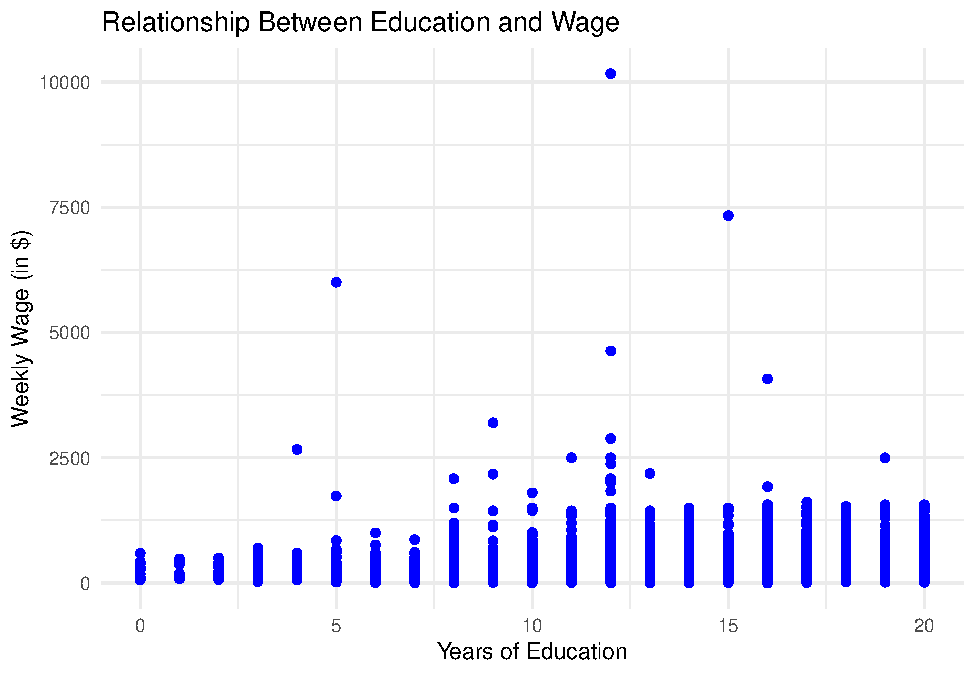
\includegraphics{Data-exploration_files/figure-latex/plot-1.pdf}

\section{\texorpdfstring{\textbf{3.Estimate the baseline
Specification}}{3.Estimate the baseline Specification}}\label{estimate-the-baseline-specification}

\begin{Shaded}
\begin{Highlighting}[]
\CommentTok{\#linear model}
\NormalTok{linear\_model1}\OtherTok{=}\FunctionTok{lm}\NormalTok{(WAGE}\SpecialCharTok{\textasciitilde{}}\NormalTok{ EDUC }\SpecialCharTok{+}\NormalTok{ AGE }\SpecialCharTok{+}\NormalTok{ RACE }\SpecialCharTok{+}\NormalTok{ SMSA }\SpecialCharTok{+}\NormalTok{ MARRIED }\SpecialCharTok{+}\NormalTok{ REGION2 }\SpecialCharTok{+}\NormalTok{ REGION3 }
                 \SpecialCharTok{+}\NormalTok{ REGION4 }\SpecialCharTok{+}\NormalTok{ REGION5 }\SpecialCharTok{+}\NormalTok{ REGION6 }\SpecialCharTok{+}\NormalTok{ REGION7 }\SpecialCharTok{+}\NormalTok{ REGION8 }\SpecialCharTok{+}\NormalTok{ REGION9  , }\AttributeTok{data =}\NormalTok{ df)}
\end{Highlighting}
\end{Shaded}

\begin{verbatim}
## 
## ==========================================================
##                              Dependent variable:          
##                     --------------------------------------
##                                      WAGE                 
## ----------------------------------------------------------
## EDUC                              26.696***               
##                                    (0.869)                
##                                   t = 30.724              
##                                   p = 0.000               
## AGE                                2.244**                
##                                    (0.942)                
##                                   t = 2.382               
##                                   p = 0.018               
## RACE                              -77.632***              
##                                    (10.225)               
##                                   t = -7.592              
##                                   p = 0.000               
## SMSA                              -63.756***              
##                                    (7.393)                
##                                   t = -8.624              
##                                   p = 0.000               
## MARRIED                           78.001***               
##                                    (8.026)                
##                                   t = 9.719               
##                                   p = 0.000               
## REGION2                           41.193***               
##                                    (13.644)               
##                                   t = 3.019               
##                                   p = 0.003               
## REGION3                           49.088***               
##                                    (13.305)               
##                                   t = 3.690               
##                                   p = 0.0003              
## REGION4                             18.845                
##                                    (15.600)               
##                                   t = 1.208               
##                                   p = 0.228               
## REGION5                             4.205                 
##                                    (13.492)               
##                                   t = 0.312               
##                                   p = 0.756               
## REGION6                             7.604                 
##                                    (16.123)               
##                                   t = 0.472               
##                                   p = 0.638               
## REGION7                             17.081                
##                                    (14.646)               
##                                   t = 1.166               
##                                   p = 0.244               
## REGION8                             15.897                
##                                    (17.106)               
##                                   t = 0.929               
##                                   p = 0.353               
## REGION9                           63.710***               
##                                    (14.046)               
##                                   t = 4.536               
##                                  p = 0.00001              
## Constant                           -81.669*               
##                                    (46.614)               
##                                   t = -1.752              
##                                   p = 0.080               
## ----------------------------------------------------------
## Observations                        10,000                
## R2                                  0.134                 
## Adjusted R2                         0.133                 
## Residual Std. Error          275.029 (df = 9986)          
## F Statistic         118.953*** (df = 13; 9986) (p = 0.000)
## ==========================================================
## Note:                          *p<0.1; **p<0.05; ***p<0.01
\end{verbatim}

\subsubsection{\texorpdfstring{\textbf{3.1 Interpretation of the
estimated Coefficient
}}{3.1 Interpretation of the estimated Coefficient }}\label{interpretation-of-the-estimated-coefficient}

EDUC (26.696, p \textless{} 0.001)

A one-year increase in education leads to a \$26.696 increase in weelky
wages. This is highly significant (p = 0.000).

AGE ( 2.244, p = 0.020) A one-year increase in age increases wages by
\$2.23. Significant at the 5\% level (p = 0.020).

RACE (-77.478, p \textless{} 0.001) Suggests a wage penalty of \$77.48
for certain racial groups (assuming a binary variable where non-white =
1). Highly significant (p = 0.000).

SMSA (-63.654, p \textless{} 0.001) Living in an SMSA (Standard
Metropolitan Statistical Area) is associated with a \$63.65 lower wage.
Significant at p = 0.000.

MARRIED (77.927, p \textless{} 0.001) Being married increases wages by
\$77.93. Highly significant (p = 0.000).

Regional Effects on Wages

Significant Regions: REGION2 (B = 41.204, p = 0.003) REGION3 (B =
49.071, p = 0.0003) REGION9 (B = 63.543, p = 0.00001) These regions have
higher wages compared to the reference region.

Non-Significant Regions: REGION4, REGION5, REGION6, REGION7, REGION8 (p
\textgreater{} 0.05) These regions do not significantly differ from the
reference region in terms of wages.

\begin{verbatim}
## 
## Linear hypothesis test:
## AGE = 0
## RACE = 0
## MARRIED = 0
## SMSA = 0
## 
## Model 1: restricted model
## Model 2: WAGE ~ EDUC + AGE + RACE + SMSA + MARRIED + REGION2 + REGION3 + 
##     REGION4 + REGION5 + REGION6 + REGION7 + REGION8 + REGION9
## 
##   Res.Df       RSS Df Sum of Sq      F    Pr(>F)    
## 1   9990 773577022                                  
## 2   9986 755352847  4  18224175 60.232 < 2.2e-16 ***
## ---
## Signif. codes:  0 '***' 0.001 '**' 0.01 '*' 0.05 '.' 0.1 ' ' 1
\end{verbatim}

The joint significance test shows that AGE, RACE, MARRIED, and SMSA
jointly contribute significantly to explaining WAGE. The F-statistic is
60.23 with a p-value \textless{} 2.2e-16, indicating strong statistical
significance. We reject the null hypothesis that these four variables
have no joint effect on wages.

\begin{verbatim}
## 
## Linear hypothesis test:
## REGION2 = 0
## REGION3 = 0
## REGION4 = 0
## REGION5 = 0
## REGION6 = 0
## REGION7 = 0
## REGION8 = 0
## REGION9 = 0
## 
## Model 1: restricted model
## Model 2: WAGE ~ EDUC + AGE + RACE + SMSA + MARRIED + REGION2 + REGION3 + 
##     REGION4 + REGION5 + REGION6 + REGION7 + REGION8 + REGION9
## 
##   Res.Df       RSS Df Sum of Sq      F    Pr(>F)    
## 1   9994 759957235                                  
## 2   9986 755352847  8   4604388 7.6089 3.389e-10 ***
## ---
## Signif. codes:  0 '***' 0.001 '**' 0.01 '*' 0.05 '.' 0.1 ' ' 1
\end{verbatim}

Since the p-value is extremely small (\textless0.001), we reject the
null hypothesis. This means that at least one of the region coefficients
is significantly different from zero, implying that region does have a
statistically significant effect on wages.

\section{\texorpdfstring{\textbf{4. Evaluating Gauss-Markov Assumptions
and Applying Remedial
Measures}}{4. Evaluating Gauss-Markov Assumptions and Applying Remedial Measures}}\label{evaluating-gauss-markov-assumptions-and-applying-remedial-measures}

\paragraph{\texorpdfstring{\textbf{4a. Stochastic
Regressors}}{4a. Stochastic Regressors}}\label{a.-stochastic-regressors}

All the variables are stochastic.

Strictly exogenous: AGE, RACE, QOB - These variables are fixed and not
influenced by wages or the error term.

Weakly exogenous: SMSA, REGION - These variables may be correlated with
unobserved factors affecting wages, but are not directly influenced by
wages.

Endogenous: EDUC, MARRIED - Potential for reverse causality or
correlation with the error term (e.g., higher wages → more education or
higher likelihood of marriage).

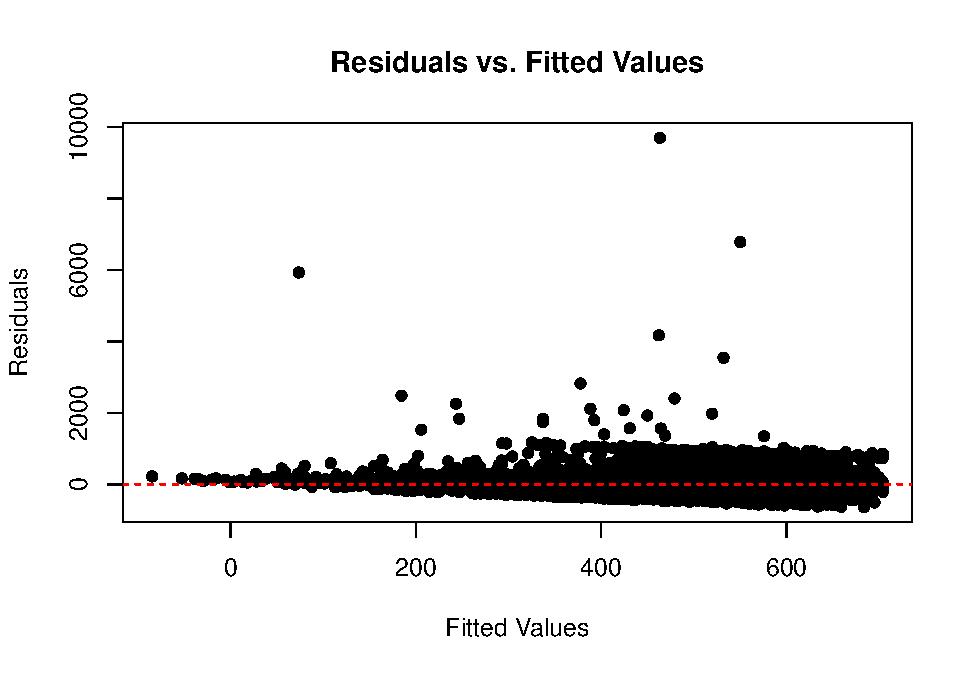
\includegraphics{Data-exploration_files/figure-latex/residuals plot-1.pdf}

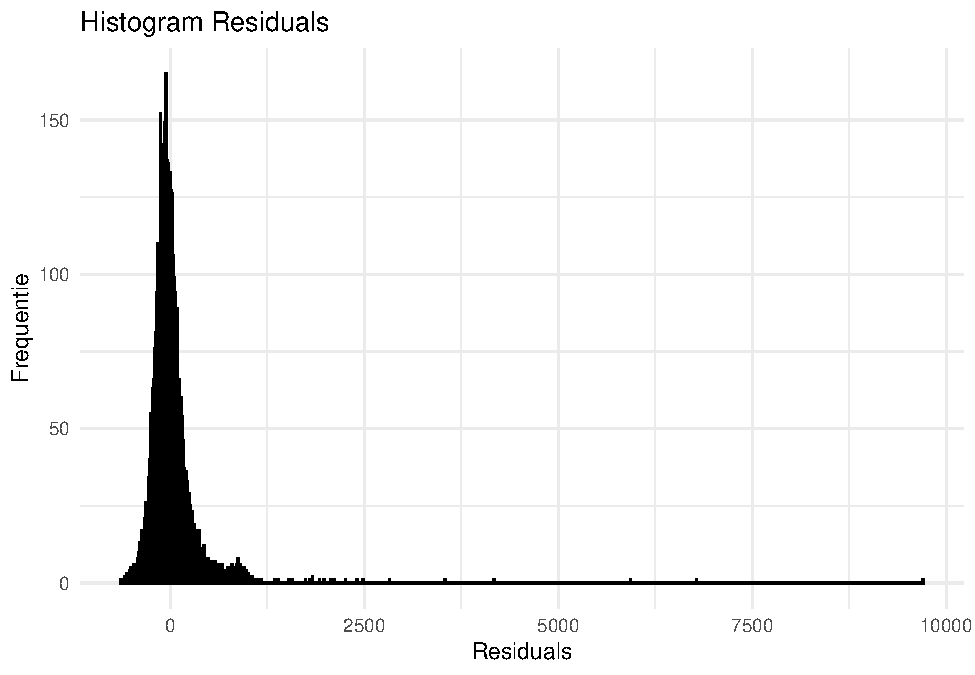
\includegraphics{Data-exploration_files/figure-latex/histogram plot-1.pdf}

\paragraph{\texorpdfstring{\textbf{4b. Normality Error
Terms}}{4b. Normality Error Terms}}\label{b.-normality-error-terms}

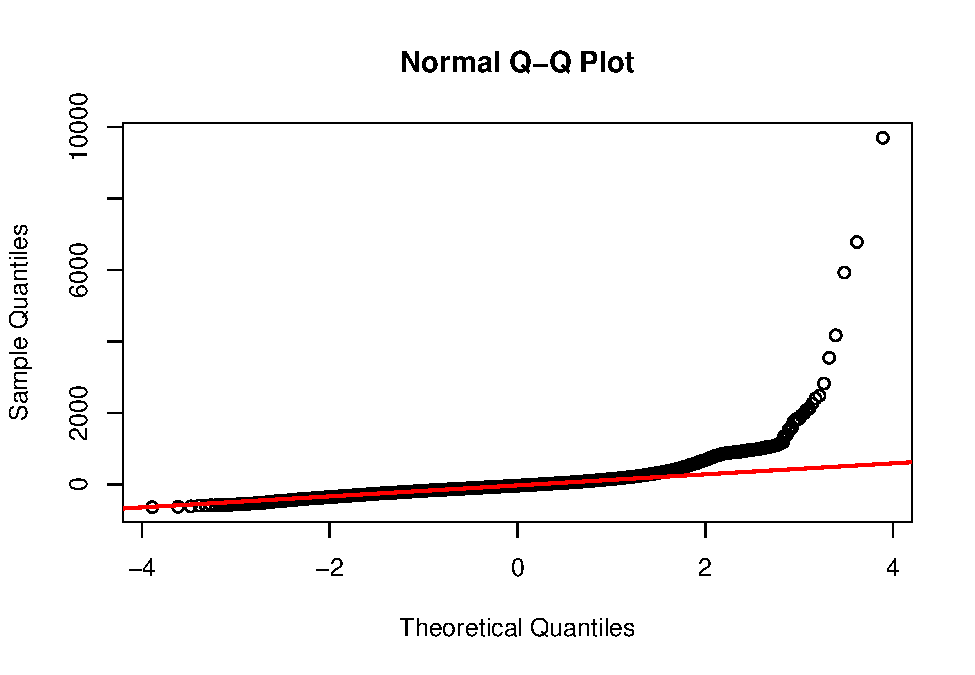
\includegraphics{Data-exploration_files/figure-latex/QQ plot-1.pdf}

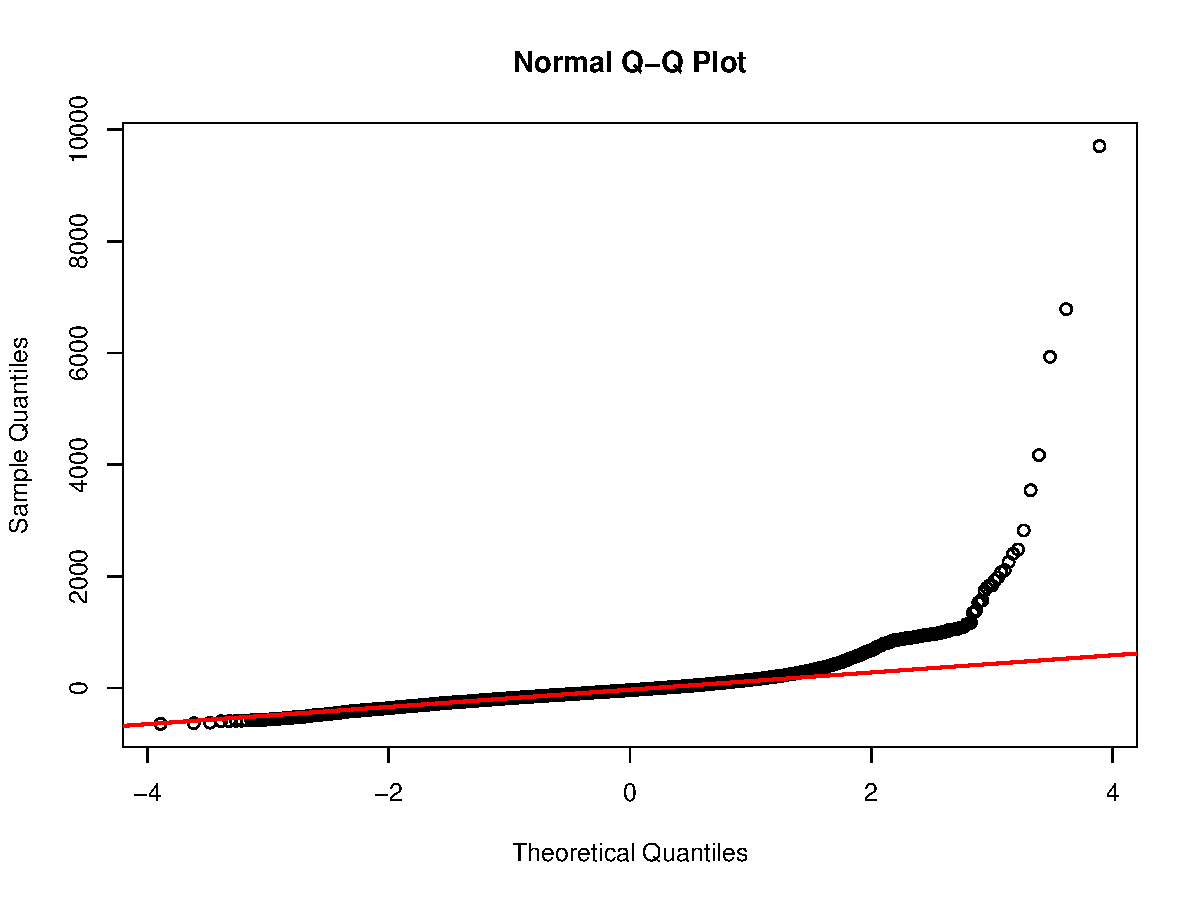
\includegraphics{Data-exploration_files/figure-latex/QQ plot_layout-1.pdf}

\begin{verbatim}
Jarque Bera Test
\end{verbatim}

data: residuals X-squared = 21722226, df = 2, p-value \textless{}
2.2e-16

Since the p value is small, we reject the null hypothesis. Therefore the
residuals are NOT normally distributed.

Implications for OLS:

\begin{enumerate}
\def\labelenumi{\arabic{enumi})}
\item
  Unbiasedness: Non-normal residuals do not affect the unbiasedness of
  OLS estimators as long as key assumptions (like linearity, exogeneity
  of regressors, and zero-mean error term) are satisfied.
\item
  Efficiency: OLS estimators may lose their efficiency because normality
  of residuals is necessary for OLS to be the Best Linear Unbiased
  Estimator (BLUE) under the Gauss-Markov assumptions.
\item
  Hypothesis Testing: The validity of tests (e.g., t-tests and F-tests)
  and confidence intervals relies on the normality assumption.
  Non-normal residuals can lead to incorrect p-values.
\item
  Heteroscedasticity or Outliers: Non-normality can signal issues like
  heteroscedasticity (non-constant error variance), the presence of
  outliers, or omitted variable bias.
\end{enumerate}

Remediation: Based on the histogram and Q-Q Plot which is slightly
right-skewed, we can conclude that the residuals deviate slightly from
normality, so OLS may still perform adequately, particularly in our
large sample where asymptotic normality applies.

\#\#\#\textbf{Gauss-Markov assumptions}:

Assumption 1: Linearity in the parameters: CHECK

Assumption 2a: The X -values are fixed over repeated sampling (fixed
regressor model) FAIL

Correlation between explanatory variables and error terms:

\begin{Shaded}
\begin{Highlighting}[]
\FunctionTok{print}\NormalTok{(}\FunctionTok{mean}\NormalTok{(residuals))}
\end{Highlighting}
\end{Shaded}

\begin{verbatim}
## [1] -4.605628e-16
\end{verbatim}

\begin{Shaded}
\begin{Highlighting}[]
\FunctionTok{print}\NormalTok{(}\FunctionTok{t.test}\NormalTok{(residuals, }\AttributeTok{mu =} \DecValTok{0}\NormalTok{))}
\end{Highlighting}
\end{Shaded}

\begin{verbatim}
## 
##  One Sample t-test
## 
## data:  residuals
## t = -1.6757e-16, df = 9999, p-value = 1
## alternative hypothesis: true mean is not equal to 0
## 95 percent confidence interval:
##  -5.387624  5.387624
## sample estimates:
##     mean of x 
## -4.605628e-16
\end{verbatim}

\begin{Shaded}
\begin{Highlighting}[]
\ControlFlowTok{if}\NormalTok{ (show\_interpretation) \{}
  \FunctionTok{cat}\NormalTok{(}\StringTok{"Assumption 3: The expected V value of the error terms is zero: CHECK"}\NormalTok{)}
\NormalTok{\}}
\end{Highlighting}
\end{Shaded}

\begin{verbatim}
## Assumption 3: The expected V value of the error terms is zero: CHECK
\end{verbatim}

\subsubsection{\texorpdfstring{\textbf{4(d)
Heteroskedasticity}}{4(d) Heteroskedasticity}}\label{d-heteroskedasticity}

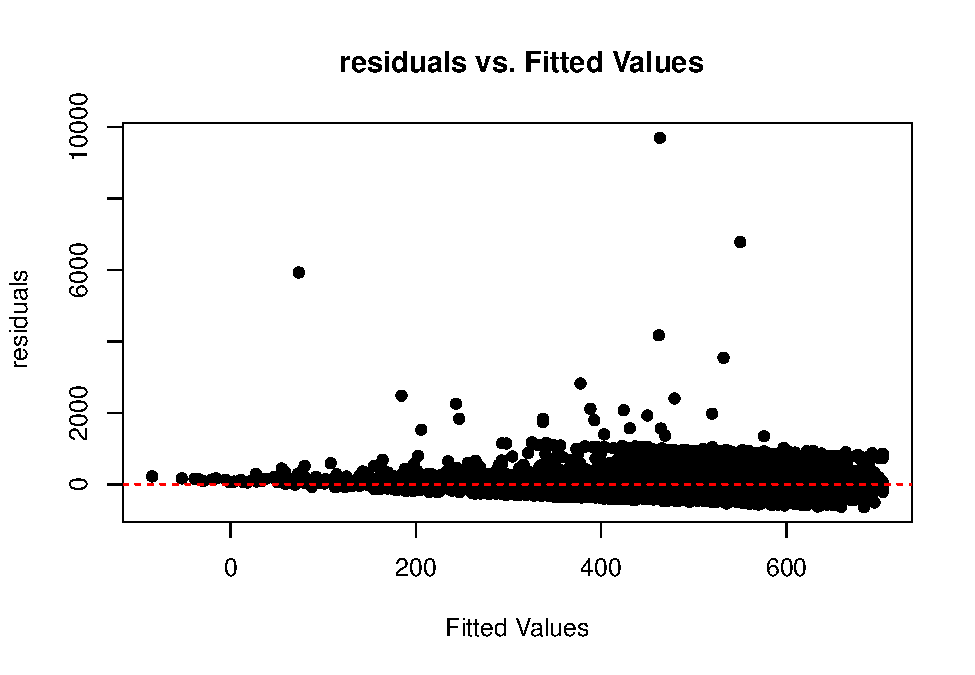
\includegraphics{Data-exploration_files/figure-latex/residuals_plot-1.pdf}
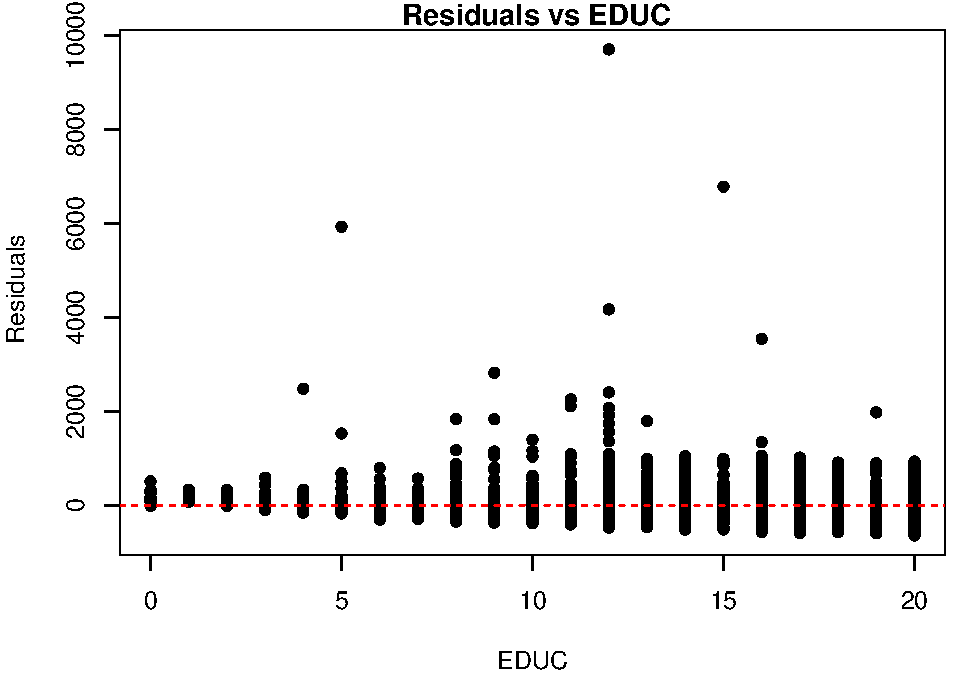
\includegraphics{Data-exploration_files/figure-latex/residuals_plot-2.pdf}
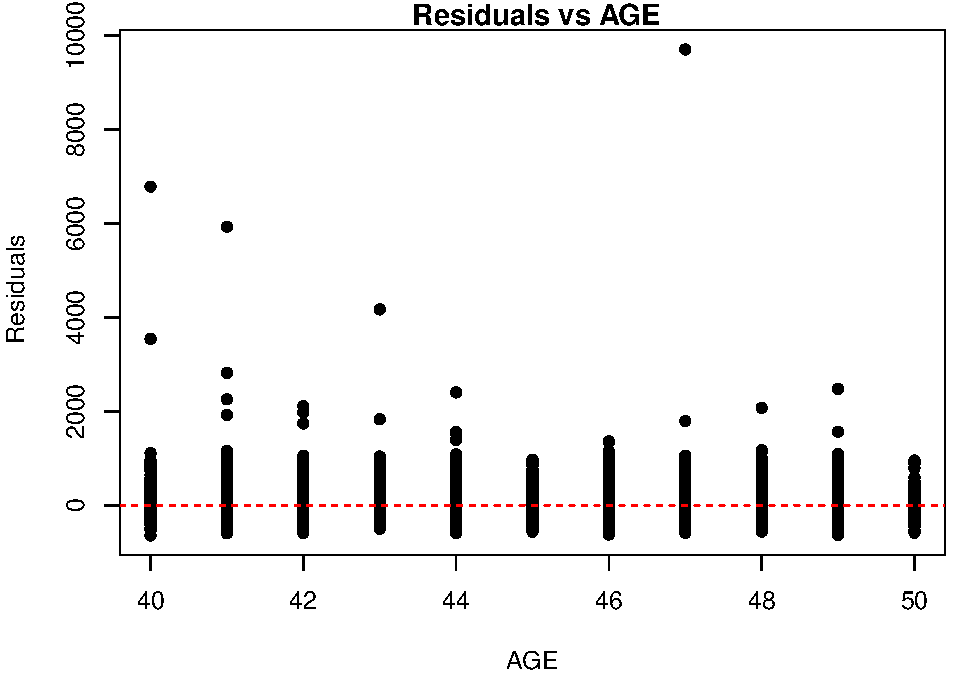
\includegraphics{Data-exploration_files/figure-latex/residuals_plot-3.pdf}
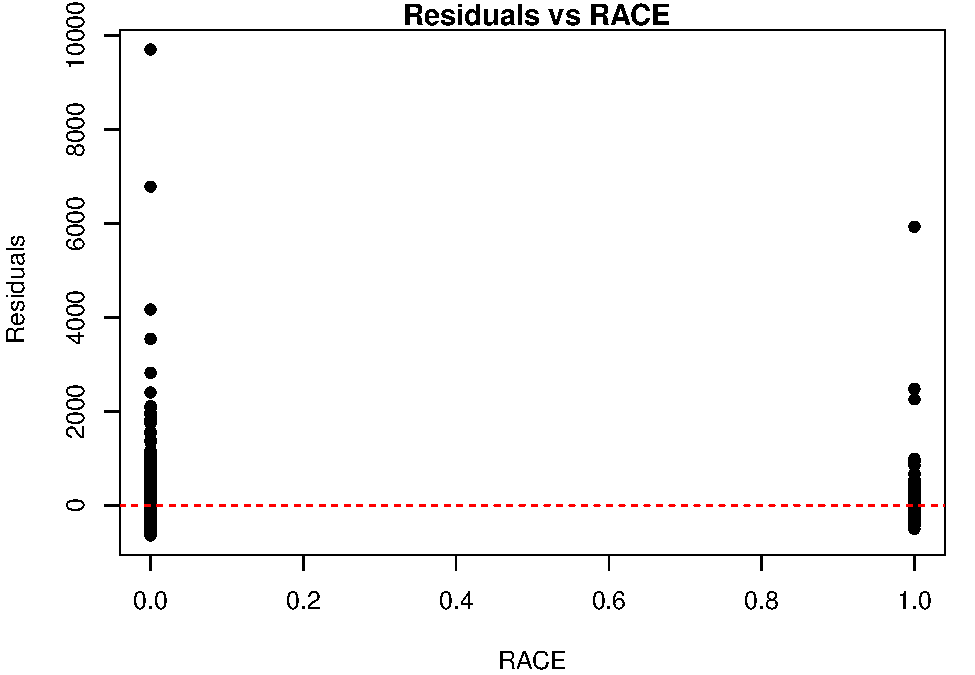
\includegraphics{Data-exploration_files/figure-latex/residuals_plot-4.pdf}
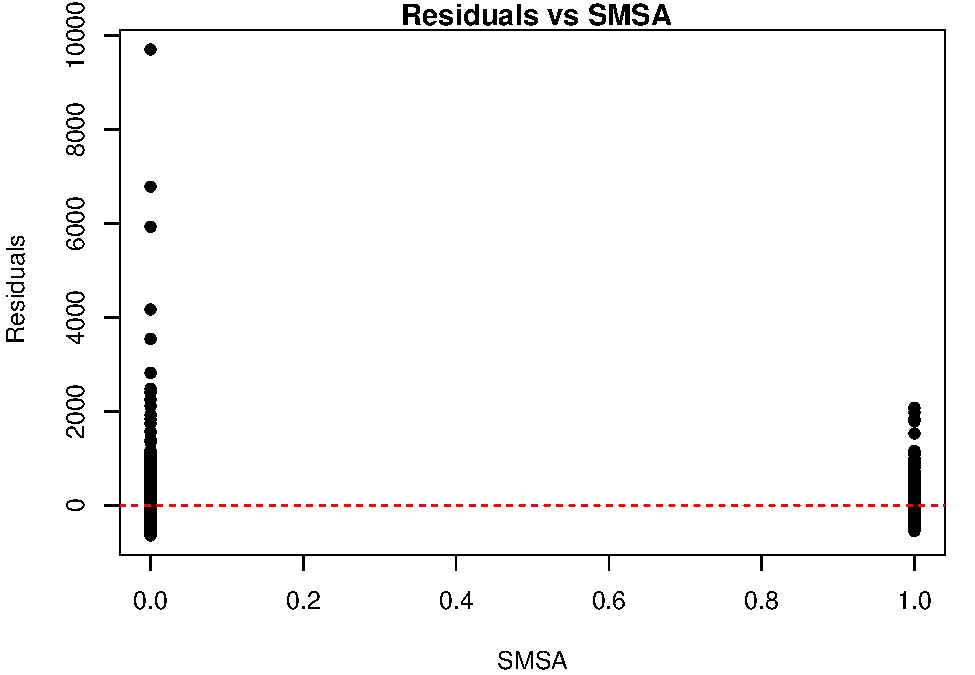
\includegraphics{Data-exploration_files/figure-latex/residuals_plot-5.pdf}
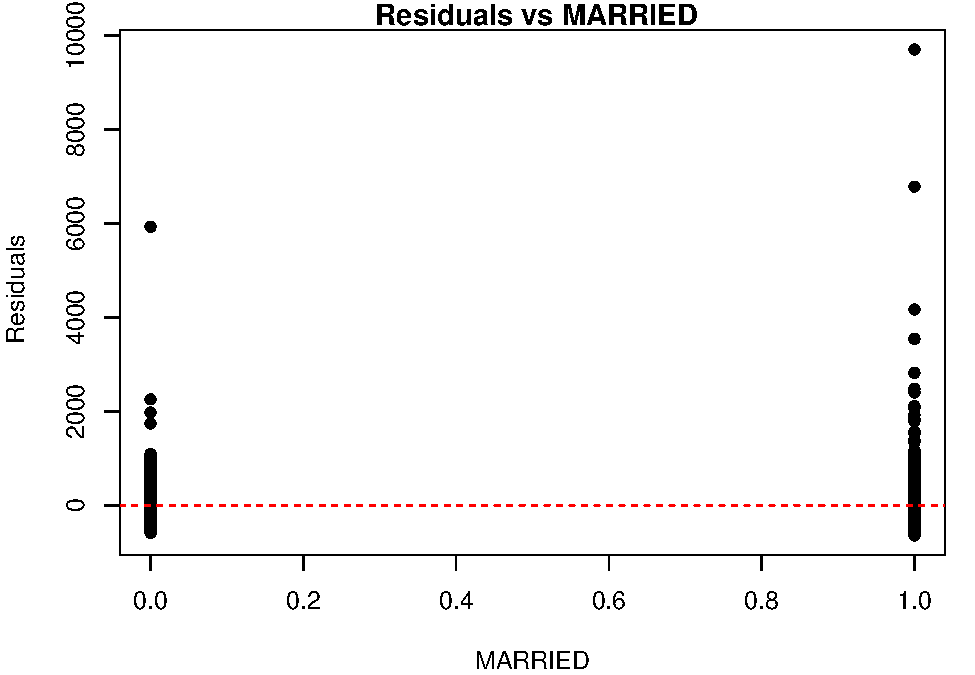
\includegraphics{Data-exploration_files/figure-latex/residuals_plot-6.pdf}
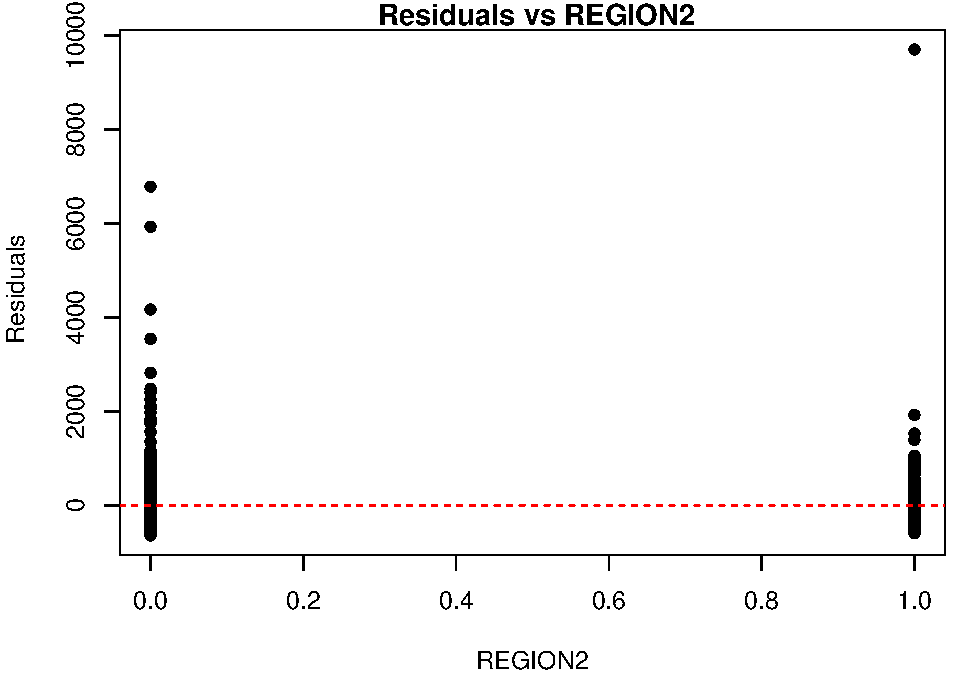
\includegraphics{Data-exploration_files/figure-latex/residuals_plot-7.pdf}
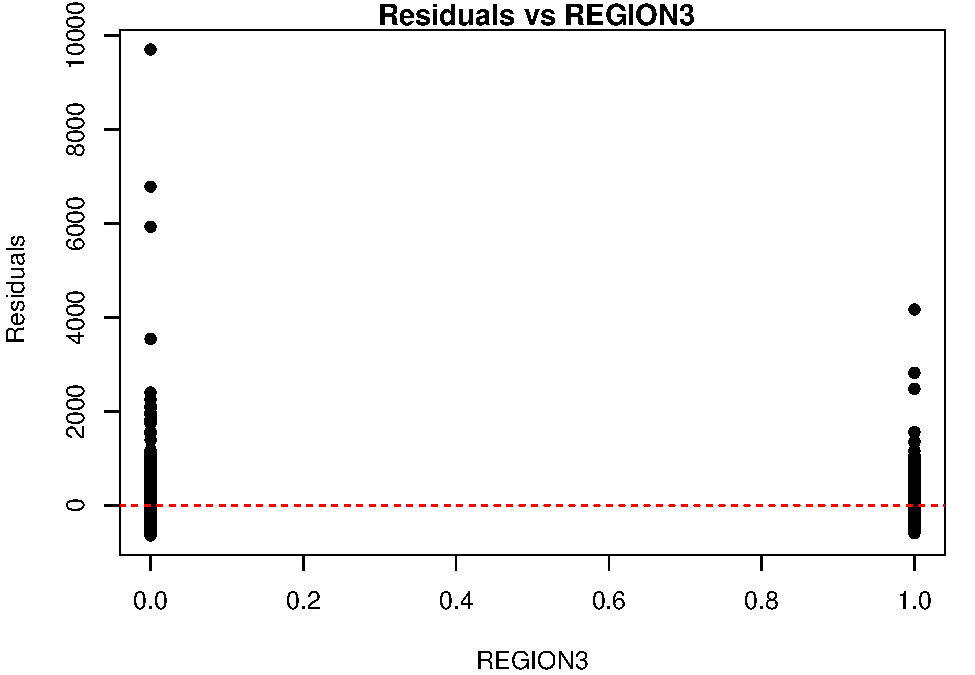
\includegraphics{Data-exploration_files/figure-latex/residuals_plot-8.pdf}
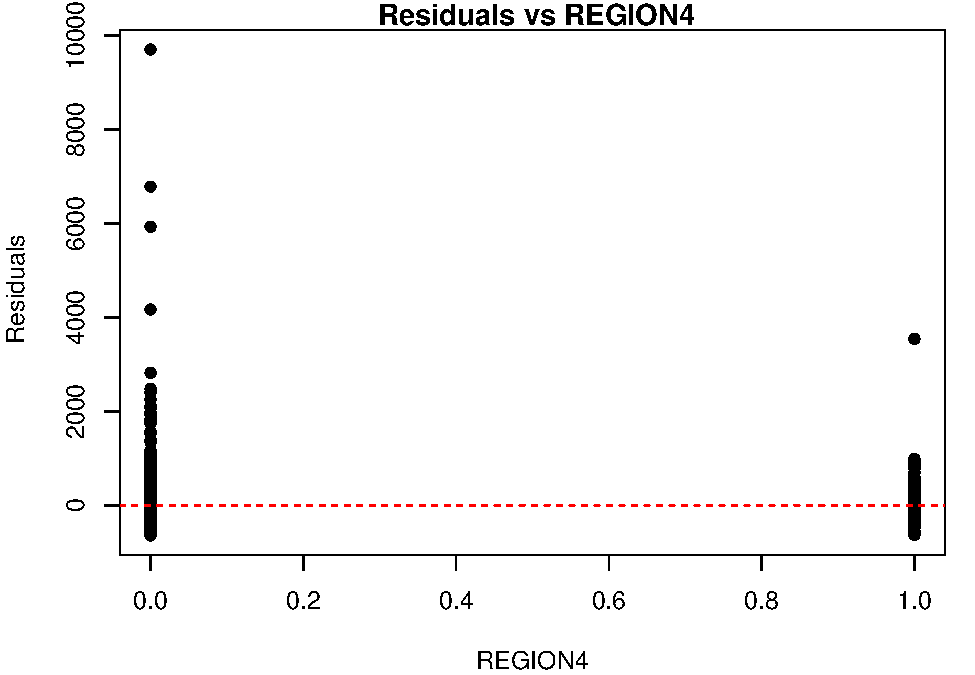
\includegraphics{Data-exploration_files/figure-latex/residuals_plot-9.pdf}
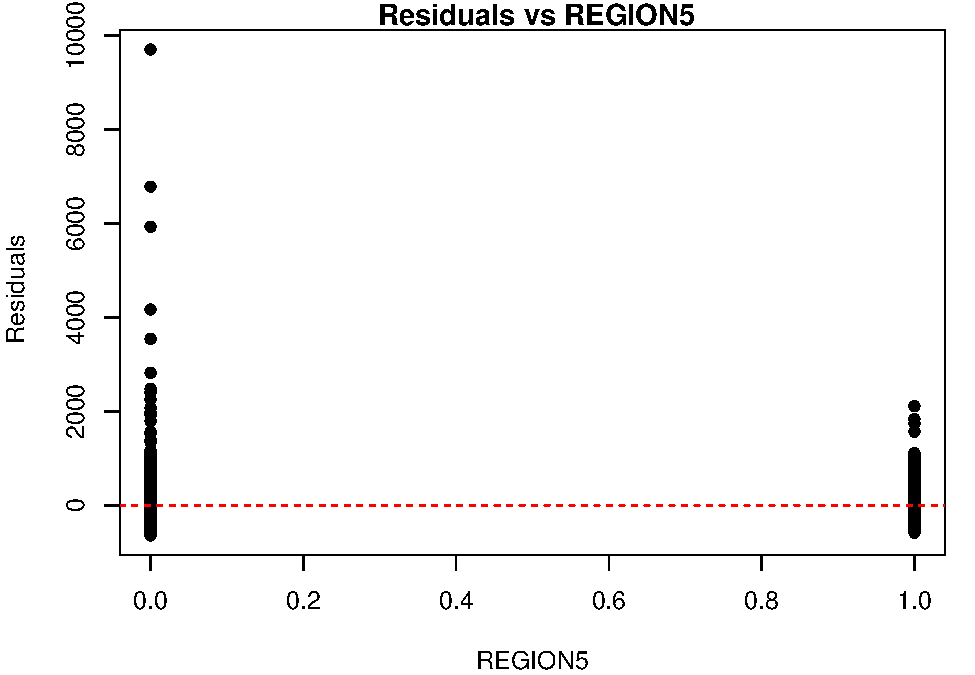
\includegraphics{Data-exploration_files/figure-latex/residuals_plot-10.pdf}
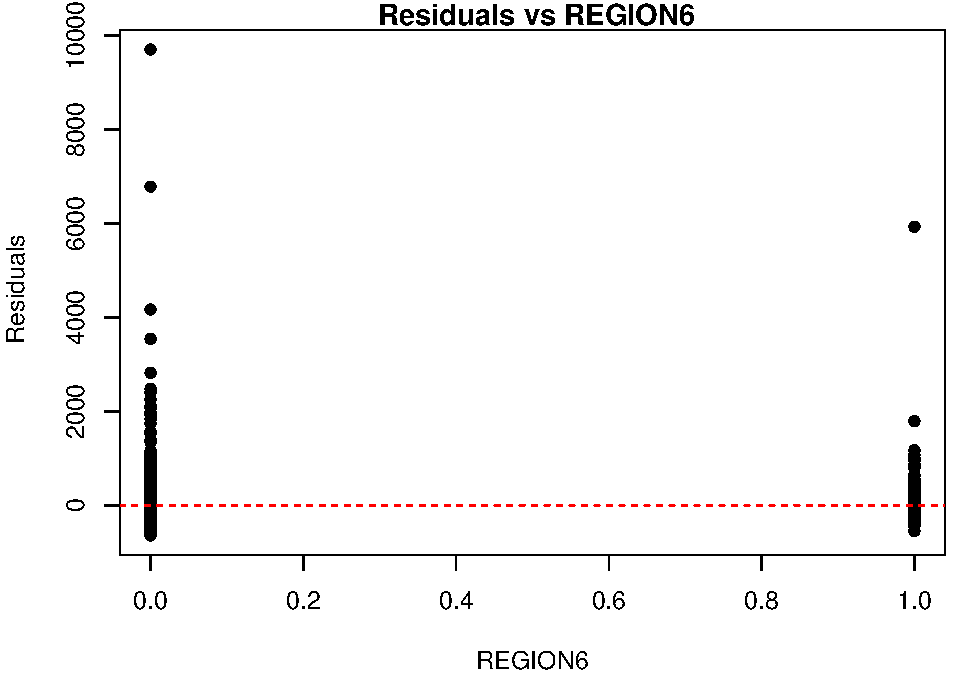
\includegraphics{Data-exploration_files/figure-latex/residuals_plot-11.pdf}
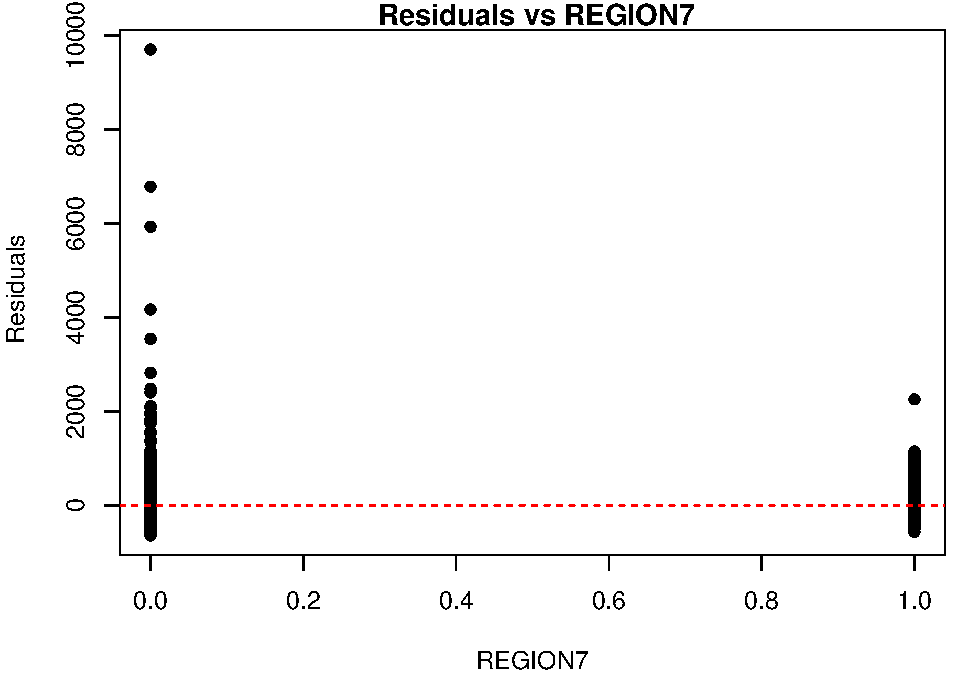
\includegraphics{Data-exploration_files/figure-latex/residuals_plot-12.pdf}
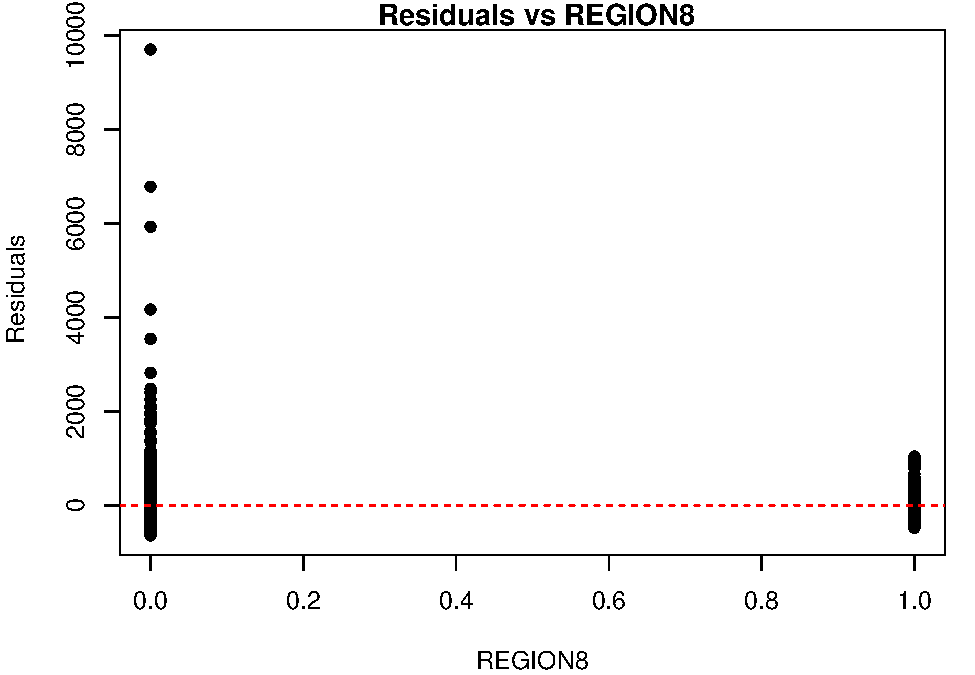
\includegraphics{Data-exploration_files/figure-latex/residuals_plot-13.pdf}
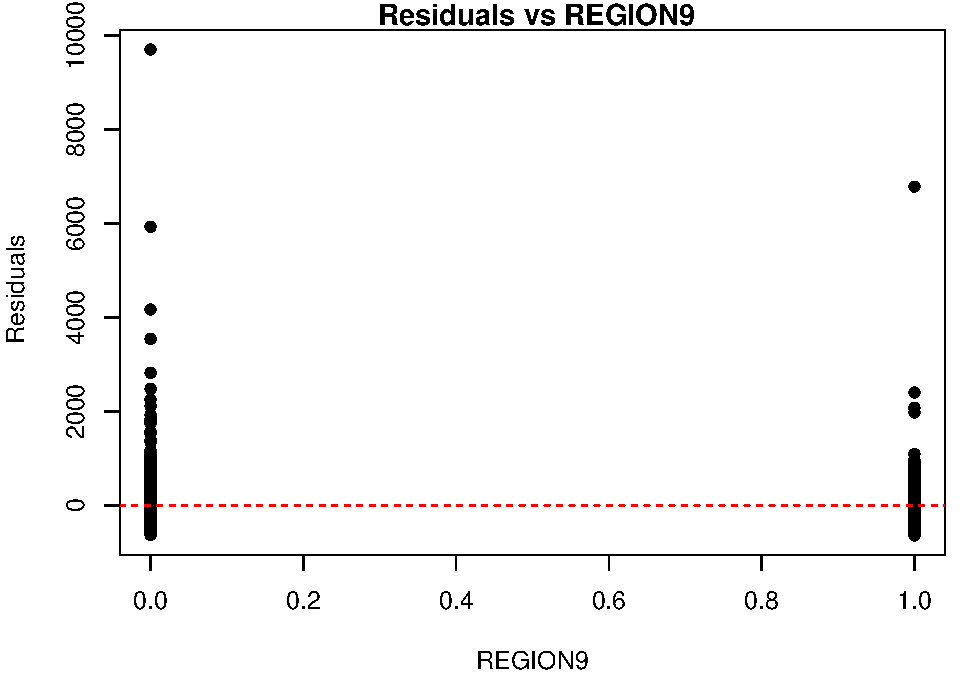
\includegraphics{Data-exploration_files/figure-latex/residuals_plot-14.pdf}

\subsubsection{Interpretation of Residual
Plots:}\label{interpretation-of-residual-plots}

\begin{enumerate}
\def\labelenumi{\arabic{enumi}.}
\tightlist
\item
  \textbf{Fitted Values}:

  \begin{itemize}
  \tightlist
  \item
    Slight increase in spread as fitted values increase
  \item
    This pattern indicates potential heteroskedasticity
  \end{itemize}
\item
  \textbf{EDUC}:

  \begin{itemize}
  \tightlist
  \item
    Initial increase followed by decrease in spread
  \item
    Non-constant variance pattern visible
  \end{itemize}
\item
  \textbf{RACE}:

  \begin{itemize}
  \tightlist
  \item
    Larger spread observed for white participants
  \item
    Unequal variance between groups
  \end{itemize}
\item
  \textbf{SMSA}:

  \begin{itemize}
  \tightlist
  \item
    Non-metropolitan areas show greater spread
  \item
    Variance differs by urban/rural classification
  \end{itemize}
\item
  \textbf{MARRIED}:

  \begin{itemize}
  \tightlist
  \item
    Similar variance pattern as other categorical variables
  \end{itemize}
\item
  \textbf{REGION}:

  \begin{itemize}
  \tightlist
  \item
    Different spreads observed across regions (0-1 range)
  \item
    Geographic heterogeneity in variance
  \end{itemize}
\end{enumerate}

\textbf{Conclusion}:

Clear signs of heteroskedasticity across multiple predictors, suggesting
violations of the constant variance assumption.

\subsection{\texorpdfstring{\textbf{4(d).1}Heteroskedasticity test
**}{4(d).1Heteroskedasticity test **}}\label{d.1heteroskedasticity-test}

\paragraph{\texorpdfstring{\textbf{white's general
test}}{white's general test}}\label{whites-general-test}

\begin{Shaded}
\begin{Highlighting}[]
\NormalTok{white\_test }\OtherTok{\textless{}{-}} \FunctionTok{bptest}\NormalTok{(linear\_model1, }\SpecialCharTok{\textasciitilde{}} \FunctionTok{fitted}\NormalTok{(linear\_model1) }\SpecialCharTok{+} \FunctionTok{I}\NormalTok{(}\FunctionTok{fitted}\NormalTok{(linear\_model1)}\SpecialCharTok{\^{}}\DecValTok{2}\NormalTok{))}
\FunctionTok{print}\NormalTok{(white\_test)}
\end{Highlighting}
\end{Shaded}

\begin{verbatim}
studentized Breusch-Pagan test
\end{verbatim}

data: linear\_model1 BP = 7.0287, df = 2, p-value = 0.02977

the p value of 0.02977 says that we reject the null hyptothis , which
implies that we reject homoskedastiscity

\textbf{properties}

-for white there are not properties

\paragraph{\texorpdfstring{\textbf{goldfeld-quant
test}}{goldfeld-quant test}}\label{goldfeld-quant-test}

\begin{Shaded}
\begin{Highlighting}[]
\NormalTok{gqtest\_result }\OtherTok{\textless{}{-}} \FunctionTok{gqtest}\NormalTok{(linear\_model1)}
\FunctionTok{print}\NormalTok{(gqtest\_result)}
\end{Highlighting}
\end{Shaded}

\begin{verbatim}
Goldfeld-Quandt test
\end{verbatim}

data: linear\_model1 GQ = 1.1763, df1 = 4986, df2 = 4986, p-value =
5.067e-09 alternative hypothesis: variance increases from segment 1 to 2

the p value of p-value = 5.067e-09 says that we strongly reject the null
hyptothis , which implies that we reject homoskedastiscity

\textbf{properties}

-You split the dataset into two non-overlapping groups (dropping middle
observations).

-Errors are normally distributed., but in our case they are not so be
carefull with the interpratation of this test \textbf{Implications for
OLS Estimators}

-the coef( the betas ) are not normally distr in small samples

-var of the coef changes , we have a more robust variance formula if we
use OLS

-OLS is no longer effecient , we use UGLS wich has a lower variance of
the estimator

-the st errors of the coef are underestimated and are not to be trusted,
therefore infernce bout the significance is wrong \#\# \textbf{4(d).2
adressing heteroskedasticity}

\% Table created by stargazer v.5.2.3 by Marek Hlavac, Social Policy
Institute. E-mail: marek.hlavac at gmail.com \% Date and time: vr, mei
02, 2025 - 13:45:27

\begin{table}[!htbp] \centering 
  \caption{OLS Regression with Robust Standard Errors} 
  \label{} 
\begin{tabular}{@{\extracolsep{5pt}}lc} 
\\[-1.8ex]\hline 
\hline \\[-1.8ex] 
 & \multicolumn{1}{c}{\textit{Dependent variable:}} \\ 
\cline{2-2} 
\\[-1.8ex] & Weekly Wage \\ 
\hline \\[-1.8ex] 
 Education & 26.6959$^{***}$ \\ 
  & (0.9195) \\ 
  & \\ 
 Age & 2.2442$^{**}$ \\ 
  & (0.9904) \\ 
  & \\ 
 Race (1=Black) & $-$77.6318$^{***}$ \\ 
  & (9.3993) \\ 
  & \\ 
 SMSA & $-$63.7562$^{***}$ \\ 
  & (6.2933) \\ 
  & \\ 
 Married & 78.0013$^{***}$ \\ 
  & (7.9377) \\ 
  & \\ 
 Region 2 & 41.1931$^{***}$ \\ 
  & (12.5820) \\ 
  & \\ 
 Region 3 & 49.0879$^{***}$ \\ 
  & (10.7642) \\ 
  & \\ 
 Region 4 & 18.8453 \\ 
  & (12.9618) \\ 
  & \\ 
 Region 5 & 4.2049 \\ 
  & (10.9000) \\ 
  & \\ 
 Region 6 & 7.6044 \\ 
  & (15.3990) \\ 
  & \\ 
 Region 7 & 17.0805 \\ 
  & (12.0089) \\ 
  & \\ 
 Region 8 & 15.8968 \\ 
  & (13.7353) \\ 
  & \\ 
 Region 9 & 63.7105$^{***}$ \\ 
  & (13.0419) \\ 
  & \\ 
 Constant & $-$81.6693 \\ 
  & (49.8668) \\ 
  & \\ 
\hline \\[-1.8ex] 
Observations & 10,000 \\ 
R$^{2}$ & 0.1341 \\ 
Adjusted R$^{2}$ & 0.1330 \\ 
Residual Std. Error & 275.0294 (df = 9986) \\ 
F Statistic & 118.9531$^{***}$ (df = 13; 9986) \\ 
\hline 
\hline \\[-1.8ex] 
\textit{Note:}  & \multicolumn{1}{r}{$^{*}$p$<$0.1; $^{**}$p$<$0.05; $^{***}$p$<$0.01} \\ 
 & \multicolumn{1}{r}{Heteroskedasticity-consistent standard errors in parentheses} \\ 
\end{tabular} 
\end{table}

\subparagraph{**Interpretation:}\label{interpretation}

**- Robust standard errors are larger than conventional OLS standard
errors - This pattern confirms the presence of heteroskedasticity in the
data - The HC1 estimator provides consistent inference under
heteroskedasticity - Coefficient estimates remain unchanged, but
significance levels may differ

\textbf{EGLS}

\begin{Shaded}
\begin{Highlighting}[]
\NormalTok{gls\_model }\OtherTok{\textless{}{-}} \FunctionTok{gls}\NormalTok{(WAGE}\SpecialCharTok{\textasciitilde{}}\NormalTok{ EDUC }\SpecialCharTok{+}\NormalTok{ AGE }\SpecialCharTok{+}\NormalTok{ RACE }\SpecialCharTok{+}\NormalTok{ SMSA }\SpecialCharTok{+}\NormalTok{ MARRIED }\SpecialCharTok{+}\NormalTok{ REGION2 }\SpecialCharTok{+}\NormalTok{ REGION3 }
                 \SpecialCharTok{+}\NormalTok{ REGION4 }\SpecialCharTok{+}\NormalTok{ REGION5 }\SpecialCharTok{+}\NormalTok{ REGION6 }\SpecialCharTok{+}\NormalTok{ REGION7 }\SpecialCharTok{+}\NormalTok{ REGION8 }\SpecialCharTok{+}\NormalTok{ REGION9  , }\AttributeTok{data =}\NormalTok{ df)}
\NormalTok{                 weights }\OtherTok{=} \FunctionTok{varIdent}\NormalTok{(}\AttributeTok{form =} \SpecialCharTok{\textasciitilde{}}\DecValTok{1} \SpecialCharTok{|}\NormalTok{ EDC)}
\end{Highlighting}
\end{Shaded}

\% Table created by stargazer v.5.2.3 by Marek Hlavac, Social Policy
Institute. E-mail: marek.hlavac at gmail.com \% Date and time: vr, mei
02, 2025 - 13:45:27

\begin{table}[!htbp] \centering 
  \caption{EGLS Estimation Results} 
  \label{} 
\begin{tabular}{@{\extracolsep{1pt}}lc} 
\\[-1.8ex]\hline 
\hline \\[-1.8ex] 
 & \multicolumn{1}{c}{\textit{Dependent variable:}} \\ 
\cline{2-2} 
\\[-1.8ex] & Weekly Wages \\ 
\hline \\[-1.8ex] 
 Education & 26.696$^{***}$ (0.869) \\ 
  Age & 2.244$^{**}$ (0.942) \\ 
  Race (1=Black) & $-$77.632$^{***}$ (10.225) \\ 
  SMSA & $-$63.756$^{***}$ (7.393) \\ 
  Married & 78.001$^{***}$ (8.026) \\ 
  Region 2 & 41.193$^{***}$ (13.644) \\ 
  Region 3 & 49.088$^{***}$ (13.305) \\ 
  Region 4 & 18.845 (15.600) \\ 
  Region 5 & 4.205 (13.492) \\ 
  Region 6 & 7.604 (16.123) \\ 
  Region 7 & 17.081 (14.646) \\ 
  Region 8 & 15.897 (17.106) \\ 
  Region 9 & 63.710$^{***}$ (14.046) \\ 
  Constant & $-$81.669$^{*}$ (46.614) \\ 
 \hline \\[-1.8ex] 
Observations & 10,000 \\ 
Log Likelihood & $-$70,312.600 \\ 
Akaike Inf. Crit. & 140,655.200 \\ 
Bayesian Inf. Crit. & 140,763.300 \\ 
\hline 
\hline \\[-1.8ex] 
\textit{Note:}  & \multicolumn{1}{r}{$^{*}$p$<$0.1; $^{**}$p$<$0.05; $^{***}$p$<$0.01} \\ 
 & \multicolumn{1}{r}{Standard errors in parentheses} \\ 
\end{tabular} 
\end{table}

\subparagraph{\texorpdfstring{\textbf{Comparison with Robust Standard
Errors:}}{Comparison with Robust Standard Errors:}}\label{comparison-with-robust-standard-errors}

\begin{itemize}
\tightlist
\item
  EGLS provides more efficient estimates than OLS with robust standard
  errors
\item
  Standard errors are typically larger than OLS with incorrect variance
  formula
\item
  The efficiency gain comes from properly modeling the
  heteroskedasticity structure
\item
  Interpretation of coefficients remains the same as OLS
\end{itemize}

\begin{verbatim}

Multicollinearity

      Gauss-Markov assumption (no perfect multicollinearity) is met.
      

      Analysis of Variance Inflation Factors and correlation:
      Low VIFs (<5): Most of the variables have VIF values close to 1, including EDUC (1.07), AGE (1.01), RACE (1.05), SMSA (1.07), and MARRIED (1.02). These values suggest minimal multicollinearity, meaning these predictors are relatively independent.

      
      Moderate VIFs (Between 2 and 5): Some regional variables—REGION2 (3.28), REGION3 (3.67), REGION4 (2.18), REGION5 (3.51), REGION6 (2.06), REGION7 (2.54), REGION8 (1.82), and REGION9 (2.92)—show moderate correlation with other predictors. These values indicate some degree of collinearity, but they are not alarmingly high.
      

      High VIFs (>5): None of the variables exceed 5, which suggests that severe multicollinearity is not a major issue in this regression model. But even if VIF would be high (VIF>5), a large sample (n = 10 000 in this case) and high variance
in the explanatory variables can still lead to precise estimates.

      Implications for the properties and precision of the OLS estimator:
      1) Parameters remain identifiable.

      2) Under the CNLRM assumptions, the OLS estimator remains BLUE and normally distributed.

      3) OLS estimators exhibit larger variance and covariance, especially the regions.

      4) Wider confidence intervals and lower t-statistics 
      ->variables appear less significantly different from zero, higher probability of making a Type II error

      5) The overall model fit (R2) is largely unaffected: even if individual coefficients are insignificant, the F -test may
indicate that the coefficients are jointly significant, and can be estimated with high precision.

      6) Regression coefficients may change substantially

      ![](Data-exploration_files/figure-latex/Breusch pagan interpretie-1.pdf)<!-- --> 


``` r
print(correlation_matrix)
\end{verbatim}

\begin{verbatim}
##                 EDUC          AGE         RACE        SMSA      MARRIED
## EDUC     1.000000000 -0.069506286 -0.151952924 -0.14907033  0.019198364
## AGE     -0.069506286  1.000000000 -0.005148653 -0.02085355  0.020809977
## RACE    -0.151952924 -0.005148653  1.000000000 -0.03556389 -0.113282921
## SMSA    -0.149070326 -0.020853549 -0.035563888  1.00000000  0.040644736
## MARRIED  0.019198364  0.020809977 -0.113282921  0.04064474  1.000000000
## REGION2  0.035717362  0.008497716  0.014092931 -0.10391873 -0.003692641
## REGION3 -0.030839760  0.005358420 -0.023908637 -0.02447606  0.013937881
## REGION4 -0.000578807 -0.014907585 -0.049908666  0.11787788  0.020881363
## REGION5 -0.042953090 -0.012179069  0.091472810  0.01940650  0.004255528
## REGION6 -0.084427585  0.008312525  0.039575771  0.11343959  0.017738535
## REGION7 -0.032806167  0.003156501  0.008728591 -0.01074680  0.007148294
## REGION8  0.028455078 -0.026179022 -0.043610641  0.07119329  0.020956712
## REGION9  0.104683025  0.001483814 -0.030119960 -0.07742498 -0.060808526
##              REGION2     REGION3      REGION4      REGION5      REGION6
## EDUC     0.035717362 -0.03083976 -0.000578807 -0.042953090 -0.084427585
## AGE      0.008497716  0.00535842 -0.014907585 -0.012179069  0.008312525
## RACE     0.014092931 -0.02390864 -0.049908666  0.091472810  0.039575771
## SMSA    -0.103918730 -0.02447606  0.117877877  0.019406502  0.113439595
## MARRIED -0.003692641  0.01393788  0.020881363  0.004255528  0.017738535
## REGION2  1.000000000 -0.21345470 -0.121923453 -0.201399480 -0.113442761
## REGION3 -0.213454705  1.00000000 -0.138274958 -0.228409743 -0.128656896
## REGION4 -0.121923453 -0.13827496  1.000000000 -0.130465639 -0.073487689
## REGION5 -0.201399480 -0.22840974 -0.130465639  1.000000000 -0.121390774
## REGION6 -0.113442761 -0.12865690 -0.073487689 -0.121390774  1.000000000
## REGION7 -0.144209678 -0.16355005 -0.093418354 -0.154313279 -0.086920406
## REGION8 -0.098898407 -0.11216196 -0.064065924 -0.105827415 -0.059609658
## REGION9 -0.166513184 -0.18884475 -0.107866461 -0.178179412 -0.100363538
##              REGION7     REGION8      REGION9
## EDUC    -0.032806167  0.02845508  0.104683025
## AGE      0.003156501 -0.02617902  0.001483814
## RACE     0.008728591 -0.04361064 -0.030119960
## SMSA    -0.010746803  0.07119329 -0.077424983
## MARRIED  0.007148294  0.02095671 -0.060808526
## REGION2 -0.144209678 -0.09889841 -0.166513184
## REGION3 -0.163550053 -0.11216196 -0.188844746
## REGION4 -0.093418354 -0.06406592 -0.107866461
## REGION5 -0.154313279 -0.10582742 -0.178179412
## REGION6 -0.086920406 -0.05960966 -0.100363538
## REGION7  1.000000000 -0.07577645 -0.127583227
## REGION8 -0.075776449  1.00000000 -0.087496055
## REGION9 -0.127583227 -0.08749605  1.000000000
\end{verbatim}

\begin{Shaded}
\begin{Highlighting}[]
\FunctionTok{print}\NormalTok{(}\FunctionTok{max}\NormalTok{(}\FunctionTok{abs}\NormalTok{(correlation\_matrix)))}
\end{Highlighting}
\end{Shaded}

\begin{verbatim}
## [1] 1
\end{verbatim}

\begin{Shaded}
\begin{Highlighting}[]
\FunctionTok{print}\NormalTok{(}\StringTok{\textquotesingle{}VIF values\textquotesingle{}}\NormalTok{)}
\end{Highlighting}
\end{Shaded}

\begin{verbatim}
## [1] "VIF values"
\end{verbatim}

\begin{Shaded}
\begin{Highlighting}[]
\NormalTok{vif\_values }\OtherTok{=} \FunctionTok{vif}\NormalTok{(linear\_model1)}
\FunctionTok{print}\NormalTok{(vif\_values)}
\end{Highlighting}
\end{Shaded}

\begin{verbatim}
##     EDUC      AGE     RACE     SMSA  MARRIED  REGION2  REGION3  REGION4 
## 1.072047 1.008200 1.054291 1.072522 1.019728 3.280936 3.672041 2.182705 
##  REGION5  REGION6  REGION7  REGION8  REGION9 
## 3.510183 2.058605 2.540830 1.816650 2.919060
\end{verbatim}

\begin{Shaded}
\begin{Highlighting}[]
\NormalTok{df}\SpecialCharTok{$}\NormalTok{residuals }\OtherTok{\textless{}{-}}\NormalTok{ residuals}
\NormalTok{df\_ordered }\OtherTok{\textless{}{-}}\NormalTok{ df[}\FunctionTok{order}\NormalTok{(df}\SpecialCharTok{$}\NormalTok{EDUC, df}\SpecialCharTok{$}\NormalTok{AGE), ]}
\FunctionTok{plot}\NormalTok{(df\_ordered}\SpecialCharTok{$}\NormalTok{residuals, }\AttributeTok{type =} \StringTok{"l"}\NormalTok{,}
     \AttributeTok{main =} \StringTok{"Residuals Ordered by EDUC and AGE"}\NormalTok{,}
     \AttributeTok{ylab =} \StringTok{"Residuals"}\NormalTok{, }\AttributeTok{xlab =} \StringTok{"Observation Index"}\NormalTok{)}
\end{Highlighting}
\end{Shaded}

\includegraphics{Data-exploration_files/figure-latex/autocorrelation graph-1.pdf}

\begin{Shaded}
\begin{Highlighting}[]
\FunctionTok{runs.test}\NormalTok{(df}\SpecialCharTok{$}\NormalTok{residuals)}
\end{Highlighting}
\end{Shaded}

\begin{verbatim}
## 
##  Runs Test
## 
## data:  df$residuals
## statistic = -0.22001, runs = 4990, n1 = 5000, n2 = 5000, n = 10000,
## p-value = 0.8259
## alternative hypothesis: nonrandomness
\end{verbatim}

\begin{Shaded}
\begin{Highlighting}[]
\ControlFlowTok{if}\NormalTok{ (show\_interpretation) \{}
  \FunctionTok{cat}\NormalTok{(}\StringTok{"Assumptions:}
\StringTok{  1) no need to assume specific error structure}
\StringTok{  2) The observations should be in a meaningful order as the test evaluates the sequence}
\StringTok{  High p{-}value suggest that there is no autocorrelation."}\NormalTok{)}
\NormalTok{  \}}
\end{Highlighting}
\end{Shaded}

\begin{verbatim}
## Assumptions:
##   1) no need to assume specific error structure
##   2) The observations should be in a meaningful order as the test evaluates the sequence
##   High p-value suggest that there is no autocorrelation.
\end{verbatim}

\begin{Shaded}
\begin{Highlighting}[]
\NormalTok{DW}\OtherTok{=}\FunctionTok{dwtest}\NormalTok{(linear\_model1)}
\CommentTok{\# print to screen}
\NormalTok{DW\_summary}\OtherTok{=}\FunctionTok{c}\NormalTok{(DW}\SpecialCharTok{$}\NormalTok{statistic,DW}\SpecialCharTok{$}\NormalTok{p.value)}
\FunctionTok{names}\NormalTok{(DW\_summary)}\OtherTok{=}\FunctionTok{c}\NormalTok{(}\StringTok{"Test{-}statistic"}\NormalTok{,}\StringTok{"P{-}value"}\NormalTok{)}
\FunctionTok{stargazer}\NormalTok{(DW\_summary,}\AttributeTok{type=}\StringTok{"text"}\NormalTok{)}
\end{Highlighting}
\end{Shaded}

\begin{verbatim}
## 
## ======================
## Test-statistic P-value
## ----------------------
## 2.010           0.691 
## ----------------------
\end{verbatim}

\begin{Shaded}
\begin{Highlighting}[]
\ControlFlowTok{if}\NormalTok{ (show\_interpretation) \{}
  \FunctionTok{cat}\NormalTok{(}\StringTok{"Assumptions:}
\StringTok{  1) Error terms follow an AR(1) process}
\StringTok{  2) Error terms are normally distributed}
\StringTok{  3) The regression model does not include lagged dependent variables}
\StringTok{  High p{-}value suggest that there is no autocorrelation."}\NormalTok{)}
\NormalTok{  \}}
\end{Highlighting}
\end{Shaded}

\begin{verbatim}
## Assumptions:
##   1) Error terms follow an AR(1) process
##   2) Error terms are normally distributed
##   3) The regression model does not include lagged dependent variables
##   High p-value suggest that there is no autocorrelation.
\end{verbatim}

\begin{Shaded}
\begin{Highlighting}[]
\NormalTok{BG }\OtherTok{=} \FunctionTok{bgtest}\NormalTok{(linear\_model1, }\AttributeTok{order =} \DecValTok{6}\NormalTok{)  }\CommentTok{\# Change order as needed}
\NormalTok{BG\_summary}\OtherTok{=}\FunctionTok{c}\NormalTok{(BG}\SpecialCharTok{$}\NormalTok{statistic,BG}\SpecialCharTok{$}\NormalTok{p.value)}
\FunctionTok{names}\NormalTok{(BG\_summary)}\OtherTok{=}\FunctionTok{c}\NormalTok{(}\StringTok{"Test{-}statistic"}\NormalTok{,}\StringTok{"P{-}value"}\NormalTok{)}
\FunctionTok{stargazer}\NormalTok{(BG\_summary,}\AttributeTok{type=}\StringTok{"text"}\NormalTok{)}
\end{Highlighting}
\end{Shaded}

\begin{verbatim}
## 
## ======================
## Test-statistic P-value
## ----------------------
## 5.488           0.483 
## ----------------------
\end{verbatim}

\begin{Shaded}
\begin{Highlighting}[]
\ControlFlowTok{if}\NormalTok{ (show\_interpretation) \{}
  \FunctionTok{cat}\NormalTok{(}\StringTok{"Assumptions:}
\StringTok{  1) Allows for stochastic regressors}
\StringTok{  2) Tests for higher{-}order autocorrelation}
\StringTok{  3) Allows for lagged dependent variables}
\StringTok{  High p{-}value suggest that there is no autocorrelation."}\NormalTok{)}
\NormalTok{  \}}
\end{Highlighting}
\end{Shaded}

\begin{verbatim}
## Assumptions:
##   1) Allows for stochastic regressors
##   2) Tests for higher-order autocorrelation
##   3) Allows for lagged dependent variables
##   High p-value suggest that there is no autocorrelation.
\end{verbatim}

\begin{Shaded}
\begin{Highlighting}[]
\ControlFlowTok{if}\NormalTok{ (show\_interpretation) \{}
  \FunctionTok{cat}\NormalTok{(}\StringTok{"Implications for OLS if autocorrelation is present:}
\StringTok{  1) Standard variance formula is incorrect}
\StringTok{  2) OLS estimator no longer efficient"}\NormalTok{)}
  \FunctionTok{cat}\NormalTok{(}\StringTok{"Inference: Standard errors are incorrect, leading to invalid t{-}tests, F{-}tests, and confidence intervals"}\NormalTok{)}
  \FunctionTok{cat}\NormalTok{(}\StringTok{"It does not make sense to interpret autocorrelation as a structural feature since there is no natural ordering for the dataset."}\NormalTok{)}
\NormalTok{  \}}
\end{Highlighting}
\end{Shaded}

\begin{verbatim}
## Implications for OLS if autocorrelation is present:
##   1) Standard variance formula is incorrect
##   2) OLS estimator no longer efficientInference: Standard errors are incorrect, leading to invalid t-tests, F-tests, and confidence intervalsIt does not make sense to interpret autocorrelation as a structural feature since there is no natural ordering for the dataset.
\end{verbatim}

\end{document}
